\documentclass[twoside]{book}

% Packages required by doxygen
\usepackage{fixltx2e}
\usepackage{calc}
\usepackage{doxygen}
\usepackage[export]{adjustbox} % also loads graphicx
\usepackage{graphicx}
\usepackage[utf8]{inputenc}
\usepackage{makeidx}
\usepackage{multicol}
\usepackage{multirow}
\PassOptionsToPackage{warn}{textcomp}
\usepackage{textcomp}
\usepackage[nointegrals]{wasysym}
\usepackage[table]{xcolor}

% Font selection
\usepackage[T1]{fontenc}
\usepackage[scaled=.90]{helvet}
\usepackage{courier}
\usepackage{amssymb}
\usepackage{sectsty}
\renewcommand{\familydefault}{\sfdefault}
\allsectionsfont{%
  \fontseries{bc}\selectfont%
  \color{darkgray}%
}
\renewcommand{\DoxyLabelFont}{%
  \fontseries{bc}\selectfont%
  \color{darkgray}%
}
\newcommand{\+}{\discretionary{\mbox{\scriptsize$\hookleftarrow$}}{}{}}

% Page & text layout
\usepackage{geometry}
\geometry{%
  a4paper,%
  top=2.5cm,%
  bottom=2.5cm,%
  left=2.5cm,%
  right=2.5cm%
}
\tolerance=750
\hfuzz=15pt
\hbadness=750
\setlength{\emergencystretch}{15pt}
\setlength{\parindent}{0cm}
\setlength{\parskip}{3ex plus 2ex minus 2ex}
\makeatletter
\renewcommand{\paragraph}{%
  \@startsection{paragraph}{4}{0ex}{-1.0ex}{1.0ex}{%
    \normalfont\normalsize\bfseries\SS@parafont%
  }%
}
\renewcommand{\subparagraph}{%
  \@startsection{subparagraph}{5}{0ex}{-1.0ex}{1.0ex}{%
    \normalfont\normalsize\bfseries\SS@subparafont%
  }%
}
\makeatother

% Headers & footers
\usepackage{fancyhdr}
\pagestyle{fancyplain}
\fancyhead[LE]{\fancyplain{}{\bfseries\thepage}}
\fancyhead[CE]{\fancyplain{}{}}
\fancyhead[RE]{\fancyplain{}{\bfseries\leftmark}}
\fancyhead[LO]{\fancyplain{}{\bfseries\rightmark}}
\fancyhead[CO]{\fancyplain{}{}}
\fancyhead[RO]{\fancyplain{}{\bfseries\thepage}}
\fancyfoot[LE]{\fancyplain{}{}}
\fancyfoot[CE]{\fancyplain{}{}}
\fancyfoot[RE]{\fancyplain{}{\bfseries\scriptsize Generated by Doxygen }}
\fancyfoot[LO]{\fancyplain{}{\bfseries\scriptsize Generated by Doxygen }}
\fancyfoot[CO]{\fancyplain{}{}}
\fancyfoot[RO]{\fancyplain{}{}}
\renewcommand{\footrulewidth}{0.4pt}
\renewcommand{\chaptermark}[1]{%
  \markboth{#1}{}%
}
\renewcommand{\sectionmark}[1]{%
  \markright{\thesection\ #1}%
}

% Indices & bibliography
\usepackage{natbib}
\usepackage[titles]{tocloft}
\setcounter{tocdepth}{3}
\setcounter{secnumdepth}{5}
\makeindex

% Hyperlinks (required, but should be loaded last)
\usepackage{ifpdf}
\ifpdf
  \usepackage[pdftex,pagebackref=true]{hyperref}
\else
  \usepackage[ps2pdf,pagebackref=true]{hyperref}
\fi
\hypersetup{%
  colorlinks=true,%
  linkcolor=blue,%
  citecolor=blue,%
  unicode%
}

% Custom commands
\newcommand{\clearemptydoublepage}{%
  \newpage{\pagestyle{empty}\cleardoublepage}%
}

\usepackage{caption}
\captionsetup{labelsep=space,justification=centering,font={bf},singlelinecheck=off,skip=4pt,position=top}

%===== C O N T E N T S =====

\begin{document}

% Titlepage & ToC
\hypersetup{pageanchor=false,
             bookmarksnumbered=true,
             pdfencoding=unicode
            }
\pagenumbering{alph}
\begin{titlepage}
\vspace*{7cm}
\begin{center}%
{\Large My Project }\\
\vspace*{1cm}
{\large Generated by Doxygen 1.8.13}\\
\end{center}
\end{titlepage}
\clearemptydoublepage
\pagenumbering{roman}
\tableofcontents
\clearemptydoublepage
\pagenumbering{arabic}
\hypersetup{pageanchor=true}

%--- Begin generated contents ---
\chapter{Main Page}
\label{index}\hypertarget{index}{}This is the main file of the program. This will be used to launch the interface to select files and other things. Refer to class list for detailed description of other classes. 
\chapter{Namespace Index}
\section{Namespace List}
Here is a list of all namespaces with brief descriptions\+:\begin{DoxyCompactList}
\item\contentsline{section}{\hyperlink{namespaceUi}{Ui} }{\pageref{namespaceUi}}{}
\end{DoxyCompactList}

\chapter{Hierarchical Index}
\section{Class Hierarchy}
This inheritance list is sorted roughly, but not completely, alphabetically\+:\begin{DoxyCompactList}
\item \contentsline{section}{Edge}{\pageref{structEdge}}{}
\item \contentsline{section}{Edge\+Loop}{\pageref{classEdgeLoop}}{}
\item \contentsline{section}{Fig3D}{\pageref{classFig3D}}{}
\item \contentsline{section}{partial\+Order}{\pageref{classpartialOrder}}{}
\item \contentsline{section}{Plane}{\pageref{structPlane}}{}
\item Q\+Main\+Window\begin{DoxyCompactList}
\item \contentsline{section}{Main\+Window}{\pageref{classMainWindow}}{}
\item \contentsline{section}{option\+Window}{\pageref{classoptionWindow}}{}
\end{DoxyCompactList}
\item \contentsline{section}{Vertice}{\pageref{structVertice}}{}
\item \contentsline{section}{Wire\+Frame}{\pageref{classWireFrame}}{}
\end{DoxyCompactList}

\chapter{Class Index}
\section{Class List}
Here are the classes, structs, unions and interfaces with brief descriptions\+:\begin{DoxyCompactList}
\item\contentsline{section}{\hyperlink{classEdgeLoop}{Edge\+Loop} }{\pageref{classEdgeLoop}}{}
\item\contentsline{section}{\hyperlink{classpartialOrder}{partial\+Order} }{\pageref{classpartialOrder}}{}
\item\contentsline{section}{\hyperlink{classVertice}{Vertice} }{\pageref{classVertice}}{}
\item\contentsline{section}{\hyperlink{classWireFrame}{Wire\+Frame} }{\pageref{classWireFrame}}{}
\end{DoxyCompactList}

\chapter{File Index}
\section{File List}
Here is a list of all files with brief descriptions\+:\begin{DoxyCompactList}
\item\contentsline{section}{/home/ankurshaswat/\+My\+Files/\+Repos/\+C\+O\+P290/\+Project1/\+Code/include/module1/\hyperlink{Display_8h}{Display.\+h} }{\pageref{Display_8h}}{}
\item\contentsline{section}{/home/ankurshaswat/\+My\+Files/\+Repos/\+C\+O\+P290/\+Project1/\+Code/include/module1/\hyperlink{Edge_8h}{Edge.\+h} }{\pageref{Edge_8h}}{}
\item\contentsline{section}{/home/ankurshaswat/\+My\+Files/\+Repos/\+C\+O\+P290/\+Project1/\+Code/include/module1/\hyperlink{EdgeLoop_8h}{Edge\+Loop.\+h} }{\pageref{EdgeLoop_8h}}{}
\item\contentsline{section}{/home/ankurshaswat/\+My\+Files/\+Repos/\+C\+O\+P290/\+Project1/\+Code/include/module1/\hyperlink{Face_8h}{Face.\+h} }{\pageref{Face_8h}}{}
\item\contentsline{section}{/home/ankurshaswat/\+My\+Files/\+Repos/\+C\+O\+P290/\+Project1/\+Code/include/module1/\hyperlink{Fig2D_8h}{Fig2\+D.\+h} }{\pageref{Fig2D_8h}}{}
\item\contentsline{section}{/home/ankurshaswat/\+My\+Files/\+Repos/\+C\+O\+P290/\+Project1/\+Code/include/module1/\hyperlink{Fig3D_8h}{Fig3\+D.\+h} }{\pageref{Fig3D_8h}}{}
\item\contentsline{section}{/home/ankurshaswat/\+My\+Files/\+Repos/\+C\+O\+P290/\+Project1/\+Code/include/module1/\hyperlink{Vertice_8h}{Vertice.\+h} }{\pageref{Vertice_8h}}{}
\item\contentsline{section}{/home/ankurshaswat/\+My\+Files/\+Repos/\+C\+O\+P290/\+Project1/\+Code/include/module1/\hyperlink{Wireframe_8h}{Wireframe.\+h} }{\pageref{Wireframe_8h}}{}
\item\contentsline{section}{/home/ankurshaswat/\+My\+Files/\+Repos/\+C\+O\+P290/\+Project1/\+Code/src/\hyperlink{program_8cpp}{program.\+cpp} \\*Main file documentation }{\pageref{program_8cpp}}{}
\item\contentsline{section}{/home/ankurshaswat/\+My\+Files/\+Repos/\+C\+O\+P290/\+Project1/\+Code/src/module1/\hyperlink{Fig3D_8cpp}{Fig3\+D.\+cpp} }{\pageref{Fig3D_8cpp}}{}
\end{DoxyCompactList}

\chapter{Namespace Documentation}
\hypertarget{namespaceUi}{}\section{Ui Namespace Reference}
\label{namespaceUi}\index{Ui@{Ui}}
\subsection*{Classes}
\begin{DoxyCompactItemize}
\item 
class \hyperlink{classUi_1_1MainWindow}{Main\+Window}
\item 
class \hyperlink{classUi_1_1optionWindow}{option\+Window}
\end{DoxyCompactItemize}

\chapter{Class Documentation}
\hypertarget{structEdge}{}\section{Edge Struct Reference}
\label{structEdge}\index{Edge@{Edge}}


{\ttfamily \#include $<$basic\+Components.\+h$>$}

\subsection*{Public Member Functions}
\begin{DoxyCompactItemize}
\item 
bool \hyperlink{structEdge_acee00bfc0d6c9201c6def4c5c2b35058}{operator$<$} (\hyperlink{structEdge}{Edge} other) const
\begin{DoxyCompactList}\small\item\em Less than operator defined for faster comparisons between Edges. \end{DoxyCompactList}\item 
bool \hyperlink{structEdge_ad7b8ac3b7836a7258252d348caf3d2a9}{operator==} (\hyperlink{structEdge}{Edge} b)
\begin{DoxyCompactList}\small\item\em Equality operator defined for faster comparisons between Edges. \end{DoxyCompactList}\item 
\hyperlink{structEdge}{Edge} \hyperlink{structEdge_ad630958e9d2d4c3bcdd5fc74477ce842}{projected} (int plane)
\end{DoxyCompactItemize}
\subsection*{Public Attributes}
\begin{DoxyCompactItemize}
\item 
pair$<$ \hyperlink{structVertice}{Vertice}, \hyperlink{structVertice}{Vertice} $>$ \hyperlink{structEdge_adb182142702f93f85a3f41c86f4916ff}{vertices}
\end{DoxyCompactItemize}


\subsection{Member Function Documentation}
\mbox{\Hypertarget{structEdge_acee00bfc0d6c9201c6def4c5c2b35058}\label{structEdge_acee00bfc0d6c9201c6def4c5c2b35058}} 
\index{Edge@{Edge}!operator$<$@{operator$<$}}
\index{operator$<$@{operator$<$}!Edge@{Edge}}
\subsubsection{\texorpdfstring{operator$<$()}{operator<()}}
{\footnotesize\ttfamily bool Edge\+::operator$<$ (\begin{DoxyParamCaption}\item[{\hyperlink{structEdge}{Edge}}]{other }\end{DoxyParamCaption}) const\hspace{0.3cm}{\ttfamily [inline]}}



Less than operator defined for faster comparisons between Edges. 

\mbox{\Hypertarget{structEdge_ad7b8ac3b7836a7258252d348caf3d2a9}\label{structEdge_ad7b8ac3b7836a7258252d348caf3d2a9}} 
\index{Edge@{Edge}!operator==@{operator==}}
\index{operator==@{operator==}!Edge@{Edge}}
\subsubsection{\texorpdfstring{operator==()}{operator==()}}
{\footnotesize\ttfamily bool Edge\+::operator== (\begin{DoxyParamCaption}\item[{\hyperlink{structEdge}{Edge}}]{b }\end{DoxyParamCaption})\hspace{0.3cm}{\ttfamily [inline]}}



Equality operator defined for faster comparisons between Edges. 

\mbox{\Hypertarget{structEdge_ad630958e9d2d4c3bcdd5fc74477ce842}\label{structEdge_ad630958e9d2d4c3bcdd5fc74477ce842}} 
\index{Edge@{Edge}!projected@{projected}}
\index{projected@{projected}!Edge@{Edge}}
\subsubsection{\texorpdfstring{projected()}{projected()}}
{\footnotesize\ttfamily \hyperlink{structEdge}{Edge} Edge\+::projected (\begin{DoxyParamCaption}\item[{int}]{plane }\end{DoxyParamCaption})\hspace{0.3cm}{\ttfamily [inline]}}

Generates the 2D projection of a of the edge on a plane 
\begin{DoxyParams}{Parameters}
{\em plane} & The plane on which projection is to be taken is passed through this\\
\hline
\end{DoxyParams}
plane = 0 -\/$>$ XY plane plane = 1 -\/$>$ YZ plane plane = 2 -\/$>$ XZ plane plane = 3 -\/$>$ Isometric View 2D projection of edge 

\subsection{Member Data Documentation}
\mbox{\Hypertarget{structEdge_adb182142702f93f85a3f41c86f4916ff}\label{structEdge_adb182142702f93f85a3f41c86f4916ff}} 
\index{Edge@{Edge}!vertices@{vertices}}
\index{vertices@{vertices}!Edge@{Edge}}
\subsubsection{\texorpdfstring{vertices}{vertices}}
{\footnotesize\ttfamily pair$<$\hyperlink{structVertice}{Vertice},\hyperlink{structVertice}{Vertice}$>$ Edge\+::vertices}



The documentation for this struct was generated from the following file\+:\begin{DoxyCompactItemize}
\item 
/home/ankurshaswat/\+My\+Files/\+Repos/\+C\+O\+P290-\/master/\+E\+D\+\_\+\+Project/include/\hyperlink{basicComponents_8h}{basic\+Components.\+h}\end{DoxyCompactItemize}

\hypertarget{classEdgeLoop}{}\section{Edge\+Loop Class Reference}
\label{classEdgeLoop}\index{Edge\+Loop@{Edge\+Loop}}


{\ttfamily \#include $<$complex\+Components.\+h$>$}

\subsection*{Public Member Functions}
\begin{DoxyCompactItemize}
\item 
bool \hyperlink{classEdgeLoop_acae6f647805e3f043325f047208556c8}{is\+Contained} (\hyperlink{classEdgeLoop}{Edge\+Loop} a)
\end{DoxyCompactItemize}
\subsection*{Public Attributes}
\begin{DoxyCompactItemize}
\item 
vector$<$ \hyperlink{structVertice}{Vertice} $>$ \hyperlink{classEdgeLoop_a781d9dd73f8b69c7b0075d4297f6b277}{vertices}
\end{DoxyCompactItemize}


\subsection{Detailed Description}
Some high level components used as intermediates in our algorithms a planar closed loop of edges (connected end-\/to-\/end) 

\subsection{Member Function Documentation}
\mbox{\Hypertarget{classEdgeLoop_acae6f647805e3f043325f047208556c8}\label{classEdgeLoop_acae6f647805e3f043325f047208556c8}} 
\index{Edge\+Loop@{Edge\+Loop}!is\+Contained@{is\+Contained}}
\index{is\+Contained@{is\+Contained}!Edge\+Loop@{Edge\+Loop}}
\subsubsection{\texorpdfstring{is\+Contained()}{isContained()}}
{\footnotesize\ttfamily bool Edge\+Loop\+::is\+Contained (\begin{DoxyParamCaption}\item[{\hyperlink{classEdgeLoop}{Edge\+Loop}}]{a }\end{DoxyParamCaption})}

Function to check whether an edge\+Loop is completely contained in another 

\subsection{Member Data Documentation}
\mbox{\Hypertarget{classEdgeLoop_a781d9dd73f8b69c7b0075d4297f6b277}\label{classEdgeLoop_a781d9dd73f8b69c7b0075d4297f6b277}} 
\index{Edge\+Loop@{Edge\+Loop}!vertices@{vertices}}
\index{vertices@{vertices}!Edge\+Loop@{Edge\+Loop}}
\subsubsection{\texorpdfstring{vertices}{vertices}}
{\footnotesize\ttfamily vector$<$\hyperlink{structVertice}{Vertice}$>$ Edge\+Loop\+::vertices}



The documentation for this class was generated from the following file\+:\begin{DoxyCompactItemize}
\item 
/home/ankurshaswat/\+My\+Files/\+Repos/\+C\+O\+P290-\/master/\+E\+D\+\_\+\+Project/include/\hyperlink{complexComponents_8h}{complex\+Components.\+h}\end{DoxyCompactItemize}

\hypertarget{classFig3D}{}\section{Fig3D Class Reference}
\label{classFig3D}\index{Fig3D@{Fig3D}}


{\ttfamily \#include $<$figures.\+h$>$}

\subsection*{Public Member Functions}
\begin{DoxyCompactItemize}
\item 
void \hyperlink{classFig3D_af1000067e4e230b41059896c8cacd4e1}{get\+Projections} (int plane, set$<$ \hyperlink{structEdge}{Edge} $>$ \&edge\+Set2D)
\item 
void \hyperlink{classFig3D_a4fbcfab626ef2fe938bc53dec4c0543a}{get\+Axes} (int plane, set$<$ \hyperlink{structEdge}{Edge} $>$ \&edge\+Set2D)
\item 
\hyperlink{classFig3D}{Fig3D} \hyperlink{classFig3D_a25a3607c2735064d0bc0081b271ea224}{get\+Transformation} (double Xrot, double Yrot, double Zrot, double Xoff, double Yoff, double Zoff)
\end{DoxyCompactItemize}
\subsection*{Public Attributes}
\begin{DoxyCompactItemize}
\item 
vector$<$ \hyperlink{structVertice}{Vertice} $>$ \hyperlink{classFig3D_a3d00aa545805c0c04563055cc183cbb9}{vertices}
\item 
vector$<$ vector$<$ unsigned int $>$ $>$ \hyperlink{classFig3D_abd9f97ce3404190fd202b12885d56fe3}{faces}
\end{DoxyCompactItemize}


\subsection{Detailed Description}
Defines classes for representing 2D views and 3D objects 

\subsection{Member Function Documentation}
\mbox{\Hypertarget{classFig3D_a4fbcfab626ef2fe938bc53dec4c0543a}\label{classFig3D_a4fbcfab626ef2fe938bc53dec4c0543a}} 
\index{Fig3D@{Fig3D}!get\+Axes@{get\+Axes}}
\index{get\+Axes@{get\+Axes}!Fig3D@{Fig3D}}
\subsubsection{\texorpdfstring{get\+Axes()}{getAxes()}}
{\footnotesize\ttfamily void Fig3\+D\+::get\+Axes (\begin{DoxyParamCaption}\item[{int}]{plane,  }\item[{set$<$ \hyperlink{structEdge}{Edge} $>$ \&}]{edge\+Set2D }\end{DoxyParamCaption})}

get XY, YZ , XZ and isometric projections of the 3D object get XY, YZ , XZ and isometric projections of the 3D object \mbox{\Hypertarget{classFig3D_af1000067e4e230b41059896c8cacd4e1}\label{classFig3D_af1000067e4e230b41059896c8cacd4e1}} 
\index{Fig3D@{Fig3D}!get\+Projections@{get\+Projections}}
\index{get\+Projections@{get\+Projections}!Fig3D@{Fig3D}}
\subsubsection{\texorpdfstring{get\+Projections()}{getProjections()}}
{\footnotesize\ttfamily void Fig3\+D\+::get\+Projections (\begin{DoxyParamCaption}\item[{int}]{plane,  }\item[{set$<$ \hyperlink{structEdge}{Edge} $>$ \&}]{edge\+Set2D }\end{DoxyParamCaption})}

get XY, YZ , XZ and isometric projections of the 3D object get XY, YZ , XZ and isometric projections of the 3D object \mbox{\Hypertarget{classFig3D_a25a3607c2735064d0bc0081b271ea224}\label{classFig3D_a25a3607c2735064d0bc0081b271ea224}} 
\index{Fig3D@{Fig3D}!get\+Transformation@{get\+Transformation}}
\index{get\+Transformation@{get\+Transformation}!Fig3D@{Fig3D}}
\subsubsection{\texorpdfstring{get\+Transformation()}{getTransformation()}}
{\footnotesize\ttfamily \hyperlink{classFig3D}{Fig3D} Fig3\+D\+::get\+Transformation (\begin{DoxyParamCaption}\item[{double}]{Xrot,  }\item[{double}]{Yrot,  }\item[{double}]{Zrot,  }\item[{double}]{Xoff,  }\item[{double}]{Yoff,  }\item[{double}]{Zoff }\end{DoxyParamCaption})}

get transformed 3D object get transformed 3D object 

\subsection{Member Data Documentation}
\mbox{\Hypertarget{classFig3D_abd9f97ce3404190fd202b12885d56fe3}\label{classFig3D_abd9f97ce3404190fd202b12885d56fe3}} 
\index{Fig3D@{Fig3D}!faces@{faces}}
\index{faces@{faces}!Fig3D@{Fig3D}}
\subsubsection{\texorpdfstring{faces}{faces}}
{\footnotesize\ttfamily vector$<$vector$<$unsigned int$>$ $>$ Fig3\+D\+::faces}

\mbox{\Hypertarget{classFig3D_a3d00aa545805c0c04563055cc183cbb9}\label{classFig3D_a3d00aa545805c0c04563055cc183cbb9}} 
\index{Fig3D@{Fig3D}!vertices@{vertices}}
\index{vertices@{vertices}!Fig3D@{Fig3D}}
\subsubsection{\texorpdfstring{vertices}{vertices}}
{\footnotesize\ttfamily vector$<$\hyperlink{structVertice}{Vertice}$>$ Fig3\+D\+::vertices}



The documentation for this class was generated from the following files\+:\begin{DoxyCompactItemize}
\item 
/home/ankurshaswat/\+My\+Files/\+Repos/\+C\+O\+P290/working\+\_\+3d\+\_\+to\+\_\+2d/include/module1/\hyperlink{figures_8h}{figures.\+h}\item 
/home/ankurshaswat/\+My\+Files/\+Repos/\+C\+O\+P290/working\+\_\+3d\+\_\+to\+\_\+2d/src/\hyperlink{figures_8cpp}{figures.\+cpp}\end{DoxyCompactItemize}

\hypertarget{classMainWindow}{}\section{Main\+Window Class Reference}
\label{classMainWindow}\index{Main\+Window@{Main\+Window}}


{\ttfamily \#include $<$mainwindow.\+h$>$}



Inheritance diagram for Main\+Window\+:
\nopagebreak
\begin{figure}[H]
\begin{center}
\leavevmode
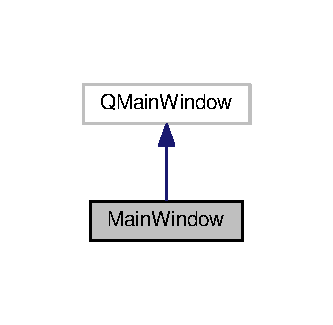
\includegraphics[width=160pt]{classMainWindow__inherit__graph}
\end{center}
\end{figure}


Collaboration diagram for Main\+Window\+:
\nopagebreak
\begin{figure}[H]
\begin{center}
\leavevmode
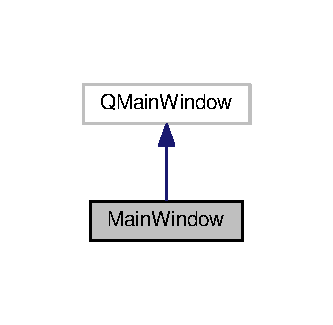
\includegraphics[width=160pt]{classMainWindow__coll__graph}
\end{center}
\end{figure}
\subsection*{Public Slots}
\begin{DoxyCompactItemize}
\item 
void \hyperlink{classMainWindow_a91ab701961139d21df1c4f8d7b31b870}{set\+X\+Rotation} (int angle)
\begin{DoxyCompactList}\small\item\em Slot to set Xrotation angle (either from slider or mouse hold and drag movement). \end{DoxyCompactList}\item 
void \hyperlink{classMainWindow_a023c99cfbdddc154e639d4d53b56a874}{set\+Y\+Rotation} (int angle)
\begin{DoxyCompactList}\small\item\em Slot to set Yrotation angle (either from slider or mouse hold and drag movement). \end{DoxyCompactList}\item 
void \hyperlink{classMainWindow_a3069f073ff2ba99fd601f4f607e77f8b}{set\+Z\+Rotation} (int angle)
\begin{DoxyCompactList}\small\item\em Slot to set Zrotation (either from slider or mouse hold and drag movement). \end{DoxyCompactList}\end{DoxyCompactItemize}
\subsection*{Signals}
\begin{DoxyCompactItemize}
\item 
void \hyperlink{classMainWindow_a752903ab754e432c12f954ea872c854c}{x\+Rotation\+Changed} (int angle)
\begin{DoxyCompactList}\small\item\em Signal to inform slider that x rotation angle has been changed by mouse hold and drag movement. \end{DoxyCompactList}\item 
void \hyperlink{classMainWindow_a4c0058cde1d49828b803919dfbf771c4}{y\+Rotation\+Changed} (int angle)
\begin{DoxyCompactList}\small\item\em Signal to inform slider that y rotation angle has been changed by mouse hold and drag movement. \end{DoxyCompactList}\item 
void \hyperlink{classMainWindow_a08d6c28ab348ab6626abf0168e73cd1d}{z\+Rotation\+Changed} (int angle)
\begin{DoxyCompactList}\small\item\em Signal to inform slider that z rotation angle has been changed by mouse hold and drag movement. \end{DoxyCompactList}\end{DoxyCompactItemize}
\subsection*{Public Member Functions}
\begin{DoxyCompactItemize}
\item 
\hyperlink{classMainWindow_a8b244be8b7b7db1b08de2a2acb9409db}{Main\+Window} (Q\+Widget $\ast$parent=0)
\begin{DoxyCompactList}\small\item\em Required constructor to setup UI. \end{DoxyCompactList}\item 
\hyperlink{classMainWindow_ae98d00a93bc118200eeef9f9bba1dba7}{$\sim$\+Main\+Window} ()
\begin{DoxyCompactList}\small\item\em Required Destructor. \end{DoxyCompactList}\item 
void \hyperlink{classMainWindow_ad61780253f03d8089d2e928a3113baf8}{set\+Vertices} (std\+::vector$<$ \hyperlink{structVertice}{Vertice} $>$ \&out\+\_\+vertices, std\+::vector$<$ std\+::vector$<$ unsigned int $>$ $>$ \&faces\+\_\+vertices)
\begin{DoxyCompactList}\small\item\em Function used to set Vertices of the 3d figure (Used for 3d to 2d views). \end{DoxyCompactList}\item 
void \hyperlink{classMainWindow_a9a9324e1f5908834f69b5a7944fcbc38}{set\+Wire\+Frame} (\hyperlink{classWireFrame}{Wire\+Frame} wf)
\begin{DoxyCompactList}\small\item\em Function used to set the Wireframe object generated from labelled 2d Views. \end{DoxyCompactList}\item 
void \hyperlink{classMainWindow_abfa616ee6054f649786c044555289380}{render2\+Din\+Label} (\hyperlink{classFig3D}{Fig3D} \&fig\+\_\+to\+\_\+render, unsigned int plane)
\begin{DoxyCompactList}\small\item\em Function used to render the view in a specific label according to number set by plane. \end{DoxyCompactList}\item 
void \hyperlink{classMainWindow_a8c1191ba31eb843bede258cd5fdc571e}{render\+All\+Views} (\hyperlink{classFig3D}{Fig3D} \&fig\+\_\+to\+\_\+render)
\begin{DoxyCompactList}\small\item\em Function used to render all views of a 3d figure. \end{DoxyCompactList}\item 
void \hyperlink{classMainWindow_a6ae88293630f79a3ccb75bc5e64daea5}{incX} ()
\begin{DoxyCompactList}\small\item\em Function used to increase X offset of displayed figure. \end{DoxyCompactList}\item 
void \hyperlink{classMainWindow_ad4fa62f605231f2c935f37f7a204bbf9}{incY} ()
\begin{DoxyCompactList}\small\item\em Function used to increase Y offset of displayed figure. \end{DoxyCompactList}\item 
void \hyperlink{classMainWindow_a25ae6019ab87c5e9bf844ac007b00249}{incZ} ()
\begin{DoxyCompactList}\small\item\em Function used to increase Z offset of displayed figure. \end{DoxyCompactList}\item 
void \hyperlink{classMainWindow_a4c4ad4dbc9064c0bdbdb5f9ba619a6c2}{decX} ()
\begin{DoxyCompactList}\small\item\em Function used to decrease X offset of displayed figure. \end{DoxyCompactList}\item 
void \hyperlink{classMainWindow_aeab655f19703fca45999fc3cb11b6bd0}{decY} ()
\begin{DoxyCompactList}\small\item\em Function used to decrease Y offset of displayed figure. \end{DoxyCompactList}\item 
void \hyperlink{classMainWindow_a5841a993bb0167306794580058c435e2}{decZ} ()
\begin{DoxyCompactList}\small\item\em Function used to decrease Z offset of displayed figure. \end{DoxyCompactList}\item 
void \hyperlink{classMainWindow_a571790691bad25c9861c0c487ba0ce43}{zoomin} ()
\begin{DoxyCompactList}\small\item\em Function used to increase scaling or zooming in of displayed figure. \end{DoxyCompactList}\item 
void \hyperlink{classMainWindow_ac54938e78f6b39c6b62cee61d75e8c22}{zoomout} ()
\begin{DoxyCompactList}\small\item\em Function used to decrease scaling or zooming out of displayed figure. \end{DoxyCompactList}\item 
void \hyperlink{classMainWindow_a128f71880d4b9683149023fc46fcc9f8}{update} ()
\begin{DoxyCompactList}\small\item\em Function triggered to reconstruct views whenever offset or rotation of object changed. \end{DoxyCompactList}\item 
void \hyperlink{classMainWindow_a1dff511c9697cbcb60150894f480b9c8}{mouse\+Press\+Event} (Q\+Mouse\+Event $\ast$event) override
\begin{DoxyCompactList}\small\item\em Function to handle mouse press events. \end{DoxyCompactList}\item 
void \hyperlink{classMainWindow_a9c8748d463f01ddae6abcd8f8163fcef}{mouse\+Move\+Event} (Q\+Mouse\+Event $\ast$event) override
\begin{DoxyCompactList}\small\item\em Function to handle movement of mouse after clicking. \end{DoxyCompactList}\item 
void \hyperlink{classMainWindow_a3309de2dae8bbfaf0ff645fe372aa644}{render\+From\+Edges} (vector$<$ \hyperlink{structEdge}{Edge} $>$ edges, int plane)
\begin{DoxyCompactList}\small\item\em Function used to render views from the given edges. \end{DoxyCompactList}\item 
void \hyperlink{classMainWindow_a91288f71f3b29443c1243ddb653f3898}{render2\+Dto3D} (\hyperlink{classWireFrame}{Wire\+Frame} wf, \hyperlink{classFig3D}{Fig3D} fig)
\begin{DoxyCompactList}\small\item\em Function used to render the views from the provided wireframe (in case of 2d to 3d) \end{DoxyCompactList}\item 
void \hyperlink{classMainWindow_acc4ea38c583bc825f258ab2ec432e835}{connect\+Sliderand\+Buttons} ()
\begin{DoxyCompactList}\small\item\em Function to connect all sliders and buttons to appropriate functions on initializing view. \end{DoxyCompactList}\end{DoxyCompactItemize}
\subsection*{Public Attributes}
\begin{DoxyCompactItemize}
\item 
int \hyperlink{classMainWindow_a0d680234c97ecdc151020dd0ec09cc54}{mode}
\end{DoxyCompactItemize}


\subsection{Constructor \& Destructor Documentation}
\mbox{\Hypertarget{classMainWindow_a8b244be8b7b7db1b08de2a2acb9409db}\label{classMainWindow_a8b244be8b7b7db1b08de2a2acb9409db}} 
\index{Main\+Window@{Main\+Window}!Main\+Window@{Main\+Window}}
\index{Main\+Window@{Main\+Window}!Main\+Window@{Main\+Window}}
\subsubsection{\texorpdfstring{Main\+Window()}{MainWindow()}}
{\footnotesize\ttfamily Main\+Window\+::\+Main\+Window (\begin{DoxyParamCaption}\item[{Q\+Widget $\ast$}]{parent = {\ttfamily 0} }\end{DoxyParamCaption})\hspace{0.3cm}{\ttfamily [explicit]}}



Required constructor to setup UI. 

\mbox{\Hypertarget{classMainWindow_ae98d00a93bc118200eeef9f9bba1dba7}\label{classMainWindow_ae98d00a93bc118200eeef9f9bba1dba7}} 
\index{Main\+Window@{Main\+Window}!````~Main\+Window@{$\sim$\+Main\+Window}}
\index{````~Main\+Window@{$\sim$\+Main\+Window}!Main\+Window@{Main\+Window}}
\subsubsection{\texorpdfstring{$\sim$\+Main\+Window()}{~MainWindow()}}
{\footnotesize\ttfamily Main\+Window\+::$\sim$\+Main\+Window (\begin{DoxyParamCaption}{ }\end{DoxyParamCaption})}



Required Destructor. 



\subsection{Member Function Documentation}
\mbox{\Hypertarget{classMainWindow_acc4ea38c583bc825f258ab2ec432e835}\label{classMainWindow_acc4ea38c583bc825f258ab2ec432e835}} 
\index{Main\+Window@{Main\+Window}!connect\+Sliderand\+Buttons@{connect\+Sliderand\+Buttons}}
\index{connect\+Sliderand\+Buttons@{connect\+Sliderand\+Buttons}!Main\+Window@{Main\+Window}}
\subsubsection{\texorpdfstring{connect\+Sliderand\+Buttons()}{connectSliderandButtons()}}
{\footnotesize\ttfamily void Main\+Window\+::connect\+Sliderand\+Buttons (\begin{DoxyParamCaption}{ }\end{DoxyParamCaption})}



Function to connect all sliders and buttons to appropriate functions on initializing view. 

\mbox{\Hypertarget{classMainWindow_a4c4ad4dbc9064c0bdbdb5f9ba619a6c2}\label{classMainWindow_a4c4ad4dbc9064c0bdbdb5f9ba619a6c2}} 
\index{Main\+Window@{Main\+Window}!decX@{decX}}
\index{decX@{decX}!Main\+Window@{Main\+Window}}
\subsubsection{\texorpdfstring{dec\+X()}{decX()}}
{\footnotesize\ttfamily void Main\+Window\+::decX (\begin{DoxyParamCaption}{ }\end{DoxyParamCaption})}



Function used to decrease X offset of displayed figure. 

\mbox{\Hypertarget{classMainWindow_aeab655f19703fca45999fc3cb11b6bd0}\label{classMainWindow_aeab655f19703fca45999fc3cb11b6bd0}} 
\index{Main\+Window@{Main\+Window}!decY@{decY}}
\index{decY@{decY}!Main\+Window@{Main\+Window}}
\subsubsection{\texorpdfstring{dec\+Y()}{decY()}}
{\footnotesize\ttfamily void Main\+Window\+::decY (\begin{DoxyParamCaption}{ }\end{DoxyParamCaption})}



Function used to decrease Y offset of displayed figure. 

\mbox{\Hypertarget{classMainWindow_a5841a993bb0167306794580058c435e2}\label{classMainWindow_a5841a993bb0167306794580058c435e2}} 
\index{Main\+Window@{Main\+Window}!decZ@{decZ}}
\index{decZ@{decZ}!Main\+Window@{Main\+Window}}
\subsubsection{\texorpdfstring{dec\+Z()}{decZ()}}
{\footnotesize\ttfamily void Main\+Window\+::decZ (\begin{DoxyParamCaption}{ }\end{DoxyParamCaption})}



Function used to decrease Z offset of displayed figure. 

\mbox{\Hypertarget{classMainWindow_a6ae88293630f79a3ccb75bc5e64daea5}\label{classMainWindow_a6ae88293630f79a3ccb75bc5e64daea5}} 
\index{Main\+Window@{Main\+Window}!incX@{incX}}
\index{incX@{incX}!Main\+Window@{Main\+Window}}
\subsubsection{\texorpdfstring{inc\+X()}{incX()}}
{\footnotesize\ttfamily void Main\+Window\+::incX (\begin{DoxyParamCaption}{ }\end{DoxyParamCaption})}



Function used to increase X offset of displayed figure. 

\mbox{\Hypertarget{classMainWindow_ad4fa62f605231f2c935f37f7a204bbf9}\label{classMainWindow_ad4fa62f605231f2c935f37f7a204bbf9}} 
\index{Main\+Window@{Main\+Window}!incY@{incY}}
\index{incY@{incY}!Main\+Window@{Main\+Window}}
\subsubsection{\texorpdfstring{inc\+Y()}{incY()}}
{\footnotesize\ttfamily void Main\+Window\+::incY (\begin{DoxyParamCaption}{ }\end{DoxyParamCaption})}



Function used to increase Y offset of displayed figure. 

\mbox{\Hypertarget{classMainWindow_a25ae6019ab87c5e9bf844ac007b00249}\label{classMainWindow_a25ae6019ab87c5e9bf844ac007b00249}} 
\index{Main\+Window@{Main\+Window}!incZ@{incZ}}
\index{incZ@{incZ}!Main\+Window@{Main\+Window}}
\subsubsection{\texorpdfstring{inc\+Z()}{incZ()}}
{\footnotesize\ttfamily void Main\+Window\+::incZ (\begin{DoxyParamCaption}{ }\end{DoxyParamCaption})}



Function used to increase Z offset of displayed figure. 

\mbox{\Hypertarget{classMainWindow_a9c8748d463f01ddae6abcd8f8163fcef}\label{classMainWindow_a9c8748d463f01ddae6abcd8f8163fcef}} 
\index{Main\+Window@{Main\+Window}!mouse\+Move\+Event@{mouse\+Move\+Event}}
\index{mouse\+Move\+Event@{mouse\+Move\+Event}!Main\+Window@{Main\+Window}}
\subsubsection{\texorpdfstring{mouse\+Move\+Event()}{mouseMoveEvent()}}
{\footnotesize\ttfamily void Main\+Window\+::mouse\+Move\+Event (\begin{DoxyParamCaption}\item[{Q\+Mouse\+Event $\ast$}]{event }\end{DoxyParamCaption})\hspace{0.3cm}{\ttfamily [override]}}



Function to handle movement of mouse after clicking. 

\mbox{\Hypertarget{classMainWindow_a1dff511c9697cbcb60150894f480b9c8}\label{classMainWindow_a1dff511c9697cbcb60150894f480b9c8}} 
\index{Main\+Window@{Main\+Window}!mouse\+Press\+Event@{mouse\+Press\+Event}}
\index{mouse\+Press\+Event@{mouse\+Press\+Event}!Main\+Window@{Main\+Window}}
\subsubsection{\texorpdfstring{mouse\+Press\+Event()}{mousePressEvent()}}
{\footnotesize\ttfamily void Main\+Window\+::mouse\+Press\+Event (\begin{DoxyParamCaption}\item[{Q\+Mouse\+Event $\ast$}]{event }\end{DoxyParamCaption})\hspace{0.3cm}{\ttfamily [override]}}



Function to handle mouse press events. 

\mbox{\Hypertarget{classMainWindow_abfa616ee6054f649786c044555289380}\label{classMainWindow_abfa616ee6054f649786c044555289380}} 
\index{Main\+Window@{Main\+Window}!render2\+Din\+Label@{render2\+Din\+Label}}
\index{render2\+Din\+Label@{render2\+Din\+Label}!Main\+Window@{Main\+Window}}
\subsubsection{\texorpdfstring{render2\+Din\+Label()}{render2DinLabel()}}
{\footnotesize\ttfamily void Main\+Window\+::render2\+Din\+Label (\begin{DoxyParamCaption}\item[{\hyperlink{classFig3D}{Fig3D} \&}]{fig\+\_\+to\+\_\+render,  }\item[{unsigned int}]{plane }\end{DoxyParamCaption})}



Function used to render the view in a specific label according to number set by plane. 

Takes input 3D object information (vertices,faces), Q\+Painter object, othographic plane (XY /\+Y\+Z/ XZ) and draws the corresponding 2D view on the Q\+Painter object \mbox{\Hypertarget{classMainWindow_a91288f71f3b29443c1243ddb653f3898}\label{classMainWindow_a91288f71f3b29443c1243ddb653f3898}} 
\index{Main\+Window@{Main\+Window}!render2\+Dto3D@{render2\+Dto3D}}
\index{render2\+Dto3D@{render2\+Dto3D}!Main\+Window@{Main\+Window}}
\subsubsection{\texorpdfstring{render2\+Dto3\+D()}{render2Dto3D()}}
{\footnotesize\ttfamily void Main\+Window\+::render2\+Dto3D (\begin{DoxyParamCaption}\item[{\hyperlink{classWireFrame}{Wire\+Frame}}]{wf,  }\item[{\hyperlink{classFig3D}{Fig3D}}]{fig }\end{DoxyParamCaption})}



Function used to render the views from the provided wireframe (in case of 2d to 3d) 

\mbox{\Hypertarget{classMainWindow_a8c1191ba31eb843bede258cd5fdc571e}\label{classMainWindow_a8c1191ba31eb843bede258cd5fdc571e}} 
\index{Main\+Window@{Main\+Window}!render\+All\+Views@{render\+All\+Views}}
\index{render\+All\+Views@{render\+All\+Views}!Main\+Window@{Main\+Window}}
\subsubsection{\texorpdfstring{render\+All\+Views()}{renderAllViews()}}
{\footnotesize\ttfamily void Main\+Window\+::render\+All\+Views (\begin{DoxyParamCaption}\item[{\hyperlink{classFig3D}{Fig3D} \&}]{fig\+\_\+to\+\_\+render }\end{DoxyParamCaption})}



Function used to render all views of a 3d figure. 

\mbox{\Hypertarget{classMainWindow_a3309de2dae8bbfaf0ff645fe372aa644}\label{classMainWindow_a3309de2dae8bbfaf0ff645fe372aa644}} 
\index{Main\+Window@{Main\+Window}!render\+From\+Edges@{render\+From\+Edges}}
\index{render\+From\+Edges@{render\+From\+Edges}!Main\+Window@{Main\+Window}}
\subsubsection{\texorpdfstring{render\+From\+Edges()}{renderFromEdges()}}
{\footnotesize\ttfamily void Main\+Window\+::render\+From\+Edges (\begin{DoxyParamCaption}\item[{vector$<$ \hyperlink{structEdge}{Edge} $>$}]{edges,  }\item[{int}]{plane }\end{DoxyParamCaption})}



Function used to render views from the given edges. 

\mbox{\Hypertarget{classMainWindow_ad61780253f03d8089d2e928a3113baf8}\label{classMainWindow_ad61780253f03d8089d2e928a3113baf8}} 
\index{Main\+Window@{Main\+Window}!set\+Vertices@{set\+Vertices}}
\index{set\+Vertices@{set\+Vertices}!Main\+Window@{Main\+Window}}
\subsubsection{\texorpdfstring{set\+Vertices()}{setVertices()}}
{\footnotesize\ttfamily void Main\+Window\+::set\+Vertices (\begin{DoxyParamCaption}\item[{std\+::vector$<$ \hyperlink{structVertice}{Vertice} $>$ \&}]{out\+\_\+vertices,  }\item[{std\+::vector$<$ std\+::vector$<$ unsigned int $>$ $>$ \&}]{faces\+\_\+vertices }\end{DoxyParamCaption})}



Function used to set Vertices of the 3d figure (Used for 3d to 2d views). 

\mbox{\Hypertarget{classMainWindow_a9a9324e1f5908834f69b5a7944fcbc38}\label{classMainWindow_a9a9324e1f5908834f69b5a7944fcbc38}} 
\index{Main\+Window@{Main\+Window}!set\+Wire\+Frame@{set\+Wire\+Frame}}
\index{set\+Wire\+Frame@{set\+Wire\+Frame}!Main\+Window@{Main\+Window}}
\subsubsection{\texorpdfstring{set\+Wire\+Frame()}{setWireFrame()}}
{\footnotesize\ttfamily void Main\+Window\+::set\+Wire\+Frame (\begin{DoxyParamCaption}\item[{\hyperlink{classWireFrame}{Wire\+Frame}}]{wf }\end{DoxyParamCaption})}



Function used to set the Wireframe object generated from labelled 2d Views. 

\mbox{\Hypertarget{classMainWindow_a91ab701961139d21df1c4f8d7b31b870}\label{classMainWindow_a91ab701961139d21df1c4f8d7b31b870}} 
\index{Main\+Window@{Main\+Window}!set\+X\+Rotation@{set\+X\+Rotation}}
\index{set\+X\+Rotation@{set\+X\+Rotation}!Main\+Window@{Main\+Window}}
\subsubsection{\texorpdfstring{set\+X\+Rotation}{setXRotation}}
{\footnotesize\ttfamily void Main\+Window\+::set\+X\+Rotation (\begin{DoxyParamCaption}\item[{int}]{angle }\end{DoxyParamCaption})\hspace{0.3cm}{\ttfamily [slot]}}



Slot to set Xrotation angle (either from slider or mouse hold and drag movement). 

\mbox{\Hypertarget{classMainWindow_a023c99cfbdddc154e639d4d53b56a874}\label{classMainWindow_a023c99cfbdddc154e639d4d53b56a874}} 
\index{Main\+Window@{Main\+Window}!set\+Y\+Rotation@{set\+Y\+Rotation}}
\index{set\+Y\+Rotation@{set\+Y\+Rotation}!Main\+Window@{Main\+Window}}
\subsubsection{\texorpdfstring{set\+Y\+Rotation}{setYRotation}}
{\footnotesize\ttfamily void Main\+Window\+::set\+Y\+Rotation (\begin{DoxyParamCaption}\item[{int}]{angle }\end{DoxyParamCaption})\hspace{0.3cm}{\ttfamily [slot]}}



Slot to set Yrotation angle (either from slider or mouse hold and drag movement). 

\mbox{\Hypertarget{classMainWindow_a3069f073ff2ba99fd601f4f607e77f8b}\label{classMainWindow_a3069f073ff2ba99fd601f4f607e77f8b}} 
\index{Main\+Window@{Main\+Window}!set\+Z\+Rotation@{set\+Z\+Rotation}}
\index{set\+Z\+Rotation@{set\+Z\+Rotation}!Main\+Window@{Main\+Window}}
\subsubsection{\texorpdfstring{set\+Z\+Rotation}{setZRotation}}
{\footnotesize\ttfamily void Main\+Window\+::set\+Z\+Rotation (\begin{DoxyParamCaption}\item[{int}]{angle }\end{DoxyParamCaption})\hspace{0.3cm}{\ttfamily [slot]}}



Slot to set Zrotation (either from slider or mouse hold and drag movement). 

\mbox{\Hypertarget{classMainWindow_a128f71880d4b9683149023fc46fcc9f8}\label{classMainWindow_a128f71880d4b9683149023fc46fcc9f8}} 
\index{Main\+Window@{Main\+Window}!update@{update}}
\index{update@{update}!Main\+Window@{Main\+Window}}
\subsubsection{\texorpdfstring{update()}{update()}}
{\footnotesize\ttfamily void Main\+Window\+::update (\begin{DoxyParamCaption}{ }\end{DoxyParamCaption})}



Function triggered to reconstruct views whenever offset or rotation of object changed. 

\mbox{\Hypertarget{classMainWindow_a752903ab754e432c12f954ea872c854c}\label{classMainWindow_a752903ab754e432c12f954ea872c854c}} 
\index{Main\+Window@{Main\+Window}!x\+Rotation\+Changed@{x\+Rotation\+Changed}}
\index{x\+Rotation\+Changed@{x\+Rotation\+Changed}!Main\+Window@{Main\+Window}}
\subsubsection{\texorpdfstring{x\+Rotation\+Changed}{xRotationChanged}}
{\footnotesize\ttfamily void Main\+Window\+::x\+Rotation\+Changed (\begin{DoxyParamCaption}\item[{int}]{angle }\end{DoxyParamCaption})\hspace{0.3cm}{\ttfamily [signal]}}



Signal to inform slider that x rotation angle has been changed by mouse hold and drag movement. 

\mbox{\Hypertarget{classMainWindow_a4c0058cde1d49828b803919dfbf771c4}\label{classMainWindow_a4c0058cde1d49828b803919dfbf771c4}} 
\index{Main\+Window@{Main\+Window}!y\+Rotation\+Changed@{y\+Rotation\+Changed}}
\index{y\+Rotation\+Changed@{y\+Rotation\+Changed}!Main\+Window@{Main\+Window}}
\subsubsection{\texorpdfstring{y\+Rotation\+Changed}{yRotationChanged}}
{\footnotesize\ttfamily void Main\+Window\+::y\+Rotation\+Changed (\begin{DoxyParamCaption}\item[{int}]{angle }\end{DoxyParamCaption})\hspace{0.3cm}{\ttfamily [signal]}}



Signal to inform slider that y rotation angle has been changed by mouse hold and drag movement. 

\mbox{\Hypertarget{classMainWindow_a571790691bad25c9861c0c487ba0ce43}\label{classMainWindow_a571790691bad25c9861c0c487ba0ce43}} 
\index{Main\+Window@{Main\+Window}!zoomin@{zoomin}}
\index{zoomin@{zoomin}!Main\+Window@{Main\+Window}}
\subsubsection{\texorpdfstring{zoomin()}{zoomin()}}
{\footnotesize\ttfamily void Main\+Window\+::zoomin (\begin{DoxyParamCaption}{ }\end{DoxyParamCaption})}



Function used to increase scaling or zooming in of displayed figure. 

\mbox{\Hypertarget{classMainWindow_ac54938e78f6b39c6b62cee61d75e8c22}\label{classMainWindow_ac54938e78f6b39c6b62cee61d75e8c22}} 
\index{Main\+Window@{Main\+Window}!zoomout@{zoomout}}
\index{zoomout@{zoomout}!Main\+Window@{Main\+Window}}
\subsubsection{\texorpdfstring{zoomout()}{zoomout()}}
{\footnotesize\ttfamily void Main\+Window\+::zoomout (\begin{DoxyParamCaption}{ }\end{DoxyParamCaption})}



Function used to decrease scaling or zooming out of displayed figure. 

\mbox{\Hypertarget{classMainWindow_a08d6c28ab348ab6626abf0168e73cd1d}\label{classMainWindow_a08d6c28ab348ab6626abf0168e73cd1d}} 
\index{Main\+Window@{Main\+Window}!z\+Rotation\+Changed@{z\+Rotation\+Changed}}
\index{z\+Rotation\+Changed@{z\+Rotation\+Changed}!Main\+Window@{Main\+Window}}
\subsubsection{\texorpdfstring{z\+Rotation\+Changed}{zRotationChanged}}
{\footnotesize\ttfamily void Main\+Window\+::z\+Rotation\+Changed (\begin{DoxyParamCaption}\item[{int}]{angle }\end{DoxyParamCaption})\hspace{0.3cm}{\ttfamily [signal]}}



Signal to inform slider that z rotation angle has been changed by mouse hold and drag movement. 



\subsection{Member Data Documentation}
\mbox{\Hypertarget{classMainWindow_a0d680234c97ecdc151020dd0ec09cc54}\label{classMainWindow_a0d680234c97ecdc151020dd0ec09cc54}} 
\index{Main\+Window@{Main\+Window}!mode@{mode}}
\index{mode@{mode}!Main\+Window@{Main\+Window}}
\subsubsection{\texorpdfstring{mode}{mode}}
{\footnotesize\ttfamily int Main\+Window\+::mode}



The documentation for this class was generated from the following files\+:\begin{DoxyCompactItemize}
\item 
/home/ankurshaswat/\+My\+Files/\+Repos/\+C\+O\+P290-\/master/\+E\+D\+\_\+\+Project/include/\hyperlink{mainwindow_8h}{mainwindow.\+h}\item 
/home/ankurshaswat/\+My\+Files/\+Repos/\+C\+O\+P290-\/master/\+E\+D\+\_\+\+Project/src/\hyperlink{mainwindow_8cpp}{mainwindow.\+cpp}\end{DoxyCompactItemize}

\hypertarget{classoptionWindow}{}\section{option\+Window Class Reference}
\label{classoptionWindow}\index{option\+Window@{option\+Window}}


{\ttfamily \#include $<$optionwindow.\+h$>$}



Inheritance diagram for option\+Window\+:
\nopagebreak
\begin{figure}[H]
\begin{center}
\leavevmode
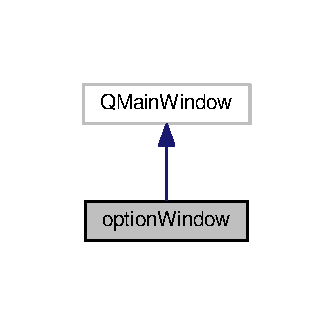
\includegraphics[width=160pt]{classoptionWindow__inherit__graph}
\end{center}
\end{figure}


Collaboration diagram for option\+Window\+:
\nopagebreak
\begin{figure}[H]
\begin{center}
\leavevmode
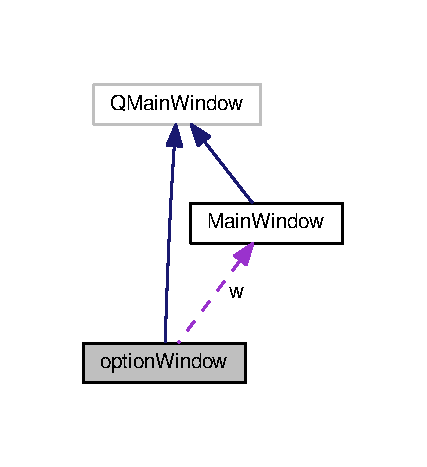
\includegraphics[width=205pt]{classoptionWindow__coll__graph}
\end{center}
\end{figure}
\subsection*{Public Member Functions}
\begin{DoxyCompactItemize}
\item 
\hyperlink{classoptionWindow_a520eacaa5cabadee57621a9a24345302}{option\+Window} (Q\+Widget $\ast$parent=0)
\item 
\hyperlink{classoptionWindow_a767beb27d15754996076ff312ae2877f}{$\sim$option\+Window} ()
\end{DoxyCompactItemize}
\subsection*{Public Attributes}
\begin{DoxyCompactItemize}
\item 
\hyperlink{classMainWindow}{Main\+Window} \hyperlink{classoptionWindow_a3f43dd31b7b6836835ae91bff4f22e2a}{w}
\end{DoxyCompactItemize}


\subsection{Constructor \& Destructor Documentation}
\mbox{\Hypertarget{classoptionWindow_a520eacaa5cabadee57621a9a24345302}\label{classoptionWindow_a520eacaa5cabadee57621a9a24345302}} 
\index{option\+Window@{option\+Window}!option\+Window@{option\+Window}}
\index{option\+Window@{option\+Window}!option\+Window@{option\+Window}}
\subsubsection{\texorpdfstring{option\+Window()}{optionWindow()}}
{\footnotesize\ttfamily option\+Window\+::option\+Window (\begin{DoxyParamCaption}\item[{Q\+Widget $\ast$}]{parent = {\ttfamily 0} }\end{DoxyParamCaption})\hspace{0.3cm}{\ttfamily [explicit]}}

\mbox{\Hypertarget{classoptionWindow_a767beb27d15754996076ff312ae2877f}\label{classoptionWindow_a767beb27d15754996076ff312ae2877f}} 
\index{option\+Window@{option\+Window}!````~option\+Window@{$\sim$option\+Window}}
\index{````~option\+Window@{$\sim$option\+Window}!option\+Window@{option\+Window}}
\subsubsection{\texorpdfstring{$\sim$option\+Window()}{~optionWindow()}}
{\footnotesize\ttfamily option\+Window\+::$\sim$option\+Window (\begin{DoxyParamCaption}{ }\end{DoxyParamCaption})}



\subsection{Member Data Documentation}
\mbox{\Hypertarget{classoptionWindow_a3f43dd31b7b6836835ae91bff4f22e2a}\label{classoptionWindow_a3f43dd31b7b6836835ae91bff4f22e2a}} 
\index{option\+Window@{option\+Window}!w@{w}}
\index{w@{w}!option\+Window@{option\+Window}}
\subsubsection{\texorpdfstring{w}{w}}
{\footnotesize\ttfamily \hyperlink{classMainWindow}{Main\+Window} option\+Window\+::w}



The documentation for this class was generated from the following files\+:\begin{DoxyCompactItemize}
\item 
/home/ankurshaswat/\+My\+Files/\+Repos/\+C\+O\+P290/working\+\_\+3d\+\_\+to\+\_\+2d/\hyperlink{optionwindow_8h}{optionwindow.\+h}\item 
/home/ankurshaswat/\+My\+Files/\+Repos/\+C\+O\+P290/working\+\_\+3d\+\_\+to\+\_\+2d/\hyperlink{optionwindow_8cpp}{optionwindow.\+cpp}\end{DoxyCompactItemize}

\hypertarget{classpartialOrder}{}\section{partial\+Order Class Reference}
\label{classpartialOrder}\index{partial\+Order@{partial\+Order}}


{\ttfamily \#include $<$structs.\+h$>$}



\subsection{Detailed Description}
Custom data structures needed in reconstruction 

The documentation for this class was generated from the following file\+:\begin{DoxyCompactItemize}
\item 
/home/ankurshaswat/\+My\+Files/\+Repos/\+C\+O\+P290/\+Project1/\+Code/include/module1/\hyperlink{structs_8h}{structs.\+h}\end{DoxyCompactItemize}

\hypertarget{structPlane}{}\section{Plane Struct Reference}
\label{structPlane}\index{Plane@{Plane}}


Structured Defined to represent Planes.  




{\ttfamily \#include $<$basic\+Components.\+h$>$}

\subsection*{Public Member Functions}
\begin{DoxyCompactItemize}
\item 
\hyperlink{structPlane_a96a24212b7af50908a3c62f40b9c26c9}{Plane} (\hyperlink{structVertice}{Vertice} u, \hyperlink{structVertice}{Vertice} v, \hyperlink{structVertice}{Vertice} w)
\begin{DoxyCompactList}\small\item\em Constructor to define plane using 3 vertices. \end{DoxyCompactList}\item 
float \hyperlink{structPlane_a05bbcf26965e39ed9e95a8cb41269f5c}{distance} (\hyperlink{structVertice}{Vertice} u)
\item 
bool \hyperlink{structPlane_a3a525d011cf5214cf9223976ce113876}{on\+Plane} (\hyperlink{structEdge}{Edge} e)
\begin{DoxyCompactList}\small\item\em Function used to check whether an \hyperlink{structEdge}{Edge} lies on the plane or not. \end{DoxyCompactList}\end{DoxyCompactItemize}
\subsection*{Public Attributes}
\begin{DoxyCompactItemize}
\item 
float \hyperlink{structPlane_a818b693ba813d53949e18aa1416cc12a}{a}
\item 
float \hyperlink{structPlane_a3d802fea10cfe6352e1792733d793b14}{b}
\item 
float \hyperlink{structPlane_aec04c57607ffa16c210f955360ef4153}{c}
\item 
float \hyperlink{structPlane_a61fc789fce8fbe72914f5397f1bbed44}{d}
\end{DoxyCompactItemize}


\subsection{Detailed Description}
Structured Defined to represent Planes. 

\subsection{Constructor \& Destructor Documentation}
\mbox{\Hypertarget{structPlane_a96a24212b7af50908a3c62f40b9c26c9}\label{structPlane_a96a24212b7af50908a3c62f40b9c26c9}} 
\index{Plane@{Plane}!Plane@{Plane}}
\index{Plane@{Plane}!Plane@{Plane}}
\subsubsection{\texorpdfstring{Plane()}{Plane()}}
{\footnotesize\ttfamily Plane\+::\+Plane (\begin{DoxyParamCaption}\item[{\hyperlink{structVertice}{Vertice}}]{u,  }\item[{\hyperlink{structVertice}{Vertice}}]{v,  }\item[{\hyperlink{structVertice}{Vertice}}]{w }\end{DoxyParamCaption})\hspace{0.3cm}{\ttfamily [inline]}}



Constructor to define plane using 3 vertices. 



\subsection{Member Function Documentation}
\mbox{\Hypertarget{structPlane_a05bbcf26965e39ed9e95a8cb41269f5c}\label{structPlane_a05bbcf26965e39ed9e95a8cb41269f5c}} 
\index{Plane@{Plane}!distance@{distance}}
\index{distance@{distance}!Plane@{Plane}}
\subsubsection{\texorpdfstring{distance()}{distance()}}
{\footnotesize\ttfamily float Plane\+::distance (\begin{DoxyParamCaption}\item[{\hyperlink{structVertice}{Vertice}}]{u }\end{DoxyParamCaption})\hspace{0.3cm}{\ttfamily [inline]}}

\mbox{\Hypertarget{structPlane_a3a525d011cf5214cf9223976ce113876}\label{structPlane_a3a525d011cf5214cf9223976ce113876}} 
\index{Plane@{Plane}!on\+Plane@{on\+Plane}}
\index{on\+Plane@{on\+Plane}!Plane@{Plane}}
\subsubsection{\texorpdfstring{on\+Plane()}{onPlane()}}
{\footnotesize\ttfamily bool Plane\+::on\+Plane (\begin{DoxyParamCaption}\item[{\hyperlink{structEdge}{Edge}}]{e }\end{DoxyParamCaption})\hspace{0.3cm}{\ttfamily [inline]}}



Function used to check whether an \hyperlink{structEdge}{Edge} lies on the plane or not. 



\subsection{Member Data Documentation}
\mbox{\Hypertarget{structPlane_a818b693ba813d53949e18aa1416cc12a}\label{structPlane_a818b693ba813d53949e18aa1416cc12a}} 
\index{Plane@{Plane}!a@{a}}
\index{a@{a}!Plane@{Plane}}
\subsubsection{\texorpdfstring{a}{a}}
{\footnotesize\ttfamily float Plane\+::a}

\mbox{\Hypertarget{structPlane_a3d802fea10cfe6352e1792733d793b14}\label{structPlane_a3d802fea10cfe6352e1792733d793b14}} 
\index{Plane@{Plane}!b@{b}}
\index{b@{b}!Plane@{Plane}}
\subsubsection{\texorpdfstring{b}{b}}
{\footnotesize\ttfamily float Plane\+::b}

\mbox{\Hypertarget{structPlane_aec04c57607ffa16c210f955360ef4153}\label{structPlane_aec04c57607ffa16c210f955360ef4153}} 
\index{Plane@{Plane}!c@{c}}
\index{c@{c}!Plane@{Plane}}
\subsubsection{\texorpdfstring{c}{c}}
{\footnotesize\ttfamily float Plane\+::c}

\mbox{\Hypertarget{structPlane_a61fc789fce8fbe72914f5397f1bbed44}\label{structPlane_a61fc789fce8fbe72914f5397f1bbed44}} 
\index{Plane@{Plane}!d@{d}}
\index{d@{d}!Plane@{Plane}}
\subsubsection{\texorpdfstring{d}{d}}
{\footnotesize\ttfamily float Plane\+::d}



The documentation for this struct was generated from the following file\+:\begin{DoxyCompactItemize}
\item 
/home/ankurshaswat/\+My\+Files/\+Repos/\+C\+O\+P290-\/master/\+E\+D\+\_\+\+Project/include/\hyperlink{basicComponents_8h}{basic\+Components.\+h}\end{DoxyCompactItemize}

\hypertarget{structVertice}{}\section{Vertice Struct Reference}
\label{structVertice}\index{Vertice@{Vertice}}


{\ttfamily \#include $<$basic\+Components.\+h$>$}

\subsection*{Public Member Functions}
\begin{DoxyCompactItemize}
\item 
\hyperlink{structVertice}{Vertice} \hyperlink{structVertice_a914a6647d86f9f439c1b8751674973ec}{deep\+Copy} ()
\item 
bool \hyperlink{structVertice_a8ed5964130f1d72b0a9ab0ce72506e1d}{operator$<$} (\hyperlink{structVertice}{Vertice} other) const
\begin{DoxyCompactList}\small\item\em Less than operator defined for faster comparisons between different vertices. \end{DoxyCompactList}\item 
bool \hyperlink{structVertice_a17d6154f69e230b4c927fe70e8442f4c}{operator==} (\hyperlink{structVertice}{Vertice} b)
\begin{DoxyCompactList}\small\item\em Equality operator defined for faster comparisons between different vertices. \end{DoxyCompactList}\item 
\hyperlink{structVertice}{Vertice} \hyperlink{structVertice_a2f9bd3f865f0613f41bbc2dd3ac2d08d}{operator-\/} (const \hyperlink{structVertice}{Vertice} \&rhs)
\begin{DoxyCompactList}\small\item\em Difference operator defined for faster comparisons between different vertices. \end{DoxyCompactList}\end{DoxyCompactItemize}
\subsection*{Public Attributes}
\begin{DoxyCompactItemize}
\item 
float \hyperlink{structVertice_a458c4138041414f66cc8234dcb8a76a8}{first}
\item 
float \hyperlink{structVertice_a3b09ccd0c9d23978cb17ebe303b498a2}{second}
\item 
float \hyperlink{structVertice_a781306a1aba368740f76928fc4b3b6bc}{third} =0
\item 
bool \hyperlink{structVertice_ae1b4f2a0c6783f5cf06b6dbcc49f8231}{is3d} =true
\item 
char \hyperlink{structVertice_a0181015506ba076b22502bba2c02f4cf}{label}
\end{DoxyCompactItemize}


\subsection{Member Function Documentation}
\mbox{\Hypertarget{structVertice_a914a6647d86f9f439c1b8751674973ec}\label{structVertice_a914a6647d86f9f439c1b8751674973ec}} 
\index{Vertice@{Vertice}!deep\+Copy@{deep\+Copy}}
\index{deep\+Copy@{deep\+Copy}!Vertice@{Vertice}}
\subsubsection{\texorpdfstring{deep\+Copy()}{deepCopy()}}
{\footnotesize\ttfamily \hyperlink{structVertice}{Vertice} Vertice\+::deep\+Copy (\begin{DoxyParamCaption}{ }\end{DoxyParamCaption})\hspace{0.3cm}{\ttfamily [inline]}}

\begin{DoxyReturn}{Returns}
\hyperlink{structVertice}{Vertice} that is the generated copy
\end{DoxyReturn}
This method generates a copy of the \hyperlink{structVertice}{Vertice} object from which it is called to create a new \hyperlink{structVertice}{Vertice} object with the same values but free from any reference to original. \mbox{\Hypertarget{structVertice_a2f9bd3f865f0613f41bbc2dd3ac2d08d}\label{structVertice_a2f9bd3f865f0613f41bbc2dd3ac2d08d}} 
\index{Vertice@{Vertice}!operator-\/@{operator-\/}}
\index{operator-\/@{operator-\/}!Vertice@{Vertice}}
\subsubsection{\texorpdfstring{operator-\/()}{operator-()}}
{\footnotesize\ttfamily \hyperlink{structVertice}{Vertice} Vertice\+::operator-\/ (\begin{DoxyParamCaption}\item[{const \hyperlink{structVertice}{Vertice} \&}]{rhs }\end{DoxyParamCaption})\hspace{0.3cm}{\ttfamily [inline]}}



Difference operator defined for faster comparisons between different vertices. 

\mbox{\Hypertarget{structVertice_a8ed5964130f1d72b0a9ab0ce72506e1d}\label{structVertice_a8ed5964130f1d72b0a9ab0ce72506e1d}} 
\index{Vertice@{Vertice}!operator$<$@{operator$<$}}
\index{operator$<$@{operator$<$}!Vertice@{Vertice}}
\subsubsection{\texorpdfstring{operator$<$()}{operator<()}}
{\footnotesize\ttfamily bool Vertice\+::operator$<$ (\begin{DoxyParamCaption}\item[{\hyperlink{structVertice}{Vertice}}]{other }\end{DoxyParamCaption}) const\hspace{0.3cm}{\ttfamily [inline]}}



Less than operator defined for faster comparisons between different vertices. 

\mbox{\Hypertarget{structVertice_a17d6154f69e230b4c927fe70e8442f4c}\label{structVertice_a17d6154f69e230b4c927fe70e8442f4c}} 
\index{Vertice@{Vertice}!operator==@{operator==}}
\index{operator==@{operator==}!Vertice@{Vertice}}
\subsubsection{\texorpdfstring{operator==()}{operator==()}}
{\footnotesize\ttfamily bool Vertice\+::operator== (\begin{DoxyParamCaption}\item[{\hyperlink{structVertice}{Vertice}}]{b }\end{DoxyParamCaption})\hspace{0.3cm}{\ttfamily [inline]}}



Equality operator defined for faster comparisons between different vertices. 



\subsection{Member Data Documentation}
\mbox{\Hypertarget{structVertice_a458c4138041414f66cc8234dcb8a76a8}\label{structVertice_a458c4138041414f66cc8234dcb8a76a8}} 
\index{Vertice@{Vertice}!first@{first}}
\index{first@{first}!Vertice@{Vertice}}
\subsubsection{\texorpdfstring{first}{first}}
{\footnotesize\ttfamily float Vertice\+::first}

\mbox{\Hypertarget{structVertice_ae1b4f2a0c6783f5cf06b6dbcc49f8231}\label{structVertice_ae1b4f2a0c6783f5cf06b6dbcc49f8231}} 
\index{Vertice@{Vertice}!is3d@{is3d}}
\index{is3d@{is3d}!Vertice@{Vertice}}
\subsubsection{\texorpdfstring{is3d}{is3d}}
{\footnotesize\ttfamily bool Vertice\+::is3d =true}

\mbox{\Hypertarget{structVertice_a0181015506ba076b22502bba2c02f4cf}\label{structVertice_a0181015506ba076b22502bba2c02f4cf}} 
\index{Vertice@{Vertice}!label@{label}}
\index{label@{label}!Vertice@{Vertice}}
\subsubsection{\texorpdfstring{label}{label}}
{\footnotesize\ttfamily char Vertice\+::label}

\mbox{\Hypertarget{structVertice_a3b09ccd0c9d23978cb17ebe303b498a2}\label{structVertice_a3b09ccd0c9d23978cb17ebe303b498a2}} 
\index{Vertice@{Vertice}!second@{second}}
\index{second@{second}!Vertice@{Vertice}}
\subsubsection{\texorpdfstring{second}{second}}
{\footnotesize\ttfamily float Vertice\+::second}

\mbox{\Hypertarget{structVertice_a781306a1aba368740f76928fc4b3b6bc}\label{structVertice_a781306a1aba368740f76928fc4b3b6bc}} 
\index{Vertice@{Vertice}!third@{third}}
\index{third@{third}!Vertice@{Vertice}}
\subsubsection{\texorpdfstring{third}{third}}
{\footnotesize\ttfamily float Vertice\+::third =0}



The documentation for this struct was generated from the following file\+:\begin{DoxyCompactItemize}
\item 
/home/ankurshaswat/\+My\+Files/\+Repos/\+C\+O\+P290-\/master/\+E\+D\+\_\+\+Project/include/\hyperlink{basicComponents_8h}{basic\+Components.\+h}\end{DoxyCompactItemize}

\hypertarget{classWireFrame}{}\section{Wire\+Frame Class Reference}
\label{classWireFrame}\index{Wire\+Frame@{Wire\+Frame}}


{\ttfamily \#include $<$complex\+Components.\+h$>$}

\subsection*{Public Member Functions}
\begin{DoxyCompactItemize}
\item 
\hyperlink{classWireFrame}{Wire\+Frame} \hyperlink{classWireFrame_a2cbc8d66f5c958499d5ffa3654988d5e}{get\+Transformation} (double Xrot, double Yrot, double Zrot, double Xoff, double Yoff, double Zoff)
\end{DoxyCompactItemize}
\subsection*{Public Attributes}
\begin{DoxyCompactItemize}
\item 
vector$<$ \hyperlink{structEdge}{Edge} $>$ \hyperlink{classWireFrame_a95f1653c5b972aa8514d34c0b7633d75}{edges}
\end{DoxyCompactItemize}


\subsection{Member Function Documentation}
\mbox{\Hypertarget{classWireFrame_a2cbc8d66f5c958499d5ffa3654988d5e}\label{classWireFrame_a2cbc8d66f5c958499d5ffa3654988d5e}} 
\index{Wire\+Frame@{Wire\+Frame}!get\+Transformation@{get\+Transformation}}
\index{get\+Transformation@{get\+Transformation}!Wire\+Frame@{Wire\+Frame}}
\subsubsection{\texorpdfstring{get\+Transformation()}{getTransformation()}}
{\footnotesize\ttfamily \hyperlink{classWireFrame}{Wire\+Frame} Wire\+Frame\+::get\+Transformation (\begin{DoxyParamCaption}\item[{double}]{Xrot,  }\item[{double}]{Yrot,  }\item[{double}]{Zrot,  }\item[{double}]{Xoff,  }\item[{double}]{Yoff,  }\item[{double}]{Zoff }\end{DoxyParamCaption})}

get transformed 3D object 

\subsection{Member Data Documentation}
\mbox{\Hypertarget{classWireFrame_a95f1653c5b972aa8514d34c0b7633d75}\label{classWireFrame_a95f1653c5b972aa8514d34c0b7633d75}} 
\index{Wire\+Frame@{Wire\+Frame}!edges@{edges}}
\index{edges@{edges}!Wire\+Frame@{Wire\+Frame}}
\subsubsection{\texorpdfstring{edges}{edges}}
{\footnotesize\ttfamily vector$<$\hyperlink{structEdge}{Edge}$>$ Wire\+Frame\+::edges}



The documentation for this class was generated from the following files\+:\begin{DoxyCompactItemize}
\item 
/home/ankurshaswat/\+My\+Files/\+Repos/\+C\+O\+P290/working\+\_\+3d\+\_\+to\+\_\+2d/include/module1/\hyperlink{complexComponents_8h}{complex\+Components.\+h}\item 
/home/ankurshaswat/\+My\+Files/\+Repos/\+C\+O\+P290/working\+\_\+3d\+\_\+to\+\_\+2d/src/\hyperlink{complexcomponents_8cpp}{complexcomponents.\+cpp}\end{DoxyCompactItemize}

\chapter{File Documentation}
\hypertarget{basicComponents_8h}{}\section{/home/ankurshaswat/\+My\+Files/\+Repos/\+C\+O\+P290/\+Project1/\+Code/include/module1/basic\+Components.h File Reference}
\label{basicComponents_8h}\index{/home/ankurshaswat/\+My\+Files/\+Repos/\+C\+O\+P290/\+Project1/\+Code/include/module1/basic\+Components.\+h@{/home/ankurshaswat/\+My\+Files/\+Repos/\+C\+O\+P290/\+Project1/\+Code/include/module1/basic\+Components.\+h}}
This graph shows which files directly or indirectly include this file\+:\nopagebreak
\begin{figure}[H]
\begin{center}
\leavevmode
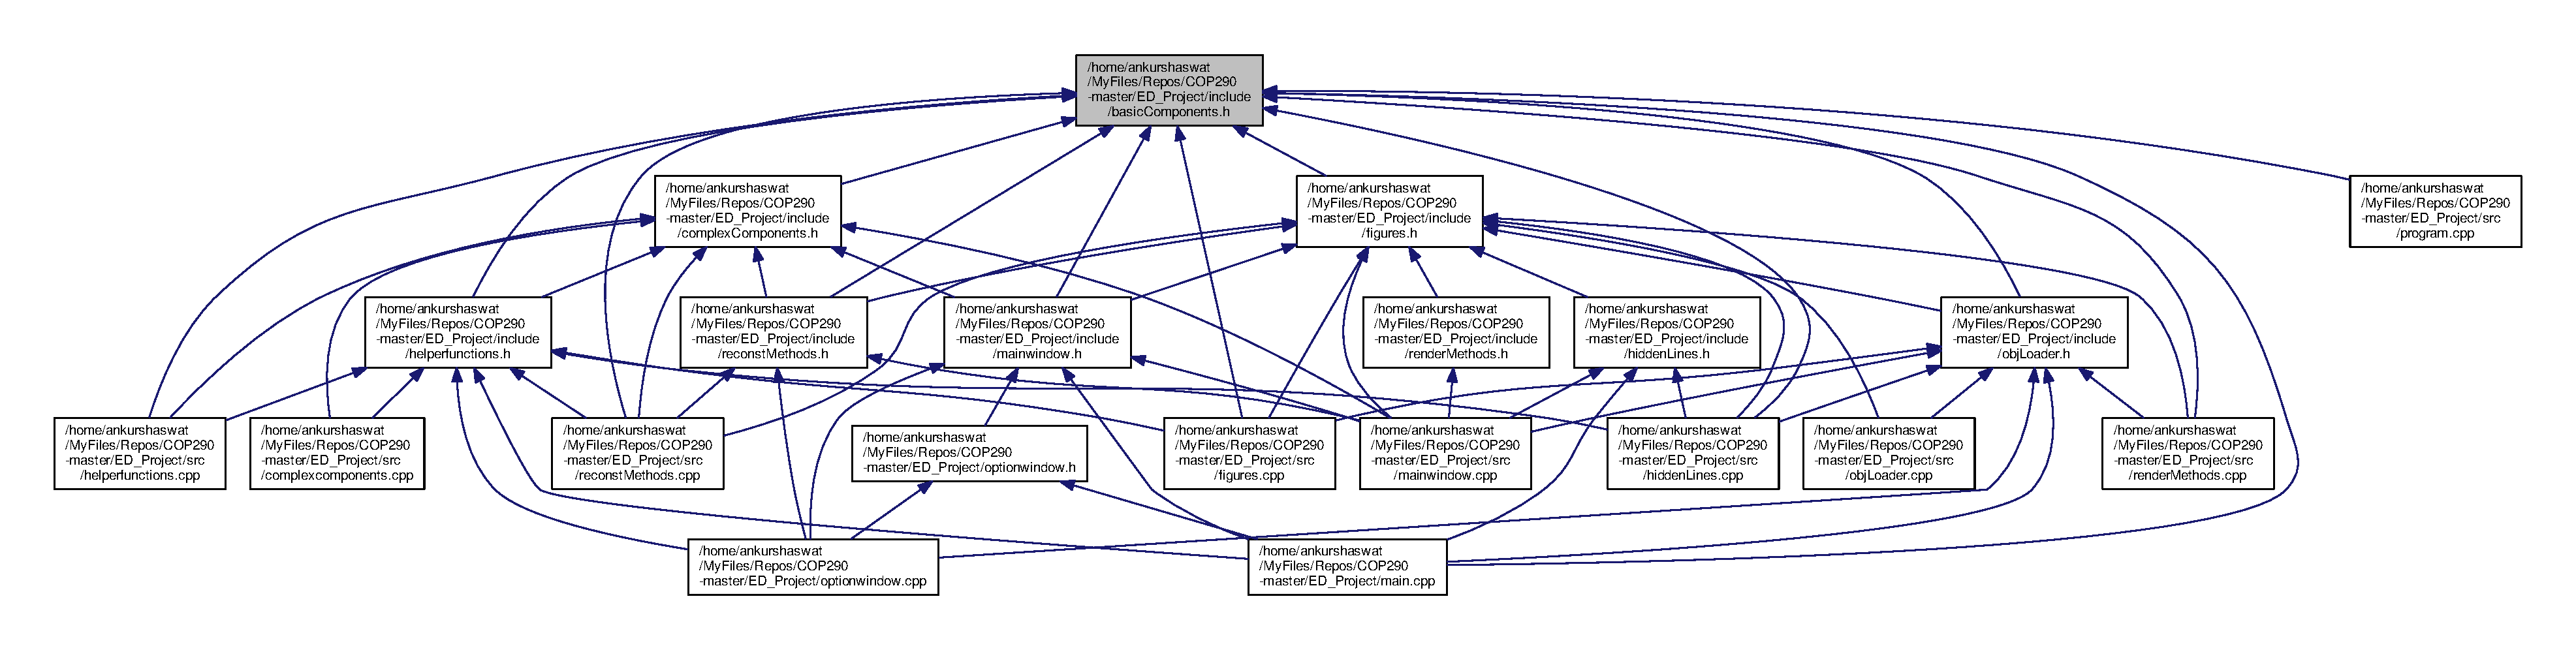
\includegraphics[width=350pt]{basicComponents_8h__dep__incl}
\end{center}
\end{figure}
\subsection*{Classes}
\begin{DoxyCompactItemize}
\item 
class \hyperlink{classVertice}{Vertice}
\end{DoxyCompactItemize}
\subsection*{Variables}
\begin{DoxyCompactItemize}
\item 
class \hyperlink{classVertice}{Vertice} \hyperlink{basicComponents_8h_a9e0e705b8112107f578dafc26a057db1}{edge} \mbox{[}10\mbox{]}
\item 
\hyperlink{classVertice}{Vertice} \hyperlink{basicComponents_8h_a5fb31efa54dedf5bd0e6301985a0af57}{vertice} \mbox{[}10\mbox{]}
\end{DoxyCompactItemize}


\subsection{Variable Documentation}
\mbox{\Hypertarget{basicComponents_8h_a9e0e705b8112107f578dafc26a057db1}\label{basicComponents_8h_a9e0e705b8112107f578dafc26a057db1}} 
\index{basic\+Components.\+h@{basic\+Components.\+h}!edge@{edge}}
\index{edge@{edge}!basic\+Components.\+h@{basic\+Components.\+h}}
\subsubsection{\texorpdfstring{edge}{edge}}
{\footnotesize\ttfamily class \hyperlink{classVertice}{Vertice} edge\mbox{[}10\mbox{]}}

\mbox{\Hypertarget{basicComponents_8h_a5fb31efa54dedf5bd0e6301985a0af57}\label{basicComponents_8h_a5fb31efa54dedf5bd0e6301985a0af57}} 
\index{basic\+Components.\+h@{basic\+Components.\+h}!vertice@{vertice}}
\index{vertice@{vertice}!basic\+Components.\+h@{basic\+Components.\+h}}
\subsubsection{\texorpdfstring{vertice}{vertice}}
{\footnotesize\ttfamily \hyperlink{classVertice}{Vertice} vertice\mbox{[}10\mbox{]}}


\hypertarget{complexComponents_8h}{}\section{/home/ankurshaswat/\+My\+Files/\+Repos/\+C\+O\+P290/\+Project1/\+Code/include/module1/complex\+Components.h File Reference}
\label{complexComponents_8h}\index{/home/ankurshaswat/\+My\+Files/\+Repos/\+C\+O\+P290/\+Project1/\+Code/include/module1/complex\+Components.\+h@{/home/ankurshaswat/\+My\+Files/\+Repos/\+C\+O\+P290/\+Project1/\+Code/include/module1/complex\+Components.\+h}}
{\ttfamily \#include \char`\"{}basic\+Components.\+h\char`\"{}}\newline
Include dependency graph for complex\+Components.\+h\+:\nopagebreak
\begin{figure}[H]
\begin{center}
\leavevmode
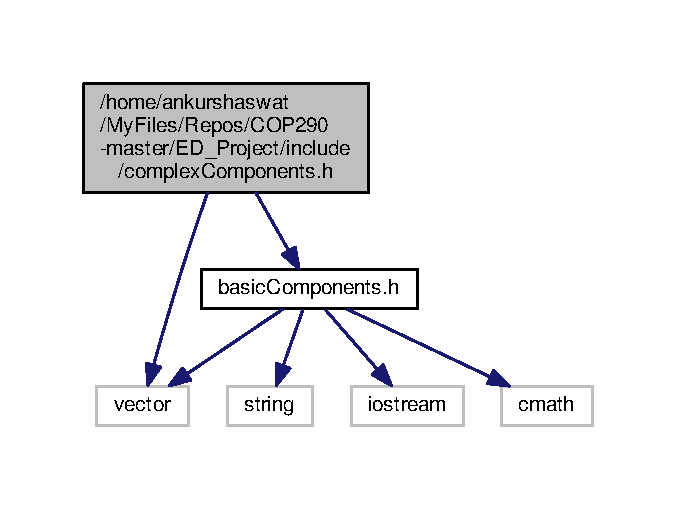
\includegraphics[width=240pt]{complexComponents_8h__incl}
\end{center}
\end{figure}
This graph shows which files directly or indirectly include this file\+:\nopagebreak
\begin{figure}[H]
\begin{center}
\leavevmode
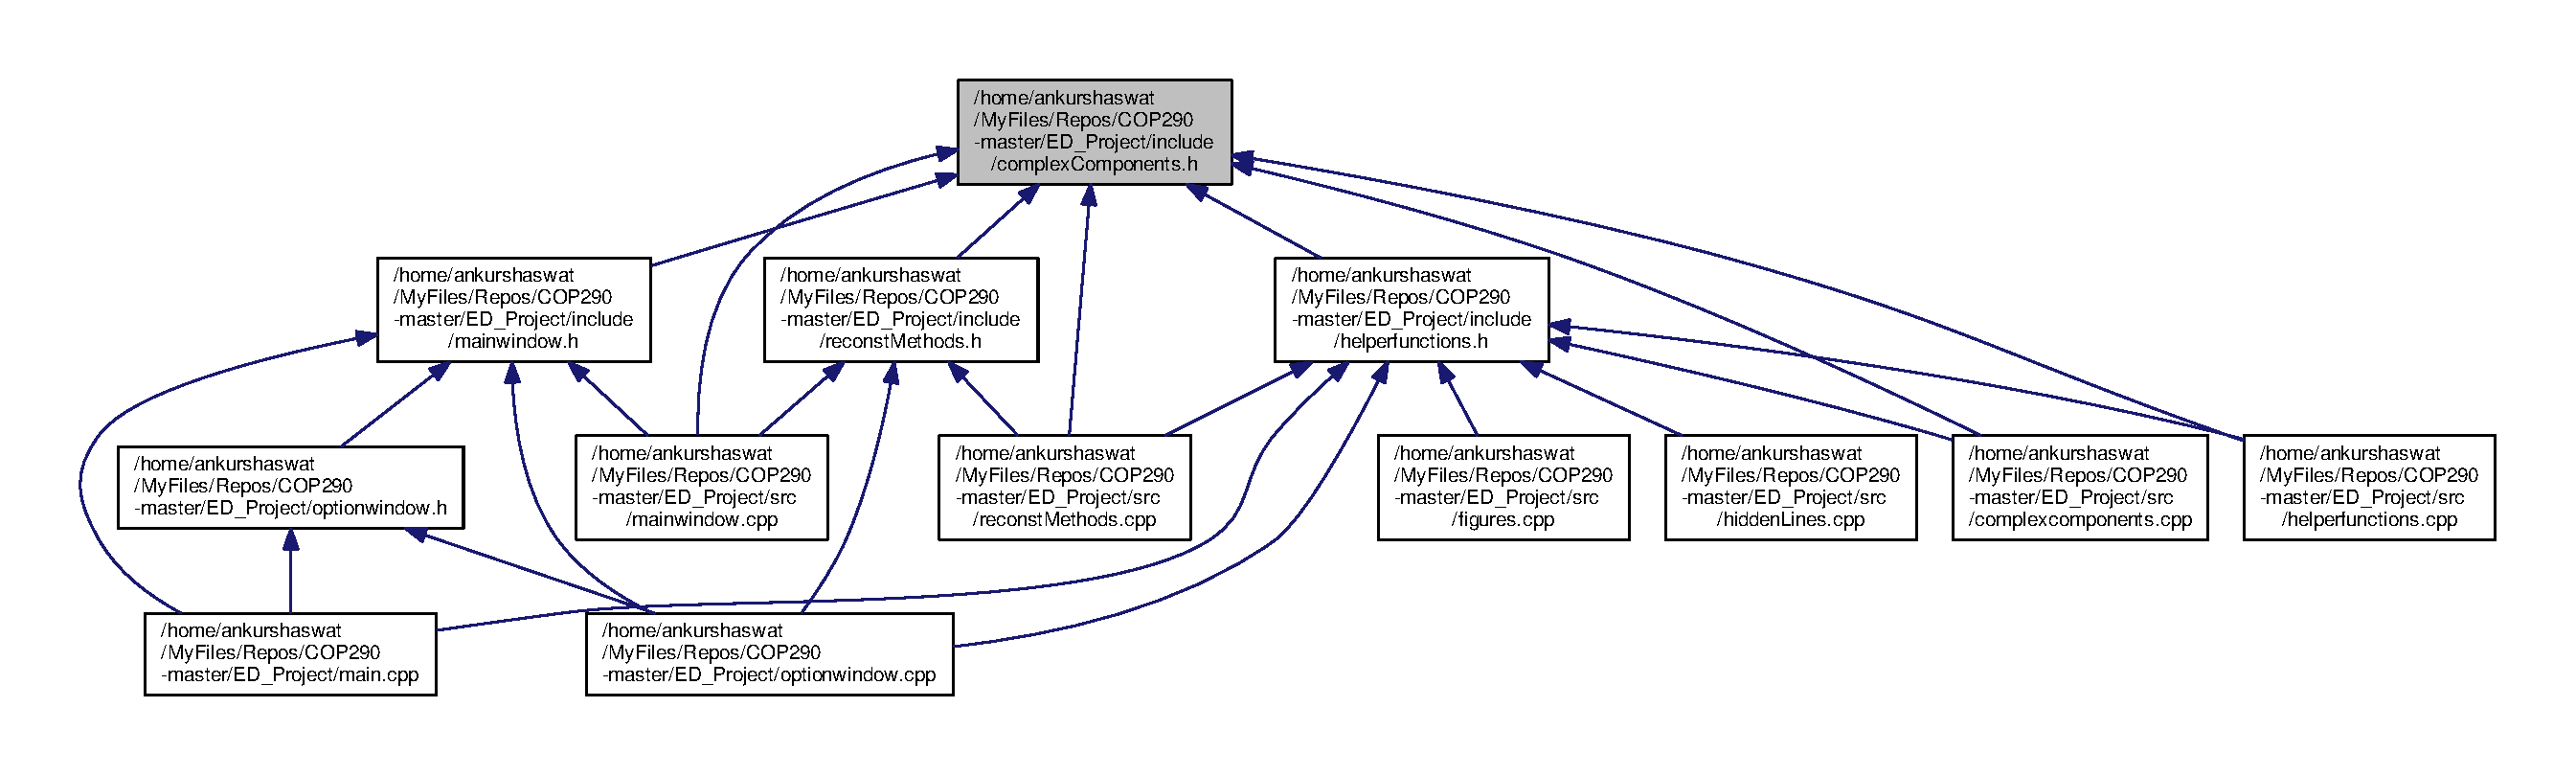
\includegraphics[width=240pt]{complexComponents_8h__dep__incl}
\end{center}
\end{figure}
\subsection*{Classes}
\begin{DoxyCompactItemize}
\item 
class \hyperlink{classEdgeLoop}{Edge\+Loop}
\item 
class \hyperlink{classWireFrame}{Wire\+Frame}
\end{DoxyCompactItemize}

\hypertarget{figures_8h}{}\section{/home/ankurshaswat/\+My\+Files/\+Repos/\+C\+O\+P290/\+Project1/\+Code/include/module1/figures.h File Reference}
\label{figures_8h}\index{/home/ankurshaswat/\+My\+Files/\+Repos/\+C\+O\+P290/\+Project1/\+Code/include/module1/figures.\+h@{/home/ankurshaswat/\+My\+Files/\+Repos/\+C\+O\+P290/\+Project1/\+Code/include/module1/figures.\+h}}
{\ttfamily \#include \char`\"{}basic\+Components.\+h\char`\"{}}\newline
Include dependency graph for figures.\+h\+:
\nopagebreak
\begin{figure}[H]
\begin{center}
\leavevmode
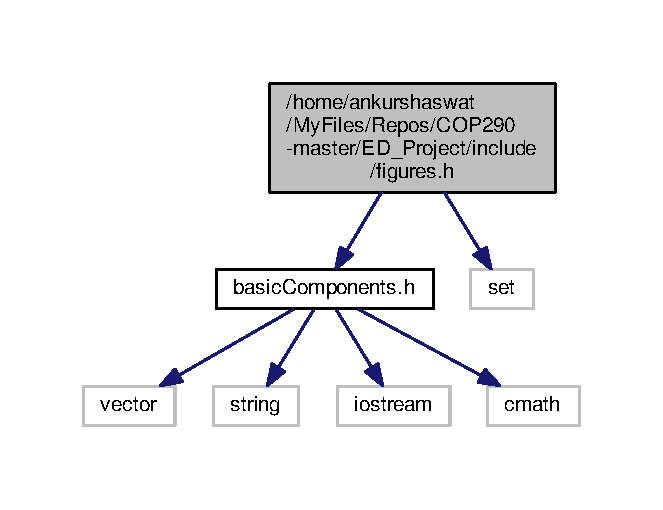
\includegraphics[width=206pt]{figures_8h__incl}
\end{center}
\end{figure}
This graph shows which files directly or indirectly include this file\+:
\nopagebreak
\begin{figure}[H]
\begin{center}
\leavevmode
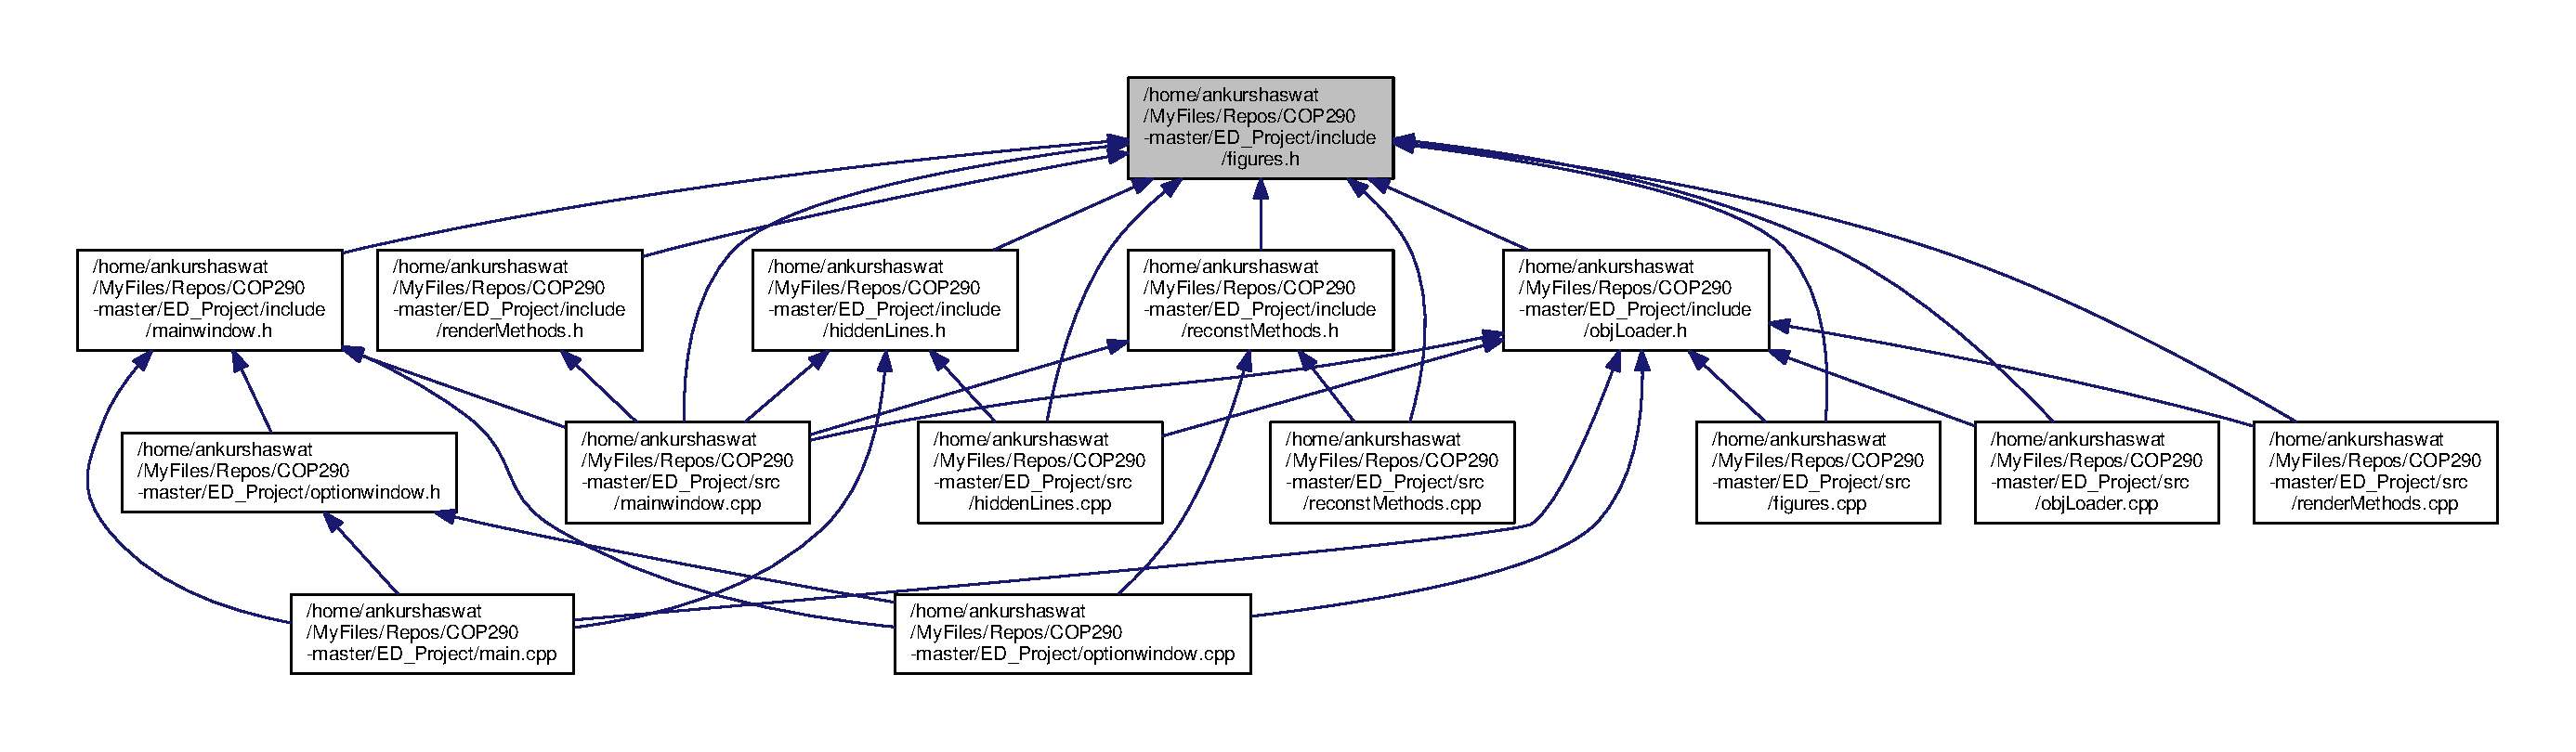
\includegraphics[width=350pt]{figures_8h__dep__incl}
\end{center}
\end{figure}

\hypertarget{helperfunctions_8h}{}\section{/home/ankurshaswat/\+My\+Files/\+Repos/\+C\+O\+P290-\/master/\+E\+D\+\_\+\+Project/include/helperfunctions.h File Reference}
\label{helperfunctions_8h}\index{/home/ankurshaswat/\+My\+Files/\+Repos/\+C\+O\+P290-\/master/\+E\+D\+\_\+\+Project/include/helperfunctions.\+h@{/home/ankurshaswat/\+My\+Files/\+Repos/\+C\+O\+P290-\/master/\+E\+D\+\_\+\+Project/include/helperfunctions.\+h}}
{\ttfamily \#include \char`\"{}basic\+Components.\+h\char`\"{}}\newline
{\ttfamily \#include \char`\"{}complex\+Components.\+h\char`\"{}}\newline
{\ttfamily \#include $<$vector$>$}\newline
{\ttfamily \#include $<$set$>$}\newline
Include dependency graph for helperfunctions.\+h\+:
\nopagebreak
\begin{figure}[H]
\begin{center}
\leavevmode
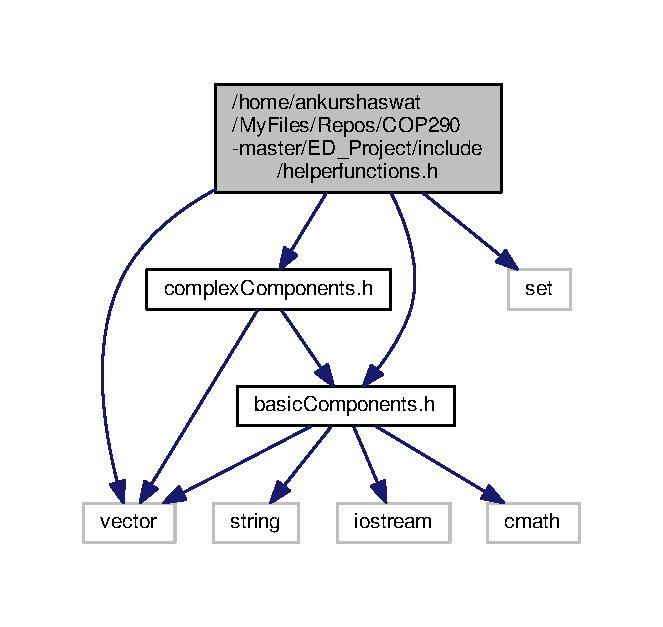
\includegraphics[width=318pt]{helperfunctions_8h__incl}
\end{center}
\end{figure}
This graph shows which files directly or indirectly include this file\+:
\nopagebreak
\begin{figure}[H]
\begin{center}
\leavevmode
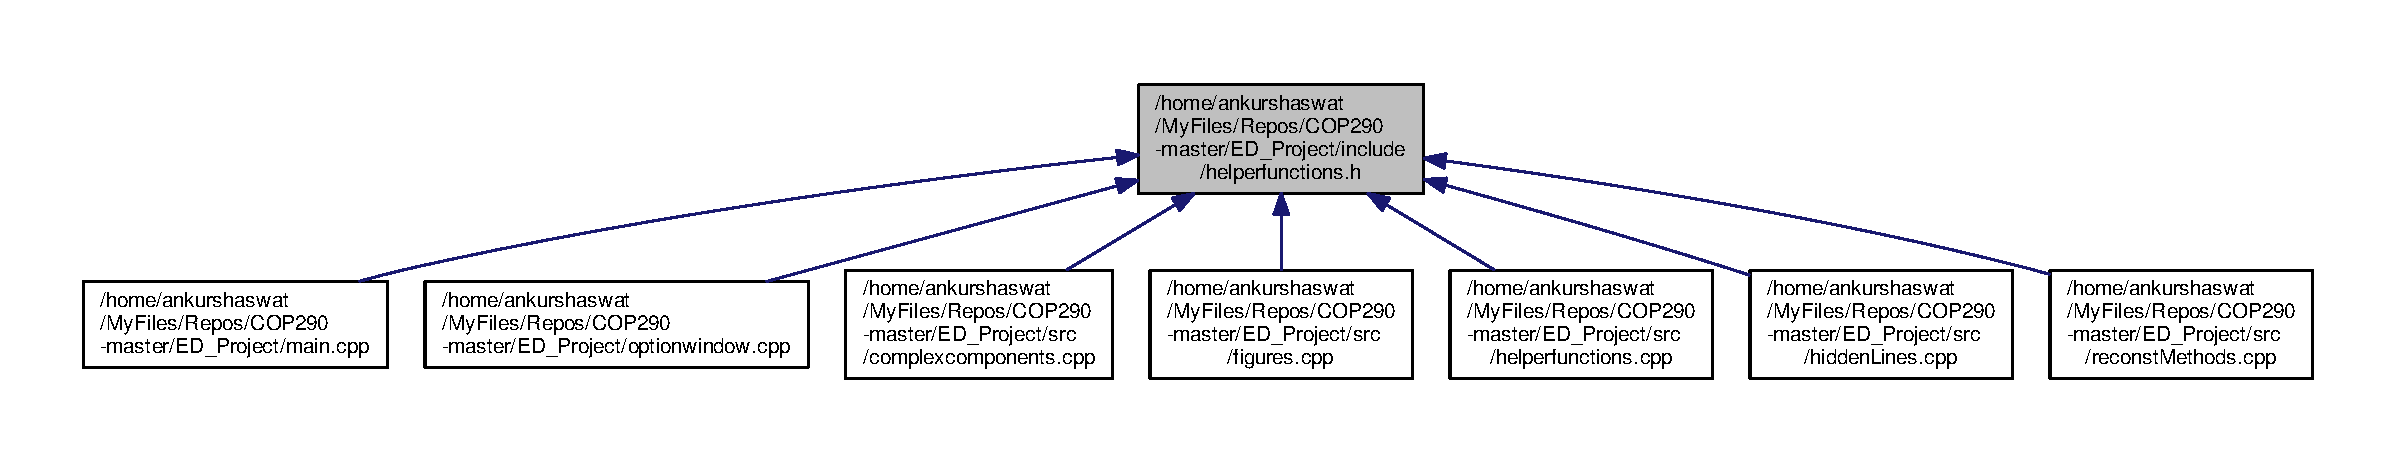
\includegraphics[width=350pt]{helperfunctions_8h__dep__incl}
\end{center}
\end{figure}
\subsection*{Functions}
\begin{DoxyCompactItemize}
\item 
\hyperlink{structVertice}{Vertice} \hyperlink{helperfunctions_8h_a4a9bde2a0de0b0199de919d3b4628e89}{transform} (\hyperlink{structVertice}{Vertice} v\+\_\+in, double Xrot, double Yrot, double Zrot, double Xoff, double Yoff, double Zoff)
\begin{DoxyCompactList}\small\item\em Transforms a vertice (rotation and offset) using matrix multiplication and returns a new \hyperlink{structVertice}{Vertice} object. \end{DoxyCompactList}\item 
pair$<$ int, \hyperlink{structVertice}{Vertice} $>$ \hyperlink{helperfunctions_8h_aeeffe6b314e92051412034d7e06b03d6}{get\+\_\+intersection} (\hyperlink{structEdge}{Edge} a, \hyperlink{structEdge}{Edge} b)
\begin{DoxyCompactList}\small\item\em Finds intersection of two edges (line segments) and also returns error if intersection does not exist. \end{DoxyCompactList}\item 
bool \hyperlink{helperfunctions_8h_a948ecdee044f4ebf6f132257557292fc}{is\+\_\+inside} (\hyperlink{structVertice}{Vertice} v, set$<$ \hyperlink{structEdge}{Edge} $>$ edge\+Set)
\begin{DoxyCompactList}\small\item\em Checks whether a vertice is inside (in 2d) of a face formed by an edge loop. \end{DoxyCompactList}\item 
bool \hyperlink{helperfunctions_8h_ab52930079ad22c64677a4bcafd8728c7}{is\+Subset} (vector$<$ int $>$ \&a, vector$<$ int $>$ \&b)
\item 
int \hyperlink{helperfunctions_8h_aaa98082eb9298793e9b30843abb80b6a}{vertice\+Present} (vector$<$ \hyperlink{structVertice}{Vertice} $>$ \&a, \hyperlink{structVertice}{Vertice} b)
\begin{DoxyCompactList}\small\item\em Checks if a vertice is present in a vector of vertices. \end{DoxyCompactList}\item 
\hyperlink{classWireFrame}{Wire\+Frame} \hyperlink{helperfunctions_8h_a9bcea272ffd067ba2d045be1af40cedf}{modify\+Wireframe} (\hyperlink{classWireFrame}{Wire\+Frame} wf, \hyperlink{structVertice}{Vertice} v)
\begin{DoxyCompactList}\small\item\em Takes a wireframe and subtracts coordinates of v from all its edge vertices. \end{DoxyCompactList}\end{DoxyCompactItemize}


\subsection{Function Documentation}
\mbox{\Hypertarget{helperfunctions_8h_aeeffe6b314e92051412034d7e06b03d6}\label{helperfunctions_8h_aeeffe6b314e92051412034d7e06b03d6}} 
\index{helperfunctions.\+h@{helperfunctions.\+h}!get\+\_\+intersection@{get\+\_\+intersection}}
\index{get\+\_\+intersection@{get\+\_\+intersection}!helperfunctions.\+h@{helperfunctions.\+h}}
\subsubsection{\texorpdfstring{get\+\_\+intersection()}{get\_intersection()}}
{\footnotesize\ttfamily pair$<$int,\hyperlink{structVertice}{Vertice}$>$ get\+\_\+intersection (\begin{DoxyParamCaption}\item[{\hyperlink{structEdge}{Edge}}]{a,  }\item[{\hyperlink{structEdge}{Edge}}]{b }\end{DoxyParamCaption})}



Finds intersection of two edges (line segments) and also returns error if intersection does not exist. 

returns (1,point of intersection) if intersecting, (0,\+\_\+) if overlapping and (-\/1,\+\_\+) if parallel Both edges are 2D edges \mbox{\Hypertarget{helperfunctions_8h_a948ecdee044f4ebf6f132257557292fc}\label{helperfunctions_8h_a948ecdee044f4ebf6f132257557292fc}} 
\index{helperfunctions.\+h@{helperfunctions.\+h}!is\+\_\+inside@{is\+\_\+inside}}
\index{is\+\_\+inside@{is\+\_\+inside}!helperfunctions.\+h@{helperfunctions.\+h}}
\subsubsection{\texorpdfstring{is\+\_\+inside()}{is\_inside()}}
{\footnotesize\ttfamily bool is\+\_\+inside (\begin{DoxyParamCaption}\item[{\hyperlink{structVertice}{Vertice}}]{v,  }\item[{set$<$ \hyperlink{structEdge}{Edge} $>$}]{edge\+Set }\end{DoxyParamCaption})}



Checks whether a vertice is inside (in 2d) of a face formed by an edge loop. 

Checks if vertex is inside the polygon defined by the edge set \mbox{\Hypertarget{helperfunctions_8h_ab52930079ad22c64677a4bcafd8728c7}\label{helperfunctions_8h_ab52930079ad22c64677a4bcafd8728c7}} 
\index{helperfunctions.\+h@{helperfunctions.\+h}!is\+Subset@{is\+Subset}}
\index{is\+Subset@{is\+Subset}!helperfunctions.\+h@{helperfunctions.\+h}}
\subsubsection{\texorpdfstring{is\+Subset()}{isSubset()}}
{\footnotesize\ttfamily bool is\+Subset (\begin{DoxyParamCaption}\item[{vector$<$ int $>$ \&}]{a,  }\item[{vector$<$ int $>$ \&}]{b }\end{DoxyParamCaption})}

A simple helper function to check if a is a subset of b \mbox{\Hypertarget{helperfunctions_8h_a9bcea272ffd067ba2d045be1af40cedf}\label{helperfunctions_8h_a9bcea272ffd067ba2d045be1af40cedf}} 
\index{helperfunctions.\+h@{helperfunctions.\+h}!modify\+Wireframe@{modify\+Wireframe}}
\index{modify\+Wireframe@{modify\+Wireframe}!helperfunctions.\+h@{helperfunctions.\+h}}
\subsubsection{\texorpdfstring{modify\+Wireframe()}{modifyWireframe()}}
{\footnotesize\ttfamily \hyperlink{classWireFrame}{Wire\+Frame} modify\+Wireframe (\begin{DoxyParamCaption}\item[{\hyperlink{classWireFrame}{Wire\+Frame}}]{wf,  }\item[{\hyperlink{structVertice}{Vertice}}]{v }\end{DoxyParamCaption})}



Takes a wireframe and subtracts coordinates of v from all its edge vertices. 

\mbox{\Hypertarget{helperfunctions_8h_a4a9bde2a0de0b0199de919d3b4628e89}\label{helperfunctions_8h_a4a9bde2a0de0b0199de919d3b4628e89}} 
\index{helperfunctions.\+h@{helperfunctions.\+h}!transform@{transform}}
\index{transform@{transform}!helperfunctions.\+h@{helperfunctions.\+h}}
\subsubsection{\texorpdfstring{transform()}{transform()}}
{\footnotesize\ttfamily \hyperlink{structVertice}{Vertice} transform (\begin{DoxyParamCaption}\item[{\hyperlink{structVertice}{Vertice}}]{v\+\_\+in,  }\item[{double}]{Xrot,  }\item[{double}]{Yrot,  }\item[{double}]{Zrot,  }\item[{double}]{Xoff,  }\item[{double}]{Yoff,  }\item[{double}]{Zoff }\end{DoxyParamCaption})}



Transforms a vertice (rotation and offset) using matrix multiplication and returns a new \hyperlink{structVertice}{Vertice} object. 

get transformed 3D object \mbox{\Hypertarget{helperfunctions_8h_aaa98082eb9298793e9b30843abb80b6a}\label{helperfunctions_8h_aaa98082eb9298793e9b30843abb80b6a}} 
\index{helperfunctions.\+h@{helperfunctions.\+h}!vertice\+Present@{vertice\+Present}}
\index{vertice\+Present@{vertice\+Present}!helperfunctions.\+h@{helperfunctions.\+h}}
\subsubsection{\texorpdfstring{vertice\+Present()}{verticePresent()}}
{\footnotesize\ttfamily int vertice\+Present (\begin{DoxyParamCaption}\item[{vector$<$ \hyperlink{structVertice}{Vertice} $>$ \&}]{a,  }\item[{\hyperlink{structVertice}{Vertice}}]{b }\end{DoxyParamCaption})}



Checks if a vertice is present in a vector of vertices. 

A simple helper function which checks if vertex is already present in vector (allowing for some error correction) 
\hypertarget{hiddenLines_8h}{}\section{/home/ankurshaswat/\+My\+Files/\+Repos/\+C\+O\+P290/working\+\_\+3d\+\_\+to\+\_\+2d/include/module1/hidden\+Lines.h File Reference}
\label{hiddenLines_8h}\index{/home/ankurshaswat/\+My\+Files/\+Repos/\+C\+O\+P290/working\+\_\+3d\+\_\+to\+\_\+2d/include/module1/hidden\+Lines.\+h@{/home/ankurshaswat/\+My\+Files/\+Repos/\+C\+O\+P290/working\+\_\+3d\+\_\+to\+\_\+2d/include/module1/hidden\+Lines.\+h}}
{\ttfamily \#include $<$Qt\+Ui\+Tools$>$}\newline
{\ttfamily \#include \char`\"{}figures.\+h\char`\"{}}\newline
Include dependency graph for hidden\+Lines.\+h\+:
\nopagebreak
\begin{figure}[H]
\begin{center}
\leavevmode
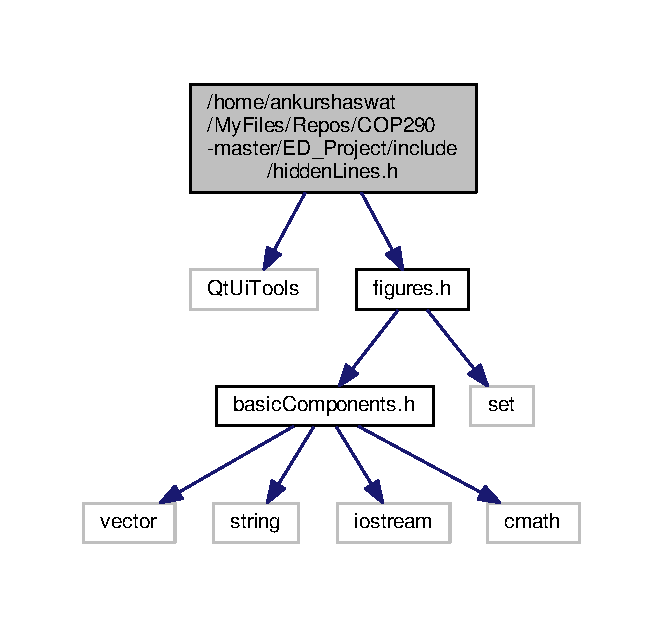
\includegraphics[width=318pt]{hiddenLines_8h__incl}
\end{center}
\end{figure}
This graph shows which files directly or indirectly include this file\+:
\nopagebreak
\begin{figure}[H]
\begin{center}
\leavevmode
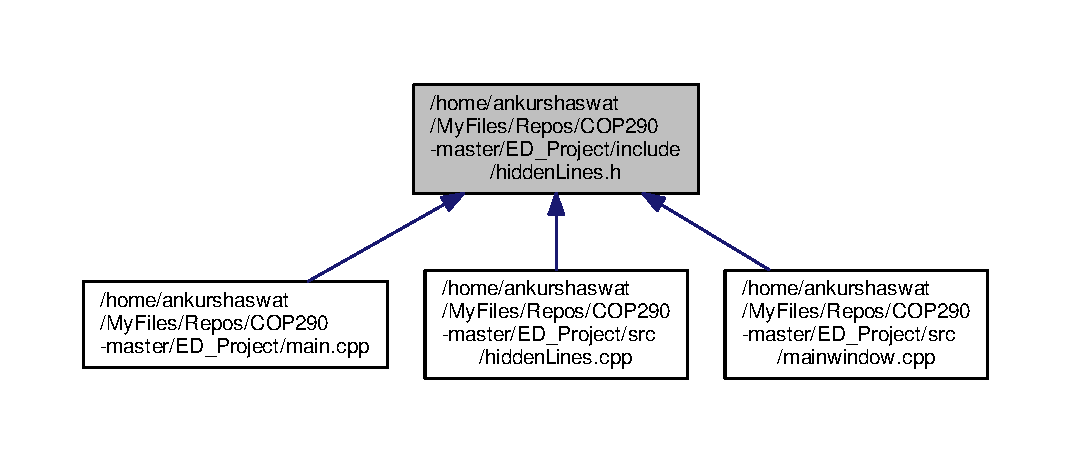
\includegraphics[width=350pt]{hiddenLines_8h__dep__incl}
\end{center}
\end{figure}
\subsection*{Macros}
\begin{DoxyCompactItemize}
\item 
\#define \hyperlink{hiddenLines_8h_a6e8530b9723b50941eb061538be8def3}{R\+E\+N\+D\+E\+R\+M\+E\+T\+H\+O\+D\+S\+\_\+H}
\end{DoxyCompactItemize}
\subsection*{Functions}
\begin{DoxyCompactItemize}
\item 
void \hyperlink{hiddenLines_8h_aafdedb0fe0862c4196f86c1c1828d27f}{render2\+D\+Hidden} (\hyperlink{classFig3D}{Fig3D} \&object3D, Q\+Painter \&painter, int plane)
\begin{DoxyCompactList}\small\item\em Renders the figure and also marks lines as hidden where they are hidden by some plane. \end{DoxyCompactList}\item 
bool \hyperlink{hiddenLines_8h_a75204ad0589a339061889fd407aa38e2}{opposite\+\_\+side} (vector$<$ \hyperlink{structVertice}{Vertice} $>$ \&face\+Vertices, \hyperlink{structVertice}{Vertice} a, \hyperlink{structVertice}{Vertice} b)
\item 
\hyperlink{structVertice}{Vertice} \hyperlink{hiddenLines_8h_a5245c9f2d3321def89057b7d397d84e3}{back\+\_\+proj} (\hyperlink{structVertice}{Vertice} v, \hyperlink{structEdge}{Edge} e, int plane)
\end{DoxyCompactItemize}


\subsection{Macro Definition Documentation}
\mbox{\Hypertarget{hiddenLines_8h_a6e8530b9723b50941eb061538be8def3}\label{hiddenLines_8h_a6e8530b9723b50941eb061538be8def3}} 
\index{hidden\+Lines.\+h@{hidden\+Lines.\+h}!R\+E\+N\+D\+E\+R\+M\+E\+T\+H\+O\+D\+S\+\_\+H@{R\+E\+N\+D\+E\+R\+M\+E\+T\+H\+O\+D\+S\+\_\+H}}
\index{R\+E\+N\+D\+E\+R\+M\+E\+T\+H\+O\+D\+S\+\_\+H@{R\+E\+N\+D\+E\+R\+M\+E\+T\+H\+O\+D\+S\+\_\+H}!hidden\+Lines.\+h@{hidden\+Lines.\+h}}
\subsubsection{\texorpdfstring{R\+E\+N\+D\+E\+R\+M\+E\+T\+H\+O\+D\+S\+\_\+H}{RENDERMETHODS\_H}}
{\footnotesize\ttfamily \#define R\+E\+N\+D\+E\+R\+M\+E\+T\+H\+O\+D\+S\+\_\+H}

Methods for rendering 3D object and diplaying 2D views (will use Open\+GL and G\+TK libraries) 

\subsection{Function Documentation}
\mbox{\Hypertarget{hiddenLines_8h_a5245c9f2d3321def89057b7d397d84e3}\label{hiddenLines_8h_a5245c9f2d3321def89057b7d397d84e3}} 
\index{hidden\+Lines.\+h@{hidden\+Lines.\+h}!back\+\_\+proj@{back\+\_\+proj}}
\index{back\+\_\+proj@{back\+\_\+proj}!hidden\+Lines.\+h@{hidden\+Lines.\+h}}
\subsubsection{\texorpdfstring{back\+\_\+proj()}{back\_proj()}}
{\footnotesize\ttfamily \hyperlink{structVertice}{Vertice} back\+\_\+proj (\begin{DoxyParamCaption}\item[{\hyperlink{structVertice}{Vertice}}]{v,  }\item[{\hyperlink{structEdge}{Edge}}]{e,  }\item[{int}]{plane }\end{DoxyParamCaption})}

returns vertex on 3D edge e whose projection is v

returns 3D vertex on \hyperlink{structEdge}{Edge} e whose projection is v \mbox{\Hypertarget{hiddenLines_8h_a75204ad0589a339061889fd407aa38e2}\label{hiddenLines_8h_a75204ad0589a339061889fd407aa38e2}} 
\index{hidden\+Lines.\+h@{hidden\+Lines.\+h}!opposite\+\_\+side@{opposite\+\_\+side}}
\index{opposite\+\_\+side@{opposite\+\_\+side}!hidden\+Lines.\+h@{hidden\+Lines.\+h}}
\subsubsection{\texorpdfstring{opposite\+\_\+side()}{opposite\_side()}}
{\footnotesize\ttfamily bool opposite\+\_\+side (\begin{DoxyParamCaption}\item[{vector$<$ \hyperlink{structVertice}{Vertice} $>$ \&}]{face\+Vertices,  }\item[{\hyperlink{structVertice}{Vertice}}]{e,  }\item[{\hyperlink{structVertice}{Vertice}}]{f }\end{DoxyParamCaption})}

returns true if a and b are on opposite side of plane formed by face\+Vertices , false otherwise \mbox{\Hypertarget{hiddenLines_8h_aafdedb0fe0862c4196f86c1c1828d27f}\label{hiddenLines_8h_aafdedb0fe0862c4196f86c1c1828d27f}} 
\index{hidden\+Lines.\+h@{hidden\+Lines.\+h}!render2\+D\+Hidden@{render2\+D\+Hidden}}
\index{render2\+D\+Hidden@{render2\+D\+Hidden}!hidden\+Lines.\+h@{hidden\+Lines.\+h}}
\subsubsection{\texorpdfstring{render2\+D\+Hidden()}{render2DHidden()}}
{\footnotesize\ttfamily void render2\+D\+Hidden (\begin{DoxyParamCaption}\item[{\hyperlink{classFig3D}{Fig3D} \&}]{object3D,  }\item[{Q\+Painter \&}]{painter,  }\item[{int}]{plane }\end{DoxyParamCaption})}



Renders the figure and also marks lines as hidden where they are hidden by some plane. 


\hypertarget{mainwindow_8h}{}\section{/home/ankurshaswat/\+My\+Files/\+Repos/\+C\+O\+P290/working\+\_\+3d\+\_\+to\+\_\+2d/include/module1/mainwindow.h File Reference}
\label{mainwindow_8h}\index{/home/ankurshaswat/\+My\+Files/\+Repos/\+C\+O\+P290/working\+\_\+3d\+\_\+to\+\_\+2d/include/module1/mainwindow.\+h@{/home/ankurshaswat/\+My\+Files/\+Repos/\+C\+O\+P290/working\+\_\+3d\+\_\+to\+\_\+2d/include/module1/mainwindow.\+h}}
{\ttfamily \#include $<$Q\+Main\+Window$>$}\newline
{\ttfamily \#include \char`\"{}basic\+Components.\+h\char`\"{}}\newline
{\ttfamily \#include \char`\"{}figures.\+h\char`\"{}}\newline
{\ttfamily \#include \char`\"{}complex\+Components.\+h\char`\"{}}\newline
Include dependency graph for mainwindow.\+h\+:
\nopagebreak
\begin{figure}[H]
\begin{center}
\leavevmode
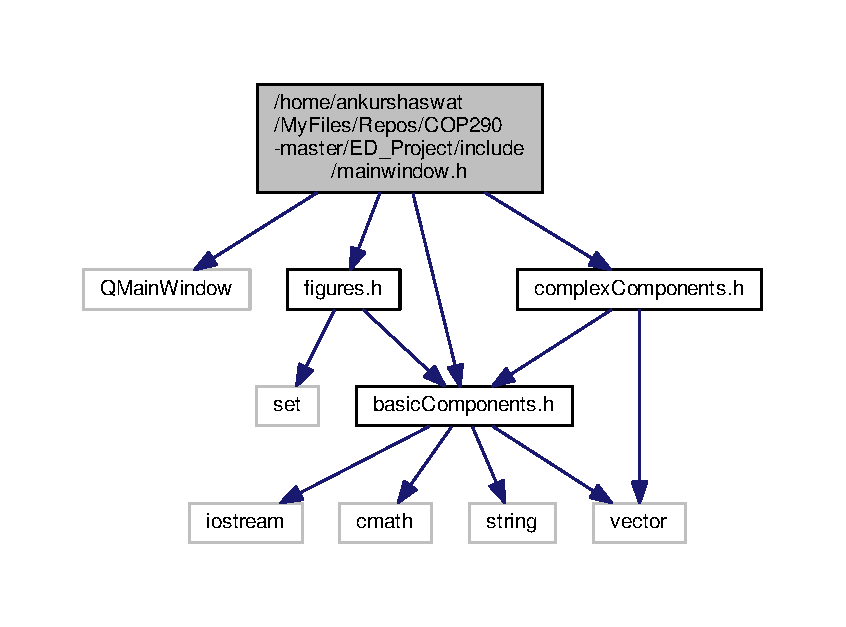
\includegraphics[width=350pt]{mainwindow_8h__incl}
\end{center}
\end{figure}
This graph shows which files directly or indirectly include this file\+:
\nopagebreak
\begin{figure}[H]
\begin{center}
\leavevmode
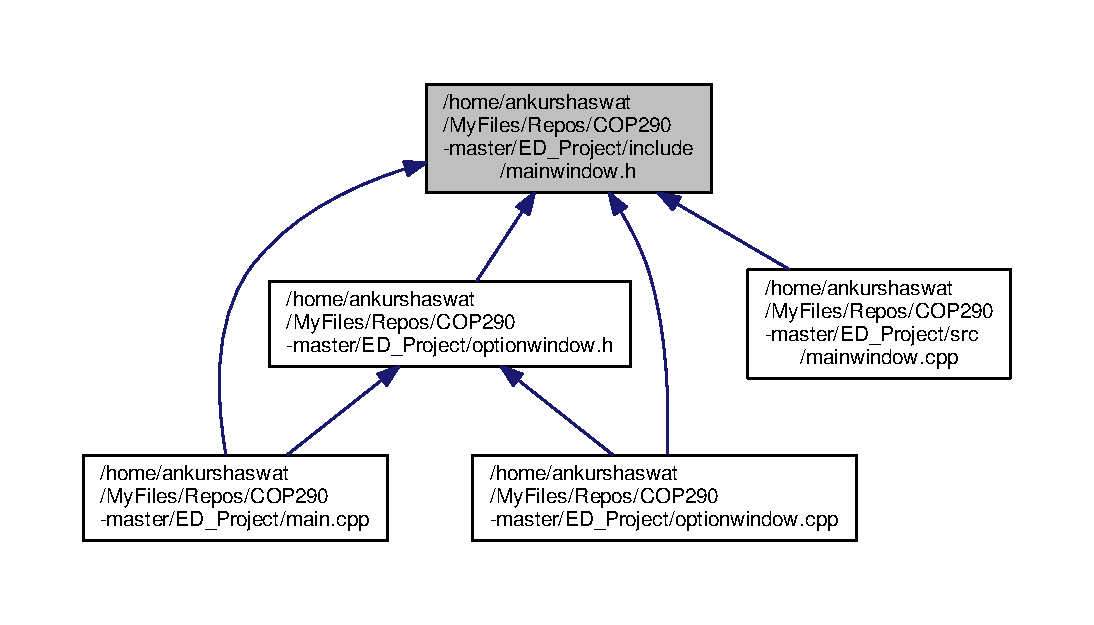
\includegraphics[width=350pt]{mainwindow_8h__dep__incl}
\end{center}
\end{figure}
\subsection*{Classes}
\begin{DoxyCompactItemize}
\item 
class \hyperlink{classMainWindow}{Main\+Window}
\end{DoxyCompactItemize}
\subsection*{Namespaces}
\begin{DoxyCompactItemize}
\item 
 \hyperlink{namespaceUi}{Ui}
\end{DoxyCompactItemize}

\hypertarget{objLoader_8h}{}\section{/home/ankurshaswat/\+My\+Files/\+Repos/\+C\+O\+P290-\/master/\+E\+D\+\_\+\+Project/include/obj\+Loader.h File Reference}
\label{objLoader_8h}\index{/home/ankurshaswat/\+My\+Files/\+Repos/\+C\+O\+P290-\/master/\+E\+D\+\_\+\+Project/include/obj\+Loader.\+h@{/home/ankurshaswat/\+My\+Files/\+Repos/\+C\+O\+P290-\/master/\+E\+D\+\_\+\+Project/include/obj\+Loader.\+h}}
{\ttfamily \#include $<$set$>$}\newline
{\ttfamily \#include $<$vector$>$}\newline
{\ttfamily \#include \char`\"{}basic\+Components.\+h\char`\"{}}\newline
{\ttfamily \#include \char`\"{}figures.\+h\char`\"{}}\newline
Include dependency graph for obj\+Loader.\+h\+:
\nopagebreak
\begin{figure}[H]
\begin{center}
\leavevmode
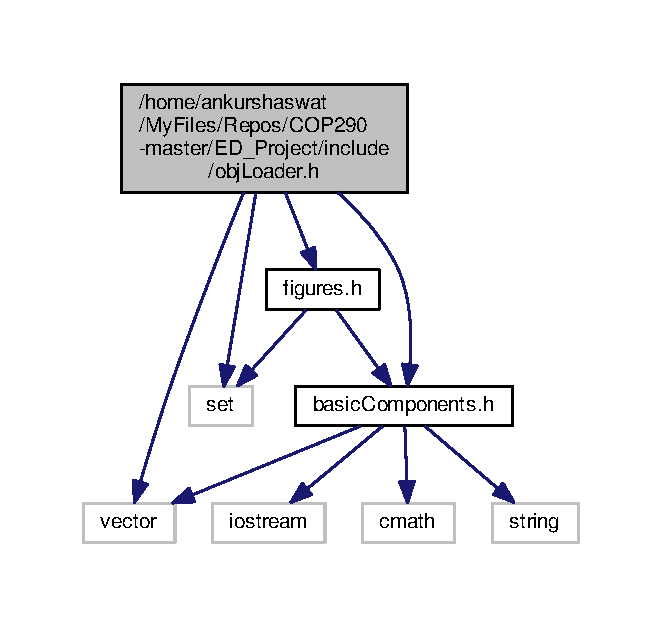
\includegraphics[width=318pt]{objLoader_8h__incl}
\end{center}
\end{figure}
This graph shows which files directly or indirectly include this file\+:
\nopagebreak
\begin{figure}[H]
\begin{center}
\leavevmode
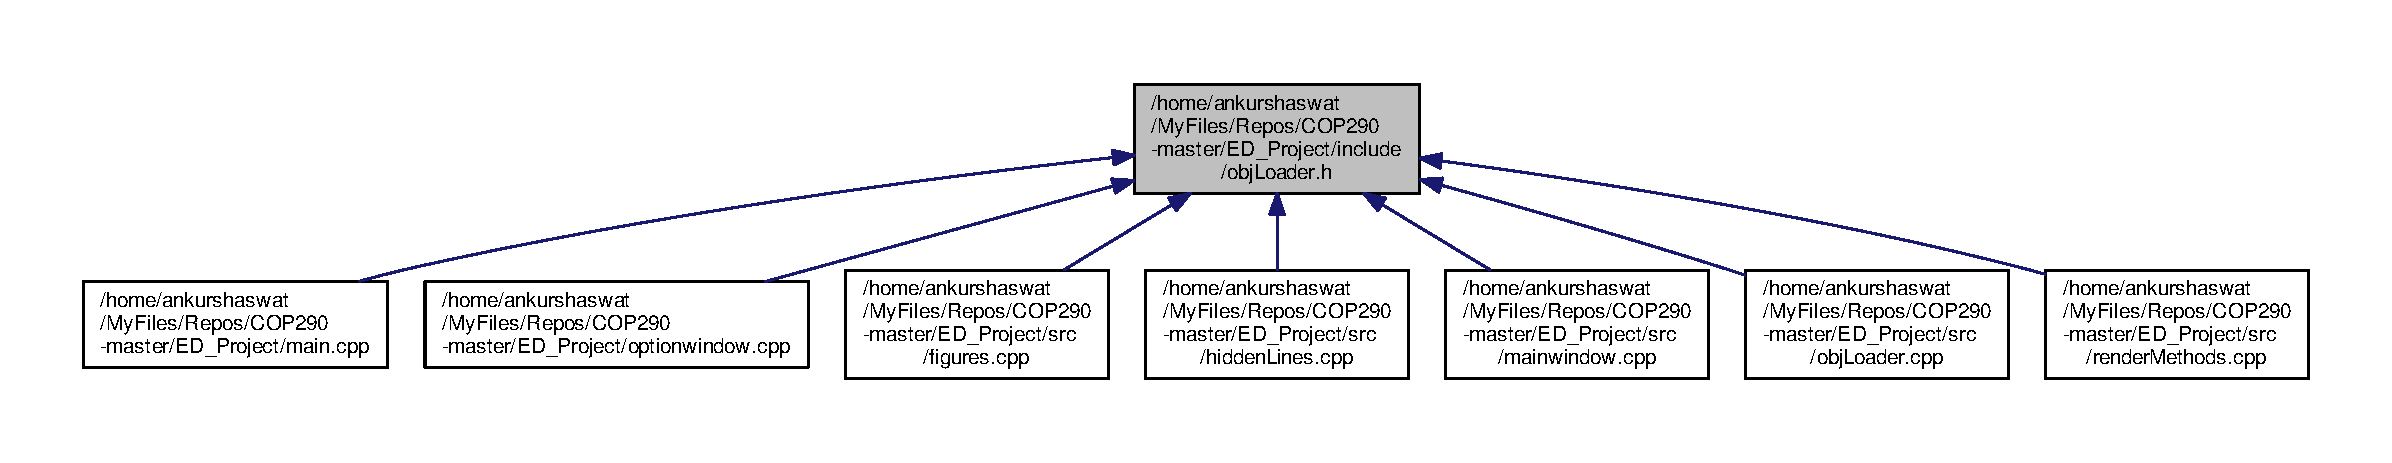
\includegraphics[width=350pt]{objLoader_8h__dep__incl}
\end{center}
\end{figure}
\subsection*{Functions}
\begin{DoxyCompactItemize}
\item 
\hyperlink{classFig3D}{Fig3D} \hyperlink{objLoader_8h_aceb7a3048c7f82ebf68f0256aedbe70f}{load\+O\+BJ} (const char $\ast$path)
\begin{DoxyCompactList}\small\item\em Function to load O\+BJ file and save its contents into a 3d figure object. \end{DoxyCompactList}\item 
bool \hyperlink{objLoader_8h_a6e505fb672d9a42fb27028c8340e2611}{get\+\_\+edges3D} (std\+::vector$<$ \hyperlink{structVertice}{Vertice} $>$ \&out\+\_\+vertices, std\+::vector$<$ std\+::vector$<$ unsigned int $>$ $>$ \&faces\+\_\+vertices, std\+::set$<$ \hyperlink{structEdge}{Edge} $>$ \&edge\+Set)
\end{DoxyCompactItemize}


\subsection{Function Documentation}
\mbox{\Hypertarget{objLoader_8h_a6e505fb672d9a42fb27028c8340e2611}\label{objLoader_8h_a6e505fb672d9a42fb27028c8340e2611}} 
\index{obj\+Loader.\+h@{obj\+Loader.\+h}!get\+\_\+edges3D@{get\+\_\+edges3D}}
\index{get\+\_\+edges3D@{get\+\_\+edges3D}!obj\+Loader.\+h@{obj\+Loader.\+h}}
\subsubsection{\texorpdfstring{get\+\_\+edges3\+D()}{get\_edges3D()}}
{\footnotesize\ttfamily bool get\+\_\+edges3D (\begin{DoxyParamCaption}\item[{std\+::vector$<$ \hyperlink{structVertice}{Vertice} $>$ \&}]{out\+\_\+vertices,  }\item[{std\+::vector$<$ std\+::vector$<$ unsigned int $>$ $>$ \&}]{faces\+\_\+vertices,  }\item[{std\+::set$<$ \hyperlink{structEdge}{Edge} $>$ \&}]{edge\+Set }\end{DoxyParamCaption})}

\mbox{\Hypertarget{objLoader_8h_aceb7a3048c7f82ebf68f0256aedbe70f}\label{objLoader_8h_aceb7a3048c7f82ebf68f0256aedbe70f}} 
\index{obj\+Loader.\+h@{obj\+Loader.\+h}!load\+O\+BJ@{load\+O\+BJ}}
\index{load\+O\+BJ@{load\+O\+BJ}!obj\+Loader.\+h@{obj\+Loader.\+h}}
\subsubsection{\texorpdfstring{load\+O\+B\+J()}{loadOBJ()}}
{\footnotesize\ttfamily \hyperlink{classFig3D}{Fig3D} load\+O\+BJ (\begin{DoxyParamCaption}\item[{const char $\ast$}]{path }\end{DoxyParamCaption})}



Function to load O\+BJ file and save its contents into a 3d figure object. 


\hypertarget{reconstMethods_8h}{}\section{/home/ankurshaswat/\+My\+Files/\+Repos/\+C\+O\+P290-\/master/\+E\+D\+\_\+\+Project/include/reconst\+Methods.h File Reference}
\label{reconstMethods_8h}\index{/home/ankurshaswat/\+My\+Files/\+Repos/\+C\+O\+P290-\/master/\+E\+D\+\_\+\+Project/include/reconst\+Methods.\+h@{/home/ankurshaswat/\+My\+Files/\+Repos/\+C\+O\+P290-\/master/\+E\+D\+\_\+\+Project/include/reconst\+Methods.\+h}}
{\ttfamily \#include \char`\"{}basic\+Components.\+h\char`\"{}}\newline
{\ttfamily \#include \char`\"{}complex\+Components.\+h\char`\"{}}\newline
{\ttfamily \#include \char`\"{}figures.\+h\char`\"{}}\newline
{\ttfamily \#include \char`\"{}structs.\+h\char`\"{}}\newline
Include dependency graph for reconst\+Methods.\+h\+:
\nopagebreak
\begin{figure}[H]
\begin{center}
\leavevmode
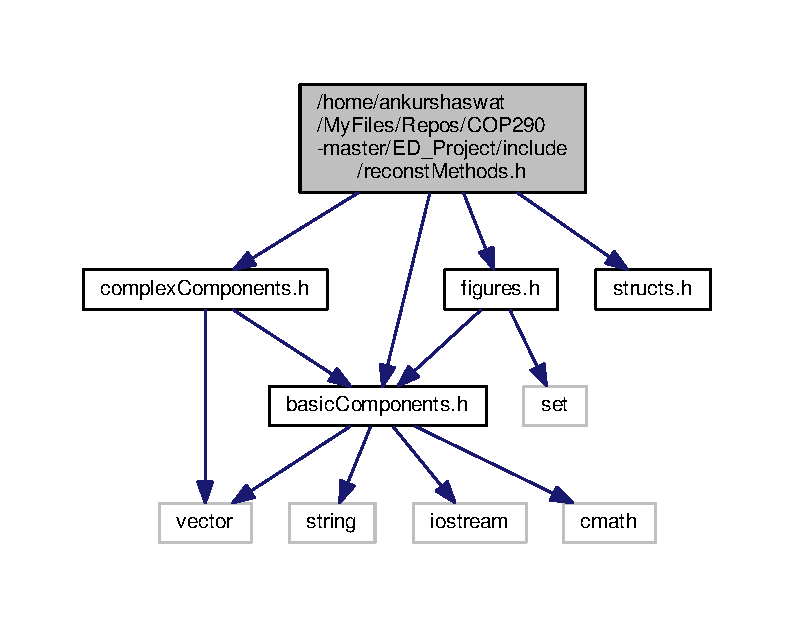
\includegraphics[width=350pt]{reconstMethods_8h__incl}
\end{center}
\end{figure}
This graph shows which files directly or indirectly include this file\+:
\nopagebreak
\begin{figure}[H]
\begin{center}
\leavevmode
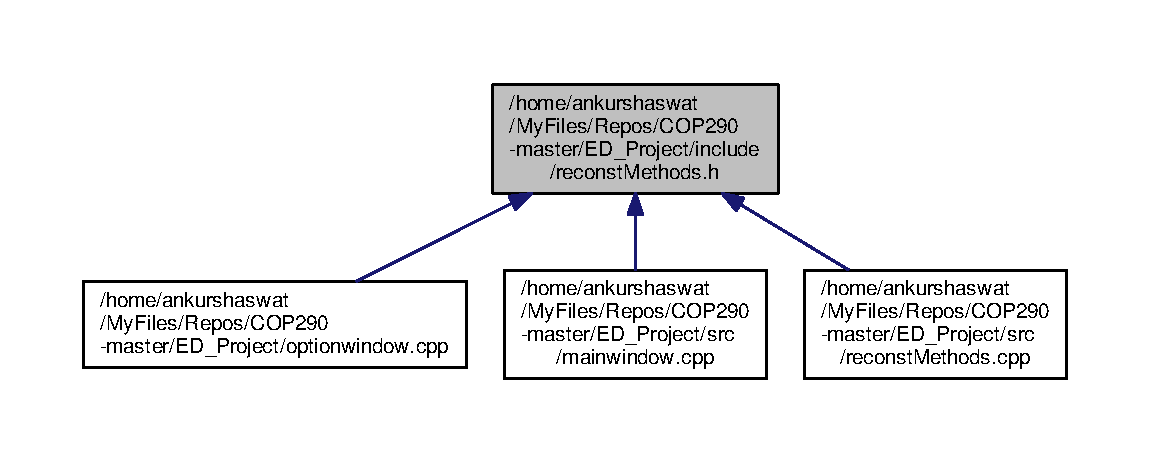
\includegraphics[width=350pt]{reconstMethods_8h__dep__incl}
\end{center}
\end{figure}
\subsection*{Functions}
\begin{DoxyCompactItemize}
\item 
\hyperlink{classWireFrame}{Wire\+Frame} \hyperlink{reconstMethods_8h_a110e71b7da4f490cc73c09b654d2db99}{const\+Uniq3d\+Edges} (vector$<$ vector$<$ \hyperlink{structEdge}{Edge} $>$ $>$ edge\+Set)
\begin{DoxyCompactList}\small\item\em Function to construct 3d edges from 2d edges by checking the possibility of the edges being projections of each other. \end{DoxyCompactList}\item 
std\+::vector$<$ std\+::vector$<$ \hyperlink{structEdge}{Edge} $>$ $>$ \hyperlink{reconstMethods_8h_ab5b36acd93691246a5e348eecc9225cf}{read\+File} (const char $\ast$)
\begin{DoxyCompactList}\small\item\em Function to read txt file contatining labelled data of xy , yz and xz views and returns the result as a vector of vector of edges. \end{DoxyCompactList}\item 
\hyperlink{classFig3D}{Fig3D} \hyperlink{reconstMethods_8h_a323870048d29be8ede27a7020e767c79}{wireframe\+To3D} (\hyperlink{classWireFrame}{Wire\+Frame} a)
\begin{DoxyCompactList}\small\item\em Takes a wireframe object and converts it into a 3d object by creating faces by forming edge loops. \end{DoxyCompactList}\item 
vector$<$ vector$<$ int $>$ $>$ \hyperlink{reconstMethods_8h_ad748b0dac80de637f972c4676f8ccdaa}{coplanar\+Edges} (vector$<$ \hyperlink{structEdge}{Edge} $>$ \&edges)
\item 
vector$<$ vector$<$ int $>$ $>$ \hyperlink{reconstMethods_8h_aed7e2db16ce5e7210f9f80b20a8af52f}{get\+Edge\+Loops} (vector$<$ \hyperlink{structEdge}{Edge} $>$ \&edges, vector$<$ int $>$ coplanar\+Indices)
\end{DoxyCompactItemize}


\subsection{Function Documentation}
\mbox{\Hypertarget{reconstMethods_8h_a110e71b7da4f490cc73c09b654d2db99}\label{reconstMethods_8h_a110e71b7da4f490cc73c09b654d2db99}} 
\index{reconst\+Methods.\+h@{reconst\+Methods.\+h}!const\+Uniq3d\+Edges@{const\+Uniq3d\+Edges}}
\index{const\+Uniq3d\+Edges@{const\+Uniq3d\+Edges}!reconst\+Methods.\+h@{reconst\+Methods.\+h}}
\subsubsection{\texorpdfstring{const\+Uniq3d\+Edges()}{constUniq3dEdges()}}
{\footnotesize\ttfamily \hyperlink{classWireFrame}{Wire\+Frame} const\+Uniq3d\+Edges (\begin{DoxyParamCaption}\item[{vector$<$ vector$<$ \hyperlink{structEdge}{Edge} $>$ $>$}]{edge\+Set }\end{DoxyParamCaption})}



Function to construct 3d edges from 2d edges by checking the possibility of the edges being projections of each other. 

Defines methods required for 3D reconstruction process \mbox{\Hypertarget{reconstMethods_8h_ad748b0dac80de637f972c4676f8ccdaa}\label{reconstMethods_8h_ad748b0dac80de637f972c4676f8ccdaa}} 
\index{reconst\+Methods.\+h@{reconst\+Methods.\+h}!coplanar\+Edges@{coplanar\+Edges}}
\index{coplanar\+Edges@{coplanar\+Edges}!reconst\+Methods.\+h@{reconst\+Methods.\+h}}
\subsubsection{\texorpdfstring{coplanar\+Edges()}{coplanarEdges()}}
{\footnotesize\ttfamily vector$<$ vector$<$int$>$ $>$ coplanar\+Edges (\begin{DoxyParamCaption}\item[{vector$<$ \hyperlink{structEdge}{Edge} $>$ \&}]{edges }\end{DoxyParamCaption})}

Returns coplanar sets of edges of size$>$=3 (each coplanar set is represented as a list of edge indices) \mbox{\Hypertarget{reconstMethods_8h_aed7e2db16ce5e7210f9f80b20a8af52f}\label{reconstMethods_8h_aed7e2db16ce5e7210f9f80b20a8af52f}} 
\index{reconst\+Methods.\+h@{reconst\+Methods.\+h}!get\+Edge\+Loops@{get\+Edge\+Loops}}
\index{get\+Edge\+Loops@{get\+Edge\+Loops}!reconst\+Methods.\+h@{reconst\+Methods.\+h}}
\subsubsection{\texorpdfstring{get\+Edge\+Loops()}{getEdgeLoops()}}
{\footnotesize\ttfamily vector$<$ vector$<$int$>$ $>$ get\+Edge\+Loops (\begin{DoxyParamCaption}\item[{vector$<$ \hyperlink{structEdge}{Edge} $>$ \&}]{edges,  }\item[{vector$<$ int $>$}]{coplanar\+Indices }\end{DoxyParamCaption})}

takes input a set of coplanar edges (as edges + indices) and returns a list of edge loops(candidate faces) formed using these edges (each edge\+Loop is represented by a list of indices) \mbox{\Hypertarget{reconstMethods_8h_ab5b36acd93691246a5e348eecc9225cf}\label{reconstMethods_8h_ab5b36acd93691246a5e348eecc9225cf}} 
\index{reconst\+Methods.\+h@{reconst\+Methods.\+h}!read\+File@{read\+File}}
\index{read\+File@{read\+File}!reconst\+Methods.\+h@{reconst\+Methods.\+h}}
\subsubsection{\texorpdfstring{read\+File()}{readFile()}}
{\footnotesize\ttfamily std\+::vector$<$std\+::vector$<$\hyperlink{structEdge}{Edge}$>$ $>$ read\+File (\begin{DoxyParamCaption}\item[{const char $\ast$}]{ }\end{DoxyParamCaption})}



Function to read txt file contatining labelled data of xy , yz and xz views and returns the result as a vector of vector of edges. 

\mbox{\Hypertarget{reconstMethods_8h_a323870048d29be8ede27a7020e767c79}\label{reconstMethods_8h_a323870048d29be8ede27a7020e767c79}} 
\index{reconst\+Methods.\+h@{reconst\+Methods.\+h}!wireframe\+To3D@{wireframe\+To3D}}
\index{wireframe\+To3D@{wireframe\+To3D}!reconst\+Methods.\+h@{reconst\+Methods.\+h}}
\subsubsection{\texorpdfstring{wireframe\+To3\+D()}{wireframeTo3D()}}
{\footnotesize\ttfamily \hyperlink{classFig3D}{Fig3D} wireframe\+To3D (\begin{DoxyParamCaption}\item[{\hyperlink{classWireFrame}{Wire\+Frame}}]{a }\end{DoxyParamCaption})}



Takes a wireframe object and converts it into a 3d object by creating faces by forming edge loops. 


\hypertarget{renderMethods_8h}{}\section{/home/ankurshaswat/\+My\+Files/\+Repos/\+C\+O\+P290-\/master/\+E\+D\+\_\+\+Project/include/render\+Methods.h File Reference}
\label{renderMethods_8h}\index{/home/ankurshaswat/\+My\+Files/\+Repos/\+C\+O\+P290-\/master/\+E\+D\+\_\+\+Project/include/render\+Methods.\+h@{/home/ankurshaswat/\+My\+Files/\+Repos/\+C\+O\+P290-\/master/\+E\+D\+\_\+\+Project/include/render\+Methods.\+h}}
{\ttfamily \#include $<$Qt\+Ui\+Tools$>$}\newline
{\ttfamily \#include \char`\"{}figures.\+h\char`\"{}}\newline
Include dependency graph for render\+Methods.\+h\+:
\nopagebreak
\begin{figure}[H]
\begin{center}
\leavevmode
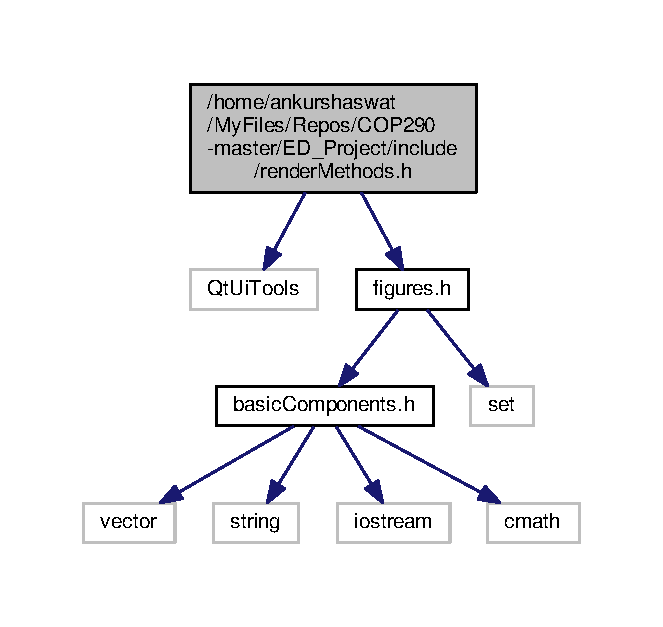
\includegraphics[width=318pt]{renderMethods_8h__incl}
\end{center}
\end{figure}
This graph shows which files directly or indirectly include this file\+:
\nopagebreak
\begin{figure}[H]
\begin{center}
\leavevmode
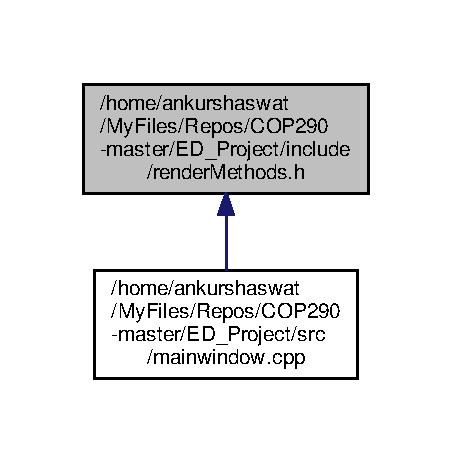
\includegraphics[width=217pt]{renderMethods_8h__dep__incl}
\end{center}
\end{figure}
\subsection*{Functions}
\begin{DoxyCompactItemize}
\item 
void \hyperlink{renderMethods_8h_ab6043f874ec8d70f6af6449bbf1ab02a}{render} (\hyperlink{classFig3D}{Fig3D} a)
\begin{DoxyCompactList}\small\item\em Function to render a 3d figure. \end{DoxyCompactList}\item 
void \hyperlink{renderMethods_8h_abbe049f22c313df9c0fe89db2a69f154}{render2D} (\hyperlink{classFig3D}{Fig3D} \&object3D, Q\+Painter \&painter, int plane)
\begin{DoxyCompactList}\small\item\em Function to render 2d views generated from 3d object. \end{DoxyCompactList}\item 
void \hyperlink{renderMethods_8h_a75faaca4675cd8cd28ae49e79c140c42}{render\+Axes} (\hyperlink{classFig3D}{Fig3D} \&object3D, Q\+Painter \&painter, int plane, double scale\+\_\+factor)
\begin{DoxyCompactList}\small\item\em Function to display axes on the labels for reference. \end{DoxyCompactList}\end{DoxyCompactItemize}


\subsection{Function Documentation}
\mbox{\Hypertarget{renderMethods_8h_ab6043f874ec8d70f6af6449bbf1ab02a}\label{renderMethods_8h_ab6043f874ec8d70f6af6449bbf1ab02a}} 
\index{render\+Methods.\+h@{render\+Methods.\+h}!render@{render}}
\index{render@{render}!render\+Methods.\+h@{render\+Methods.\+h}}
\subsubsection{\texorpdfstring{render()}{render()}}
{\footnotesize\ttfamily void render (\begin{DoxyParamCaption}\item[{\hyperlink{classFig3D}{Fig3D}}]{a }\end{DoxyParamCaption})}



Function to render a 3d figure. 

Methods for rendering 3D object and diplaying 2D views (will use Open\+GL and G\+TK libraries) \mbox{\Hypertarget{renderMethods_8h_abbe049f22c313df9c0fe89db2a69f154}\label{renderMethods_8h_abbe049f22c313df9c0fe89db2a69f154}} 
\index{render\+Methods.\+h@{render\+Methods.\+h}!render2D@{render2D}}
\index{render2D@{render2D}!render\+Methods.\+h@{render\+Methods.\+h}}
\subsubsection{\texorpdfstring{render2\+D()}{render2D()}}
{\footnotesize\ttfamily void render2D (\begin{DoxyParamCaption}\item[{\hyperlink{classFig3D}{Fig3D} \&}]{object3D,  }\item[{Q\+Painter \&}]{painter,  }\item[{int}]{plane }\end{DoxyParamCaption})}



Function to render 2d views generated from 3d object. 

\mbox{\Hypertarget{renderMethods_8h_a75faaca4675cd8cd28ae49e79c140c42}\label{renderMethods_8h_a75faaca4675cd8cd28ae49e79c140c42}} 
\index{render\+Methods.\+h@{render\+Methods.\+h}!render\+Axes@{render\+Axes}}
\index{render\+Axes@{render\+Axes}!render\+Methods.\+h@{render\+Methods.\+h}}
\subsubsection{\texorpdfstring{render\+Axes()}{renderAxes()}}
{\footnotesize\ttfamily void render\+Axes (\begin{DoxyParamCaption}\item[{\hyperlink{classFig3D}{Fig3D} \&}]{object3D,  }\item[{Q\+Painter \&}]{painter,  }\item[{int}]{plane,  }\item[{double}]{scale\+\_\+factor }\end{DoxyParamCaption})}



Function to display axes on the labels for reference. 


\hypertarget{structs_8h}{}\section{/home/ankurshaswat/\+My\+Files/\+Repos/\+C\+O\+P290/working\+\_\+3d\+\_\+to\+\_\+2d/include/module1/structs.h File Reference}
\label{structs_8h}\index{/home/ankurshaswat/\+My\+Files/\+Repos/\+C\+O\+P290/working\+\_\+3d\+\_\+to\+\_\+2d/include/module1/structs.\+h@{/home/ankurshaswat/\+My\+Files/\+Repos/\+C\+O\+P290/working\+\_\+3d\+\_\+to\+\_\+2d/include/module1/structs.\+h}}
This graph shows which files directly or indirectly include this file\+:
\nopagebreak
\begin{figure}[H]
\begin{center}
\leavevmode
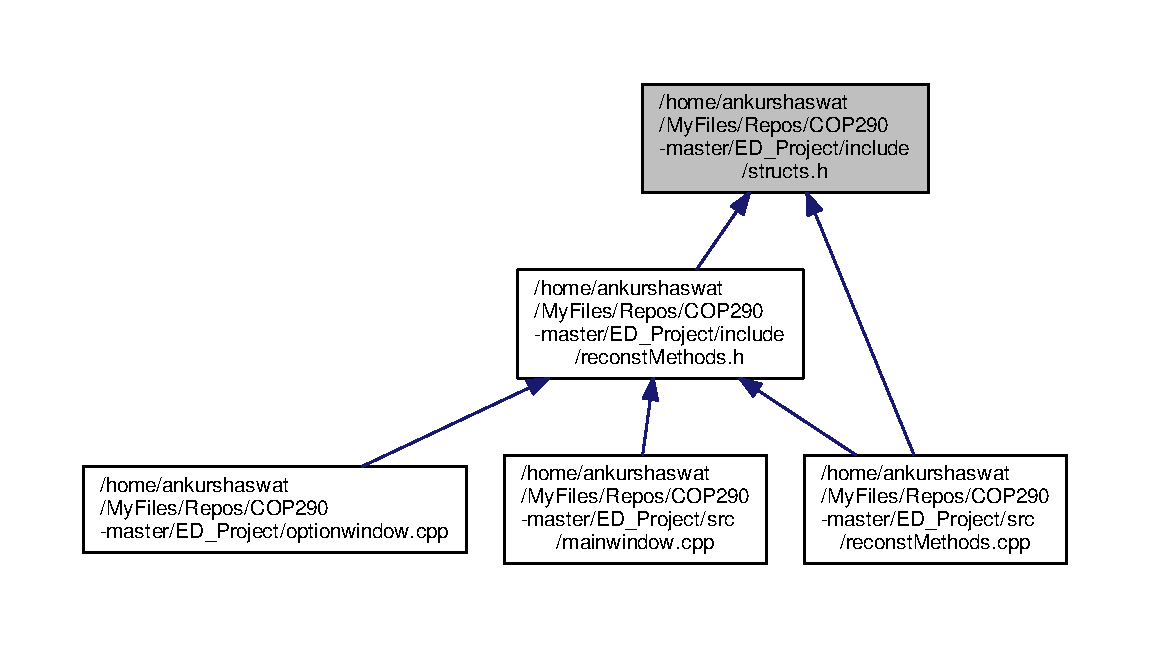
\includegraphics[width=350pt]{structs_8h__dep__incl}
\end{center}
\end{figure}
\subsection*{Classes}
\begin{DoxyCompactItemize}
\item 
class \hyperlink{classpartialOrder}{partial\+Order}
\end{DoxyCompactItemize}

\hypertarget{main_8cpp}{}\section{/home/ankurshaswat/\+My\+Files/\+Repos/\+C\+O\+P290-\/master/\+E\+D\+\_\+\+Project/main.cpp File Reference}
\label{main_8cpp}\index{/home/ankurshaswat/\+My\+Files/\+Repos/\+C\+O\+P290-\/master/\+E\+D\+\_\+\+Project/main.\+cpp@{/home/ankurshaswat/\+My\+Files/\+Repos/\+C\+O\+P290-\/master/\+E\+D\+\_\+\+Project/main.\+cpp}}
{\ttfamily \#include \char`\"{}mainwindow.\+h\char`\"{}}\newline
{\ttfamily \#include $<$Q\+Application$>$}\newline
{\ttfamily \#include \char`\"{}basic\+Components.\+h\char`\"{}}\newline
{\ttfamily \#include \char`\"{}obj\+Loader.\+h\char`\"{}}\newline
{\ttfamily \#include \char`\"{}optionwindow.\+h\char`\"{}}\newline
{\ttfamily \#include \char`\"{}hidden\+Lines.\+h\char`\"{}}\newline
{\ttfamily \#include \char`\"{}helperfunctions.\+h\char`\"{}}\newline
{\ttfamily \#include $<$stdio.\+h$>$}\newline
{\ttfamily \#include $<$iostream$>$}\newline
Include dependency graph for main.\+cpp\+:
\nopagebreak
\begin{figure}[H]
\begin{center}
\leavevmode
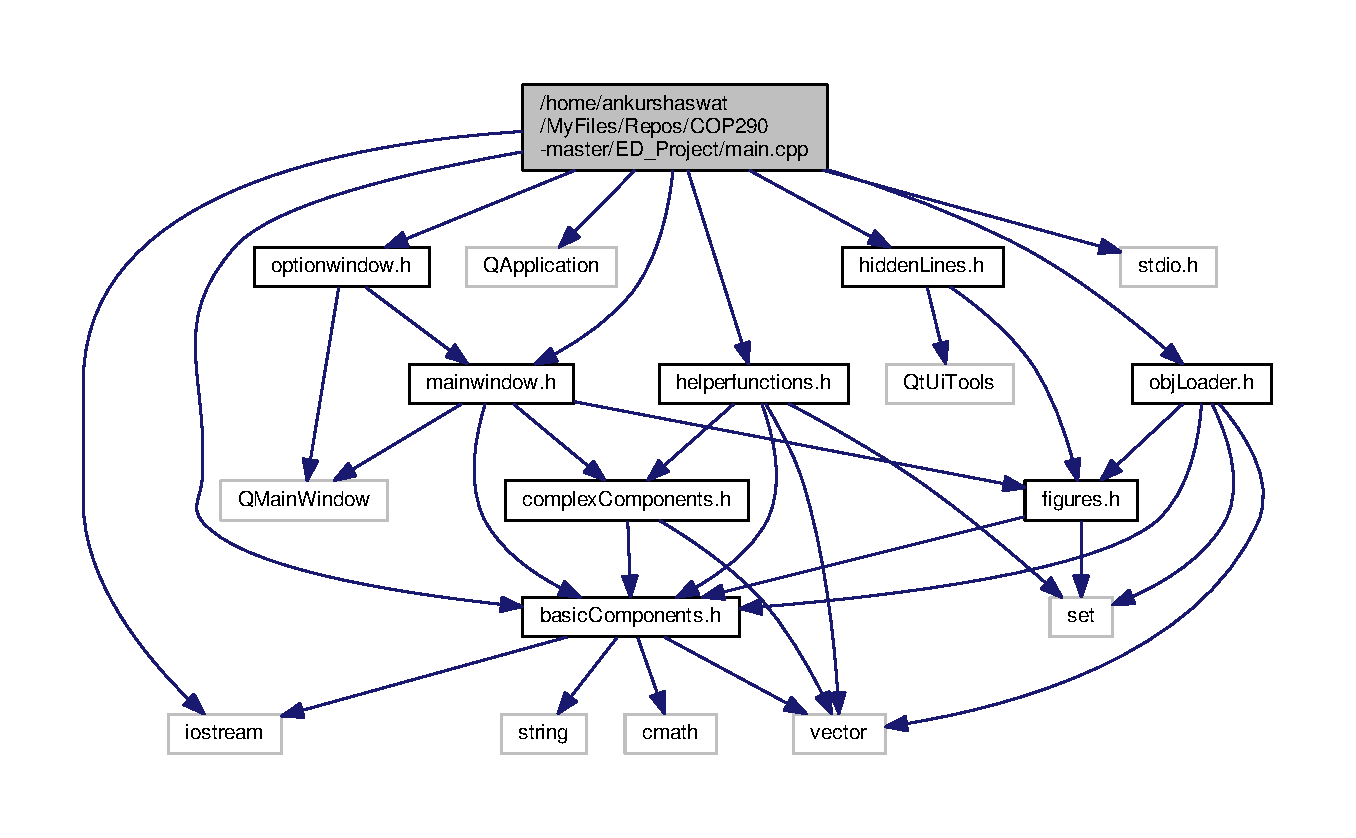
\includegraphics[width=350pt]{main_8cpp__incl}
\end{center}
\end{figure}
\subsection*{Functions}
\begin{DoxyCompactItemize}
\item 
int \hyperlink{main_8cpp_a0ddf1224851353fc92bfbff6f499fa97}{main} (int argc, char $\ast$argv\mbox{[}$\,$\mbox{]})
\end{DoxyCompactItemize}


\subsection{Function Documentation}
\mbox{\Hypertarget{main_8cpp_a0ddf1224851353fc92bfbff6f499fa97}\label{main_8cpp_a0ddf1224851353fc92bfbff6f499fa97}} 
\index{main.\+cpp@{main.\+cpp}!main@{main}}
\index{main@{main}!main.\+cpp@{main.\+cpp}}
\subsubsection{\texorpdfstring{main()}{main()}}
{\footnotesize\ttfamily int main (\begin{DoxyParamCaption}\item[{int}]{argc,  }\item[{char $\ast$}]{argv\mbox{[}$\,$\mbox{]} }\end{DoxyParamCaption})}


\hypertarget{optionwindow_8cpp}{}\section{/home/ankurshaswat/\+My\+Files/\+Repos/\+C\+O\+P290-\/master/\+E\+D\+\_\+\+Project/optionwindow.cpp File Reference}
\label{optionwindow_8cpp}\index{/home/ankurshaswat/\+My\+Files/\+Repos/\+C\+O\+P290-\/master/\+E\+D\+\_\+\+Project/optionwindow.\+cpp@{/home/ankurshaswat/\+My\+Files/\+Repos/\+C\+O\+P290-\/master/\+E\+D\+\_\+\+Project/optionwindow.\+cpp}}
{\ttfamily \#include \char`\"{}optionwindow.\+h\char`\"{}}\newline
{\ttfamily \#include \char`\"{}ui\+\_\+optionwindow.\+h\char`\"{}}\newline
{\ttfamily \#include $<$Q\+File\+Dialog$>$}\newline
{\ttfamily \#include $<$Q\+Message\+Box$>$}\newline
{\ttfamily \#include \char`\"{}mainwindow.\+h\char`\"{}}\newline
{\ttfamily \#include \char`\"{}obj\+Loader.\+h\char`\"{}}\newline
{\ttfamily \#include \char`\"{}reconst\+Methods.\+h\char`\"{}}\newline
{\ttfamily \#include \char`\"{}helperfunctions.\+h\char`\"{}}\newline
Include dependency graph for optionwindow.\+cpp\+:
\nopagebreak
\begin{figure}[H]
\begin{center}
\leavevmode
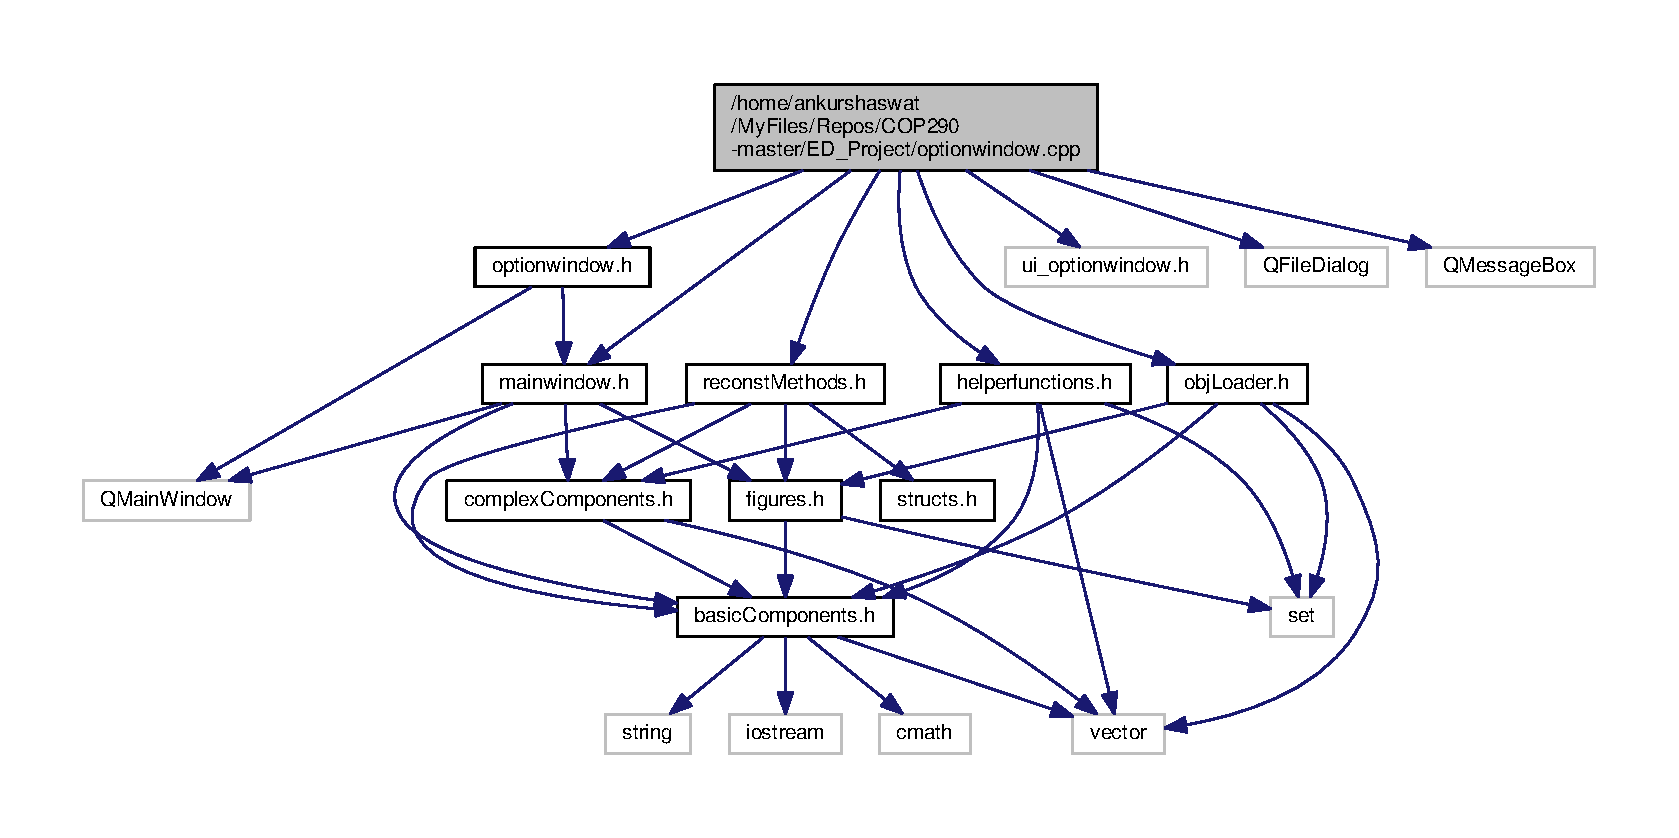
\includegraphics[width=350pt]{optionwindow_8cpp__incl}
\end{center}
\end{figure}

\hypertarget{optionwindow_8h}{}\section{/home/ankurshaswat/\+My\+Files/\+Repos/\+C\+O\+P290/working\+\_\+3d\+\_\+to\+\_\+2d/optionwindow.h File Reference}
\label{optionwindow_8h}\index{/home/ankurshaswat/\+My\+Files/\+Repos/\+C\+O\+P290/working\+\_\+3d\+\_\+to\+\_\+2d/optionwindow.\+h@{/home/ankurshaswat/\+My\+Files/\+Repos/\+C\+O\+P290/working\+\_\+3d\+\_\+to\+\_\+2d/optionwindow.\+h}}
{\ttfamily \#include \char`\"{}mainwindow.\+h\char`\"{}}\newline
{\ttfamily \#include $<$Q\+Main\+Window$>$}\newline
Include dependency graph for optionwindow.\+h\+:
\nopagebreak
\begin{figure}[H]
\begin{center}
\leavevmode
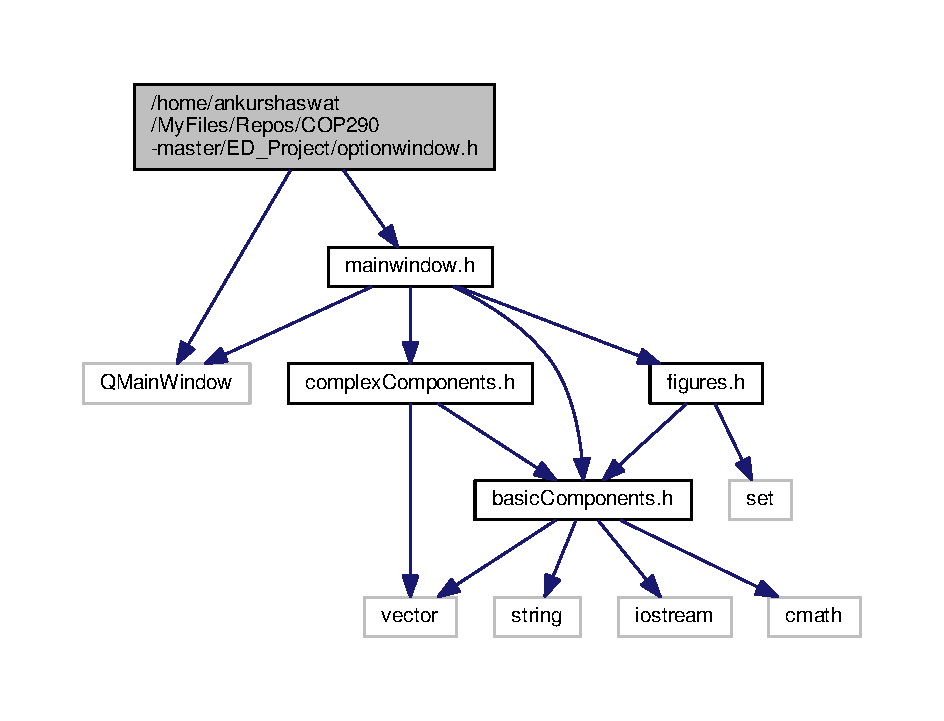
\includegraphics[width=350pt]{optionwindow_8h__incl}
\end{center}
\end{figure}
This graph shows which files directly or indirectly include this file\+:
\nopagebreak
\begin{figure}[H]
\begin{center}
\leavevmode
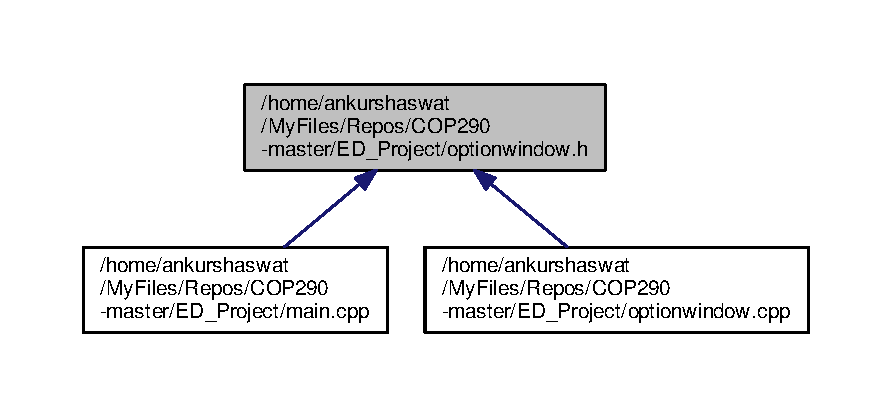
\includegraphics[width=350pt]{optionwindow_8h__dep__incl}
\end{center}
\end{figure}
\subsection*{Classes}
\begin{DoxyCompactItemize}
\item 
class \hyperlink{classoptionWindow}{option\+Window}
\end{DoxyCompactItemize}
\subsection*{Namespaces}
\begin{DoxyCompactItemize}
\item 
 \hyperlink{namespaceUi}{Ui}
\end{DoxyCompactItemize}

\hypertarget{complexcomponents_8cpp}{}\section{/home/ankurshaswat/\+My\+Files/\+Repos/\+C\+O\+P290/working\+\_\+3d\+\_\+to\+\_\+2d/src/complexcomponents.cpp File Reference}
\label{complexcomponents_8cpp}\index{/home/ankurshaswat/\+My\+Files/\+Repos/\+C\+O\+P290/working\+\_\+3d\+\_\+to\+\_\+2d/src/complexcomponents.\+cpp@{/home/ankurshaswat/\+My\+Files/\+Repos/\+C\+O\+P290/working\+\_\+3d\+\_\+to\+\_\+2d/src/complexcomponents.\+cpp}}
{\ttfamily \#include \char`\"{}complex\+Components.\+h\char`\"{}}\newline
{\ttfamily \#include \char`\"{}helperfunctions.\+h\char`\"{}}\newline
Include dependency graph for complexcomponents.\+cpp\+:
\nopagebreak
\begin{figure}[H]
\begin{center}
\leavevmode
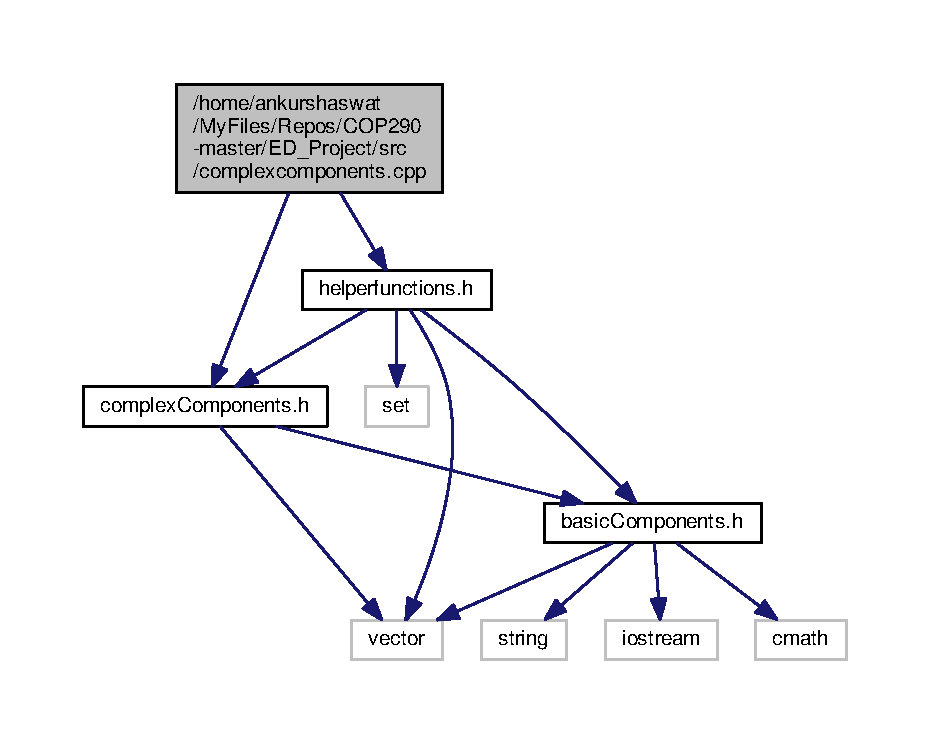
\includegraphics[width=350pt]{complexcomponents_8cpp__incl}
\end{center}
\end{figure}
\subsection*{Macros}
\begin{DoxyCompactItemize}
\item 
\#define \hyperlink{complexcomponents_8cpp_a598a3330b3c21701223ee0ca14316eca}{PI}~3.\+14159265
\end{DoxyCompactItemize}


\subsection{Macro Definition Documentation}
\mbox{\Hypertarget{complexcomponents_8cpp_a598a3330b3c21701223ee0ca14316eca}\label{complexcomponents_8cpp_a598a3330b3c21701223ee0ca14316eca}} 
\index{complexcomponents.\+cpp@{complexcomponents.\+cpp}!PI@{PI}}
\index{PI@{PI}!complexcomponents.\+cpp@{complexcomponents.\+cpp}}
\subsubsection{\texorpdfstring{PI}{PI}}
{\footnotesize\ttfamily \#define PI~3.\+14159265}


\hypertarget{figures_8cpp}{}\section{/home/ankurshaswat/\+My\+Files/\+Repos/\+C\+O\+P290/working\+\_\+3d\+\_\+to\+\_\+2d/src/figures.cpp File Reference}
\label{figures_8cpp}\index{/home/ankurshaswat/\+My\+Files/\+Repos/\+C\+O\+P290/working\+\_\+3d\+\_\+to\+\_\+2d/src/figures.\+cpp@{/home/ankurshaswat/\+My\+Files/\+Repos/\+C\+O\+P290/working\+\_\+3d\+\_\+to\+\_\+2d/src/figures.\+cpp}}
{\ttfamily \#include \char`\"{}figures.\+h\char`\"{}}\newline
{\ttfamily \#include $<$math.\+h$>$}\newline
{\ttfamily \#include $<$set$>$}\newline
{\ttfamily \#include \char`\"{}basic\+Components.\+h\char`\"{}}\newline
{\ttfamily \#include $<$vector$>$}\newline
{\ttfamily \#include \char`\"{}obj\+Loader.\+h\char`\"{}}\newline
{\ttfamily \#include \char`\"{}stdio.\+h\char`\"{}}\newline
{\ttfamily \#include \char`\"{}helperfunctions.\+h\char`\"{}}\newline
Include dependency graph for figures.\+cpp\+:
\nopagebreak
\begin{figure}[H]
\begin{center}
\leavevmode
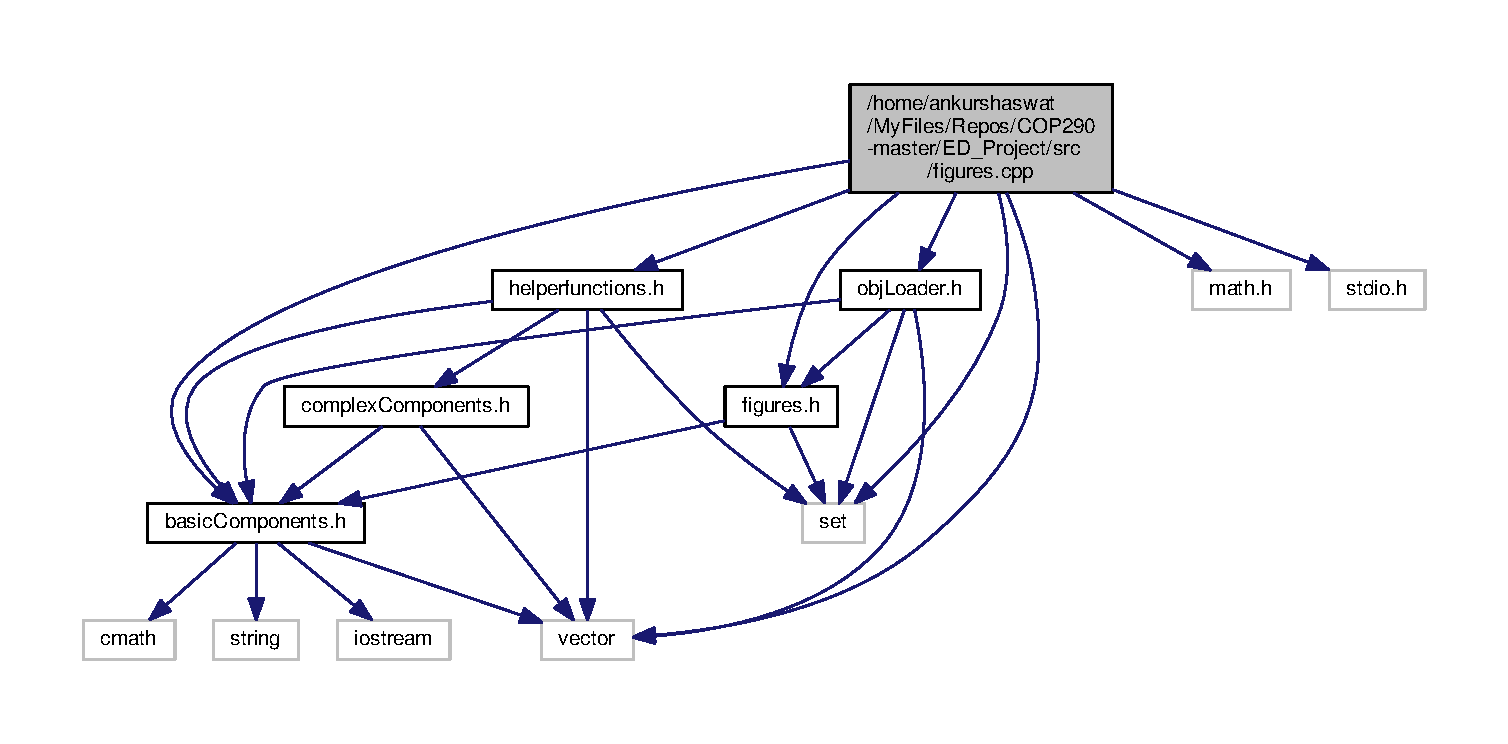
\includegraphics[width=350pt]{figures_8cpp__incl}
\end{center}
\end{figure}

\hypertarget{helperfunctions_8cpp}{}\section{/home/ankurshaswat/\+My\+Files/\+Repos/\+C\+O\+P290-\/master/\+E\+D\+\_\+\+Project/src/helperfunctions.cpp File Reference}
\label{helperfunctions_8cpp}\index{/home/ankurshaswat/\+My\+Files/\+Repos/\+C\+O\+P290-\/master/\+E\+D\+\_\+\+Project/src/helperfunctions.\+cpp@{/home/ankurshaswat/\+My\+Files/\+Repos/\+C\+O\+P290-\/master/\+E\+D\+\_\+\+Project/src/helperfunctions.\+cpp}}
{\ttfamily \#include \char`\"{}helperfunctions.\+h\char`\"{}}\newline
{\ttfamily \#include \char`\"{}basic\+Components.\+h\char`\"{}}\newline
{\ttfamily \#include \char`\"{}complex\+Components.\+h\char`\"{}}\newline
{\ttfamily \#include \char`\"{}math.\+h\char`\"{}}\newline
{\ttfamily \#include $<$vector$>$}\newline
{\ttfamily \#include $<$algorithm$>$}\newline
{\ttfamily \#include $<$set$>$}\newline
Include dependency graph for helperfunctions.\+cpp\+:
\nopagebreak
\begin{figure}[H]
\begin{center}
\leavevmode
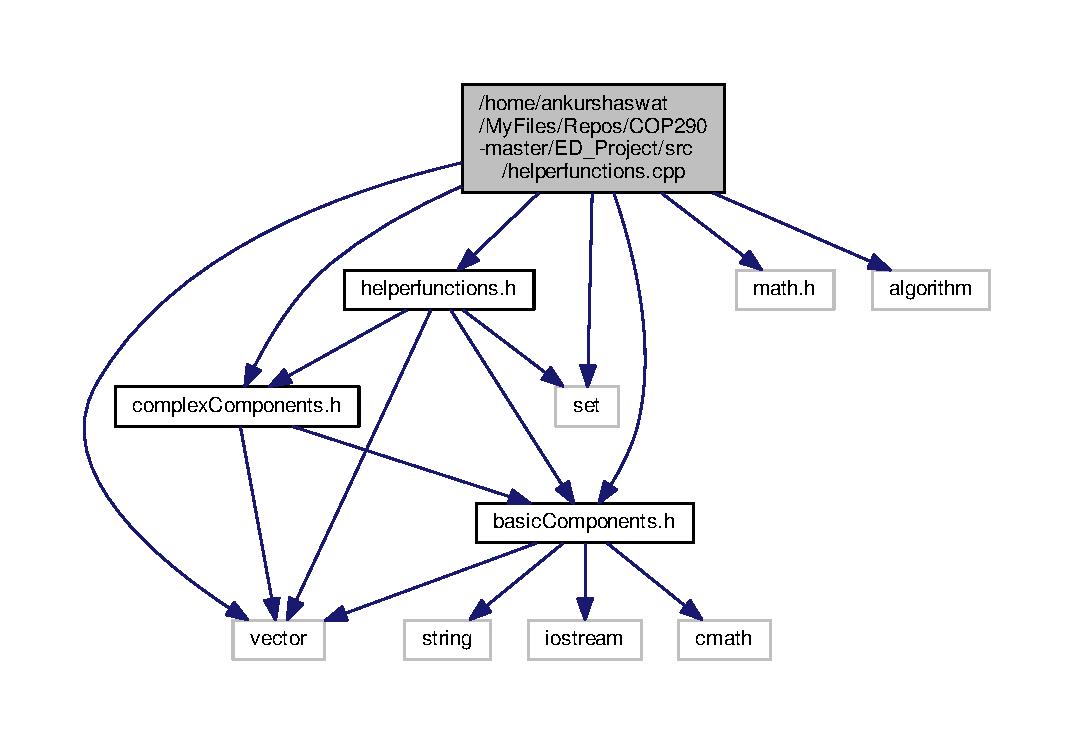
\includegraphics[width=350pt]{helperfunctions_8cpp__incl}
\end{center}
\end{figure}
\subsection*{Macros}
\begin{DoxyCompactItemize}
\item 
\#define \hyperlink{helperfunctions_8cpp_a598a3330b3c21701223ee0ca14316eca}{PI}~3.\+14159265
\item 
\#define \hyperlink{helperfunctions_8cpp_a12c2040f25d8e3a7b9e1c2024c618cb6}{I\+NF}~1000000
\item 
\#define \hyperlink{helperfunctions_8cpp_a06b50f1ca7258a9862c39d3ed354bf7c}{epsilon}~0.\+1
\end{DoxyCompactItemize}
\subsection*{Functions}
\begin{DoxyCompactItemize}
\item 
\hyperlink{structVertice}{Vertice} \hyperlink{helperfunctions_8cpp_a4a9bde2a0de0b0199de919d3b4628e89}{transform} (\hyperlink{structVertice}{Vertice} v\+\_\+in, double Xrot, double Yrot, double Zrot, double Xoff, double Yoff, double Zoff)
\begin{DoxyCompactList}\small\item\em Transforms a vertice (rotation and offset) using matrix multiplication and returns a new \hyperlink{structVertice}{Vertice} object. \end{DoxyCompactList}\item 
pair$<$ int, \hyperlink{structVertice}{Vertice} $>$ \hyperlink{helperfunctions_8cpp_aeeffe6b314e92051412034d7e06b03d6}{get\+\_\+intersection} (\hyperlink{structEdge}{Edge} a, \hyperlink{structEdge}{Edge} b)
\begin{DoxyCompactList}\small\item\em Finds intersection of two edges (line segments) and also returns error if intersection does not exist. \end{DoxyCompactList}\item 
bool \hyperlink{helperfunctions_8cpp_a948ecdee044f4ebf6f132257557292fc}{is\+\_\+inside} (\hyperlink{structVertice}{Vertice} v, set$<$ \hyperlink{structEdge}{Edge} $>$ edge\+Set)
\begin{DoxyCompactList}\small\item\em Checks whether a vertice is inside (in 2d) of a face formed by an edge loop. \end{DoxyCompactList}\item 
bool \hyperlink{helperfunctions_8cpp_ab52930079ad22c64677a4bcafd8728c7}{is\+Subset} (vector$<$ int $>$ \&a, vector$<$ int $>$ \&b)
\item 
int \hyperlink{helperfunctions_8cpp_aaa98082eb9298793e9b30843abb80b6a}{vertice\+Present} (vector$<$ \hyperlink{structVertice}{Vertice} $>$ \&a, \hyperlink{structVertice}{Vertice} b)
\begin{DoxyCompactList}\small\item\em Checks if a vertice is present in a vector of vertices. \end{DoxyCompactList}\item 
\hyperlink{classWireFrame}{Wire\+Frame} \hyperlink{helperfunctions_8cpp_a9bcea272ffd067ba2d045be1af40cedf}{modify\+Wireframe} (\hyperlink{classWireFrame}{Wire\+Frame} wf, \hyperlink{structVertice}{Vertice} v)
\begin{DoxyCompactList}\small\item\em Takes a wireframe and subtracts coordinates of v from all its edge vertices. \end{DoxyCompactList}\end{DoxyCompactItemize}


\subsection{Macro Definition Documentation}
\mbox{\Hypertarget{helperfunctions_8cpp_a06b50f1ca7258a9862c39d3ed354bf7c}\label{helperfunctions_8cpp_a06b50f1ca7258a9862c39d3ed354bf7c}} 
\index{helperfunctions.\+cpp@{helperfunctions.\+cpp}!epsilon@{epsilon}}
\index{epsilon@{epsilon}!helperfunctions.\+cpp@{helperfunctions.\+cpp}}
\subsubsection{\texorpdfstring{epsilon}{epsilon}}
{\footnotesize\ttfamily \#define epsilon~0.\+1}

\mbox{\Hypertarget{helperfunctions_8cpp_a12c2040f25d8e3a7b9e1c2024c618cb6}\label{helperfunctions_8cpp_a12c2040f25d8e3a7b9e1c2024c618cb6}} 
\index{helperfunctions.\+cpp@{helperfunctions.\+cpp}!I\+NF@{I\+NF}}
\index{I\+NF@{I\+NF}!helperfunctions.\+cpp@{helperfunctions.\+cpp}}
\subsubsection{\texorpdfstring{I\+NF}{INF}}
{\footnotesize\ttfamily \#define I\+NF~1000000}

\mbox{\Hypertarget{helperfunctions_8cpp_a598a3330b3c21701223ee0ca14316eca}\label{helperfunctions_8cpp_a598a3330b3c21701223ee0ca14316eca}} 
\index{helperfunctions.\+cpp@{helperfunctions.\+cpp}!PI@{PI}}
\index{PI@{PI}!helperfunctions.\+cpp@{helperfunctions.\+cpp}}
\subsubsection{\texorpdfstring{PI}{PI}}
{\footnotesize\ttfamily \#define PI~3.\+14159265}



\subsection{Function Documentation}
\mbox{\Hypertarget{helperfunctions_8cpp_aeeffe6b314e92051412034d7e06b03d6}\label{helperfunctions_8cpp_aeeffe6b314e92051412034d7e06b03d6}} 
\index{helperfunctions.\+cpp@{helperfunctions.\+cpp}!get\+\_\+intersection@{get\+\_\+intersection}}
\index{get\+\_\+intersection@{get\+\_\+intersection}!helperfunctions.\+cpp@{helperfunctions.\+cpp}}
\subsubsection{\texorpdfstring{get\+\_\+intersection()}{get\_intersection()}}
{\footnotesize\ttfamily pair$<$int,\hyperlink{structVertice}{Vertice}$>$ get\+\_\+intersection (\begin{DoxyParamCaption}\item[{\hyperlink{structEdge}{Edge}}]{a,  }\item[{\hyperlink{structEdge}{Edge}}]{b }\end{DoxyParamCaption})}



Finds intersection of two edges (line segments) and also returns error if intersection does not exist. 

returns (1,point of intersection) if intersecting, (0,\+\_\+) if overlapping and (-\/1,\+\_\+) if parallel Both edges are 2D edges \mbox{\Hypertarget{helperfunctions_8cpp_a948ecdee044f4ebf6f132257557292fc}\label{helperfunctions_8cpp_a948ecdee044f4ebf6f132257557292fc}} 
\index{helperfunctions.\+cpp@{helperfunctions.\+cpp}!is\+\_\+inside@{is\+\_\+inside}}
\index{is\+\_\+inside@{is\+\_\+inside}!helperfunctions.\+cpp@{helperfunctions.\+cpp}}
\subsubsection{\texorpdfstring{is\+\_\+inside()}{is\_inside()}}
{\footnotesize\ttfamily bool is\+\_\+inside (\begin{DoxyParamCaption}\item[{\hyperlink{structVertice}{Vertice}}]{v,  }\item[{set$<$ \hyperlink{structEdge}{Edge} $>$}]{edge\+Set }\end{DoxyParamCaption})}



Checks whether a vertice is inside (in 2d) of a face formed by an edge loop. 

Checks if vertex is inside the polygon defined by the edge set \mbox{\Hypertarget{helperfunctions_8cpp_ab52930079ad22c64677a4bcafd8728c7}\label{helperfunctions_8cpp_ab52930079ad22c64677a4bcafd8728c7}} 
\index{helperfunctions.\+cpp@{helperfunctions.\+cpp}!is\+Subset@{is\+Subset}}
\index{is\+Subset@{is\+Subset}!helperfunctions.\+cpp@{helperfunctions.\+cpp}}
\subsubsection{\texorpdfstring{is\+Subset()}{isSubset()}}
{\footnotesize\ttfamily bool is\+Subset (\begin{DoxyParamCaption}\item[{vector$<$ int $>$ \&}]{a,  }\item[{vector$<$ int $>$ \&}]{b }\end{DoxyParamCaption})}

A simple helper function to check if a is a subset of b \mbox{\Hypertarget{helperfunctions_8cpp_a9bcea272ffd067ba2d045be1af40cedf}\label{helperfunctions_8cpp_a9bcea272ffd067ba2d045be1af40cedf}} 
\index{helperfunctions.\+cpp@{helperfunctions.\+cpp}!modify\+Wireframe@{modify\+Wireframe}}
\index{modify\+Wireframe@{modify\+Wireframe}!helperfunctions.\+cpp@{helperfunctions.\+cpp}}
\subsubsection{\texorpdfstring{modify\+Wireframe()}{modifyWireframe()}}
{\footnotesize\ttfamily \hyperlink{classWireFrame}{Wire\+Frame} modify\+Wireframe (\begin{DoxyParamCaption}\item[{\hyperlink{classWireFrame}{Wire\+Frame}}]{wf,  }\item[{\hyperlink{structVertice}{Vertice}}]{v }\end{DoxyParamCaption})}



Takes a wireframe and subtracts coordinates of v from all its edge vertices. 

\mbox{\Hypertarget{helperfunctions_8cpp_a4a9bde2a0de0b0199de919d3b4628e89}\label{helperfunctions_8cpp_a4a9bde2a0de0b0199de919d3b4628e89}} 
\index{helperfunctions.\+cpp@{helperfunctions.\+cpp}!transform@{transform}}
\index{transform@{transform}!helperfunctions.\+cpp@{helperfunctions.\+cpp}}
\subsubsection{\texorpdfstring{transform()}{transform()}}
{\footnotesize\ttfamily \hyperlink{structVertice}{Vertice} transform (\begin{DoxyParamCaption}\item[{\hyperlink{structVertice}{Vertice}}]{v\+\_\+in,  }\item[{double}]{Xrot,  }\item[{double}]{Yrot,  }\item[{double}]{Zrot,  }\item[{double}]{Xoff,  }\item[{double}]{Yoff,  }\item[{double}]{Zoff }\end{DoxyParamCaption})}



Transforms a vertice (rotation and offset) using matrix multiplication and returns a new \hyperlink{structVertice}{Vertice} object. 

get transformed 3D object \mbox{\Hypertarget{helperfunctions_8cpp_aaa98082eb9298793e9b30843abb80b6a}\label{helperfunctions_8cpp_aaa98082eb9298793e9b30843abb80b6a}} 
\index{helperfunctions.\+cpp@{helperfunctions.\+cpp}!vertice\+Present@{vertice\+Present}}
\index{vertice\+Present@{vertice\+Present}!helperfunctions.\+cpp@{helperfunctions.\+cpp}}
\subsubsection{\texorpdfstring{vertice\+Present()}{verticePresent()}}
{\footnotesize\ttfamily int vertice\+Present (\begin{DoxyParamCaption}\item[{vector$<$ \hyperlink{structVertice}{Vertice} $>$ \&}]{a,  }\item[{\hyperlink{structVertice}{Vertice}}]{b }\end{DoxyParamCaption})}



Checks if a vertice is present in a vector of vertices. 

A simple helper function which checks if vertex is already present in vector (allowing for some error correction) 
\hypertarget{hiddenLines_8cpp}{}\section{/home/ankurshaswat/\+My\+Files/\+Repos/\+C\+O\+P290/working\+\_\+3d\+\_\+to\+\_\+2d/src/hidden\+Lines.cpp File Reference}
\label{hiddenLines_8cpp}\index{/home/ankurshaswat/\+My\+Files/\+Repos/\+C\+O\+P290/working\+\_\+3d\+\_\+to\+\_\+2d/src/hidden\+Lines.\+cpp@{/home/ankurshaswat/\+My\+Files/\+Repos/\+C\+O\+P290/working\+\_\+3d\+\_\+to\+\_\+2d/src/hidden\+Lines.\+cpp}}
{\ttfamily \#include \char`\"{}basic\+Components.\+h\char`\"{}}\newline
{\ttfamily \#include \char`\"{}obj\+Loader.\+h\char`\"{}}\newline
{\ttfamily \#include \char`\"{}figures.\+h\char`\"{}}\newline
{\ttfamily \#include \char`\"{}hidden\+Lines.\+h\char`\"{}}\newline
{\ttfamily \#include \char`\"{}helperfunctions.\+h\char`\"{}}\newline
{\ttfamily \#include $<$stdio.\+h$>$}\newline
{\ttfamily \#include $<$Qt\+Ui\+Tools$>$}\newline
{\ttfamily \#include $<$iostream$>$}\newline
{\ttfamily \#include $<$vector$>$}\newline
{\ttfamily \#include $<$set$>$}\newline
{\ttfamily \#include $<$cmath$>$}\newline
Include dependency graph for hidden\+Lines.\+cpp\+:
\nopagebreak
\begin{figure}[H]
\begin{center}
\leavevmode
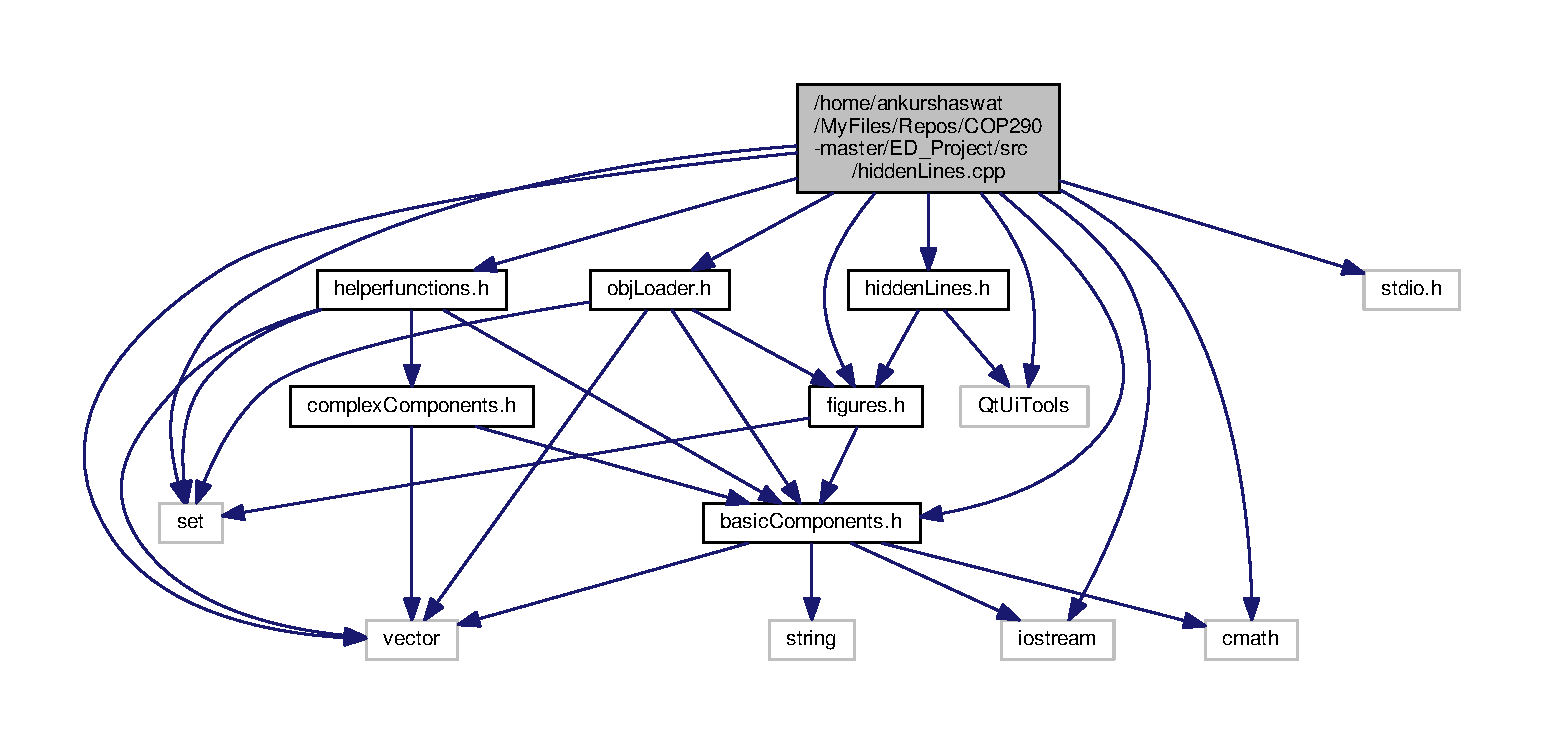
\includegraphics[width=350pt]{hiddenLines_8cpp__incl}
\end{center}
\end{figure}
\subsection*{Macros}
\begin{DoxyCompactItemize}
\item 
\#define \hyperlink{hiddenLines_8cpp_a12c2040f25d8e3a7b9e1c2024c618cb6}{I\+NF}~1000000
\item 
\#define \hyperlink{hiddenLines_8cpp_a06b50f1ca7258a9862c39d3ed354bf7c}{epsilon}~0.\+1
\end{DoxyCompactItemize}
\subsection*{Functions}
\begin{DoxyCompactItemize}
\item 
bool \hyperlink{hiddenLines_8cpp_a836768e232c104dd933ab255f798d0d5}{opposite\+\_\+side} (vector$<$ \hyperlink{structVertice}{Vertice} $>$ \&face\+Vertices, \hyperlink{structVertice}{Vertice} e, \hyperlink{structVertice}{Vertice} f)
\item 
\hyperlink{structVertice}{Vertice} \hyperlink{hiddenLines_8cpp_a5245c9f2d3321def89057b7d397d84e3}{back\+\_\+proj} (\hyperlink{structVertice}{Vertice} v, \hyperlink{structEdge}{Edge} e, int plane)
\item 
\hyperlink{structVertice}{Vertice} \hyperlink{hiddenLines_8cpp_aba67ff1d3d9b1af057a7743947d8a716}{get\+\_\+vertex\+\_\+inf} (\hyperlink{structVertice}{Vertice} x, int plane)
\item 
void \hyperlink{hiddenLines_8cpp_aafdedb0fe0862c4196f86c1c1828d27f}{render2\+D\+Hidden} (\hyperlink{classFig3D}{Fig3D} \&object3D, Q\+Painter \&painter, int plane)
\begin{DoxyCompactList}\small\item\em Renders the figure and also marks lines as hidden where they are hidden by some plane. \end{DoxyCompactList}\end{DoxyCompactItemize}


\subsection{Macro Definition Documentation}
\mbox{\Hypertarget{hiddenLines_8cpp_a06b50f1ca7258a9862c39d3ed354bf7c}\label{hiddenLines_8cpp_a06b50f1ca7258a9862c39d3ed354bf7c}} 
\index{hidden\+Lines.\+cpp@{hidden\+Lines.\+cpp}!epsilon@{epsilon}}
\index{epsilon@{epsilon}!hidden\+Lines.\+cpp@{hidden\+Lines.\+cpp}}
\subsubsection{\texorpdfstring{epsilon}{epsilon}}
{\footnotesize\ttfamily \#define epsilon~0.\+1}

\mbox{\Hypertarget{hiddenLines_8cpp_a12c2040f25d8e3a7b9e1c2024c618cb6}\label{hiddenLines_8cpp_a12c2040f25d8e3a7b9e1c2024c618cb6}} 
\index{hidden\+Lines.\+cpp@{hidden\+Lines.\+cpp}!I\+NF@{I\+NF}}
\index{I\+NF@{I\+NF}!hidden\+Lines.\+cpp@{hidden\+Lines.\+cpp}}
\subsubsection{\texorpdfstring{I\+NF}{INF}}
{\footnotesize\ttfamily \#define I\+NF~1000000}



\subsection{Function Documentation}
\mbox{\Hypertarget{hiddenLines_8cpp_a5245c9f2d3321def89057b7d397d84e3}\label{hiddenLines_8cpp_a5245c9f2d3321def89057b7d397d84e3}} 
\index{hidden\+Lines.\+cpp@{hidden\+Lines.\+cpp}!back\+\_\+proj@{back\+\_\+proj}}
\index{back\+\_\+proj@{back\+\_\+proj}!hidden\+Lines.\+cpp@{hidden\+Lines.\+cpp}}
\subsubsection{\texorpdfstring{back\+\_\+proj()}{back\_proj()}}
{\footnotesize\ttfamily \hyperlink{structVertice}{Vertice} back\+\_\+proj (\begin{DoxyParamCaption}\item[{\hyperlink{structVertice}{Vertice}}]{v,  }\item[{\hyperlink{structEdge}{Edge}}]{e,  }\item[{int}]{plane }\end{DoxyParamCaption})}

returns 3D vertex on \hyperlink{structEdge}{Edge} e whose projection is v \mbox{\Hypertarget{hiddenLines_8cpp_aba67ff1d3d9b1af057a7743947d8a716}\label{hiddenLines_8cpp_aba67ff1d3d9b1af057a7743947d8a716}} 
\index{hidden\+Lines.\+cpp@{hidden\+Lines.\+cpp}!get\+\_\+vertex\+\_\+inf@{get\+\_\+vertex\+\_\+inf}}
\index{get\+\_\+vertex\+\_\+inf@{get\+\_\+vertex\+\_\+inf}!hidden\+Lines.\+cpp@{hidden\+Lines.\+cpp}}
\subsubsection{\texorpdfstring{get\+\_\+vertex\+\_\+inf()}{get\_vertex\_inf()}}
{\footnotesize\ttfamily \hyperlink{structVertice}{Vertice} get\+\_\+vertex\+\_\+inf (\begin{DoxyParamCaption}\item[{\hyperlink{structVertice}{Vertice}}]{x,  }\item[{int}]{plane }\end{DoxyParamCaption})}

Returns Vertex at infinity for the corresponding projection plane (to check if a vertex and our view point lie on opposite side of a face) \mbox{\Hypertarget{hiddenLines_8cpp_a836768e232c104dd933ab255f798d0d5}\label{hiddenLines_8cpp_a836768e232c104dd933ab255f798d0d5}} 
\index{hidden\+Lines.\+cpp@{hidden\+Lines.\+cpp}!opposite\+\_\+side@{opposite\+\_\+side}}
\index{opposite\+\_\+side@{opposite\+\_\+side}!hidden\+Lines.\+cpp@{hidden\+Lines.\+cpp}}
\subsubsection{\texorpdfstring{opposite\+\_\+side()}{opposite\_side()}}
{\footnotesize\ttfamily bool opposite\+\_\+side (\begin{DoxyParamCaption}\item[{vector$<$ \hyperlink{structVertice}{Vertice} $>$ \&}]{face\+Vertices,  }\item[{\hyperlink{structVertice}{Vertice}}]{e,  }\item[{\hyperlink{structVertice}{Vertice}}]{f }\end{DoxyParamCaption})}

returns true if a and b are on opposite side of plane formed by face\+Vertices , false otherwise \mbox{\Hypertarget{hiddenLines_8cpp_aafdedb0fe0862c4196f86c1c1828d27f}\label{hiddenLines_8cpp_aafdedb0fe0862c4196f86c1c1828d27f}} 
\index{hidden\+Lines.\+cpp@{hidden\+Lines.\+cpp}!render2\+D\+Hidden@{render2\+D\+Hidden}}
\index{render2\+D\+Hidden@{render2\+D\+Hidden}!hidden\+Lines.\+cpp@{hidden\+Lines.\+cpp}}
\subsubsection{\texorpdfstring{render2\+D\+Hidden()}{render2DHidden()}}
{\footnotesize\ttfamily void render2\+D\+Hidden (\begin{DoxyParamCaption}\item[{\hyperlink{classFig3D}{Fig3D} \&}]{object3D,  }\item[{Q\+Painter \&}]{painter,  }\item[{int}]{plane }\end{DoxyParamCaption})}



Renders the figure and also marks lines as hidden where they are hidden by some plane. 


\hypertarget{mainwindow_8cpp}{}\section{/home/ankurshaswat/\+My\+Files/\+Repos/\+C\+O\+P290/working\+\_\+3d\+\_\+to\+\_\+2d/src/mainwindow.cpp File Reference}
\label{mainwindow_8cpp}\index{/home/ankurshaswat/\+My\+Files/\+Repos/\+C\+O\+P290/working\+\_\+3d\+\_\+to\+\_\+2d/src/mainwindow.\+cpp@{/home/ankurshaswat/\+My\+Files/\+Repos/\+C\+O\+P290/working\+\_\+3d\+\_\+to\+\_\+2d/src/mainwindow.\+cpp}}
{\ttfamily \#include \char`\"{}mainwindow.\+h\char`\"{}}\newline
{\ttfamily \#include \char`\"{}ui\+\_\+mainwindow.\+h\char`\"{}}\newline
{\ttfamily \#include $<$string.\+h$>$}\newline
{\ttfamily \#include $<$set$>$}\newline
{\ttfamily \#include $<$Q\+Gui\+Application$>$}\newline
{\ttfamily \#include $<$Qt\+Ui\+Tools$>$}\newline
{\ttfamily \#include \char`\"{}obj\+Loader.\+h\char`\"{}}\newline
{\ttfamily \#include \char`\"{}figures.\+h\char`\"{}}\newline
{\ttfamily \#include \char`\"{}complex\+Components.\+h\char`\"{}}\newline
{\ttfamily \#include \char`\"{}render\+Methods.\+h\char`\"{}}\newline
{\ttfamily \#include \char`\"{}hidden\+Lines.\+h\char`\"{}}\newline
{\ttfamily \#include \char`\"{}reconst\+Methods.\+h\char`\"{}}\newline
Include dependency graph for mainwindow.\+cpp\+:
\nopagebreak
\begin{figure}[H]
\begin{center}
\leavevmode
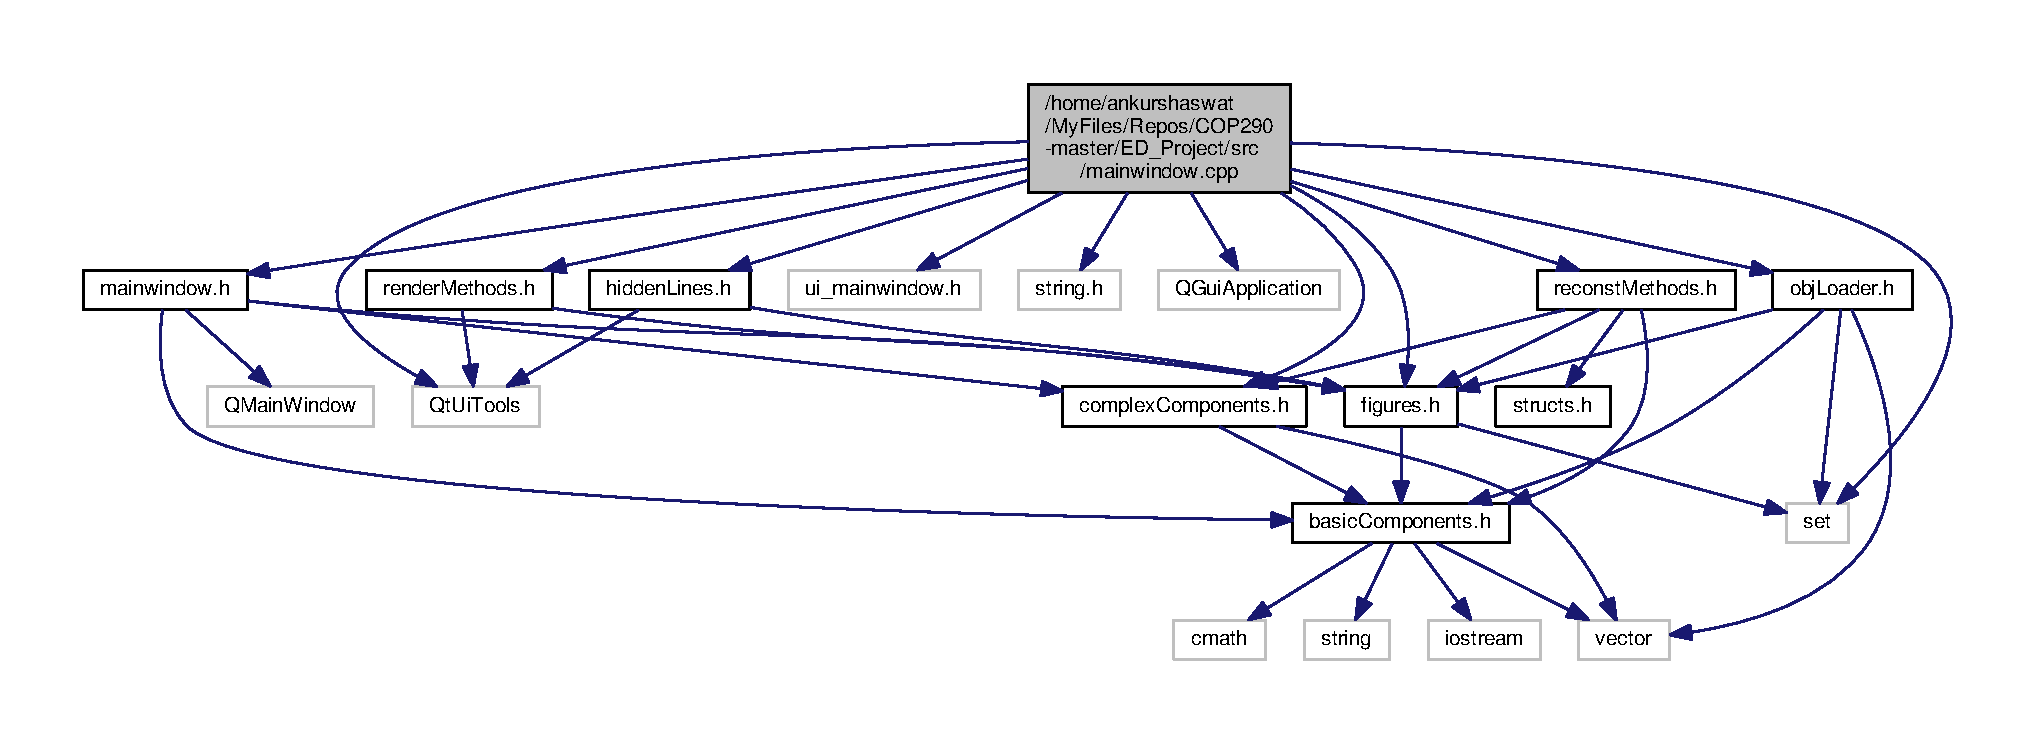
\includegraphics[width=350pt]{mainwindow_8cpp__incl}
\end{center}
\end{figure}
\subsection*{Functions}
\begin{DoxyCompactItemize}
\item 
void \hyperlink{mainwindow_8cpp_a5a937b34175a44a69ba8476407f8131b}{q\+Normalize\+Angle} (int \&angle)
\end{DoxyCompactItemize}


\subsection{Function Documentation}
\mbox{\Hypertarget{mainwindow_8cpp_a5a937b34175a44a69ba8476407f8131b}\label{mainwindow_8cpp_a5a937b34175a44a69ba8476407f8131b}} 
\index{mainwindow.\+cpp@{mainwindow.\+cpp}!q\+Normalize\+Angle@{q\+Normalize\+Angle}}
\index{q\+Normalize\+Angle@{q\+Normalize\+Angle}!mainwindow.\+cpp@{mainwindow.\+cpp}}
\subsubsection{\texorpdfstring{q\+Normalize\+Angle()}{qNormalizeAngle()}}
{\footnotesize\ttfamily void q\+Normalize\+Angle (\begin{DoxyParamCaption}\item[{int \&}]{angle }\end{DoxyParamCaption})}


\hypertarget{objLoader_8cpp}{}\section{/home/ankurshaswat/\+My\+Files/\+Repos/\+C\+O\+P290/working\+\_\+3d\+\_\+to\+\_\+2d/src/obj\+Loader.cpp File Reference}
\label{objLoader_8cpp}\index{/home/ankurshaswat/\+My\+Files/\+Repos/\+C\+O\+P290/working\+\_\+3d\+\_\+to\+\_\+2d/src/obj\+Loader.\+cpp@{/home/ankurshaswat/\+My\+Files/\+Repos/\+C\+O\+P290/working\+\_\+3d\+\_\+to\+\_\+2d/src/obj\+Loader.\+cpp}}
{\ttfamily \#include \char`\"{}obj\+Loader.\+h\char`\"{}}\newline
{\ttfamily \#include \char`\"{}figures.\+h\char`\"{}}\newline
{\ttfamily \#include $<$set$>$}\newline
{\ttfamily \#include $<$vector$>$}\newline
{\ttfamily \#include $<$iterator$>$}\newline
{\ttfamily \#include $<$cstring$>$}\newline
{\ttfamily \#include $<$iostream$>$}\newline
Include dependency graph for obj\+Loader.\+cpp\+:
\nopagebreak
\begin{figure}[H]
\begin{center}
\leavevmode
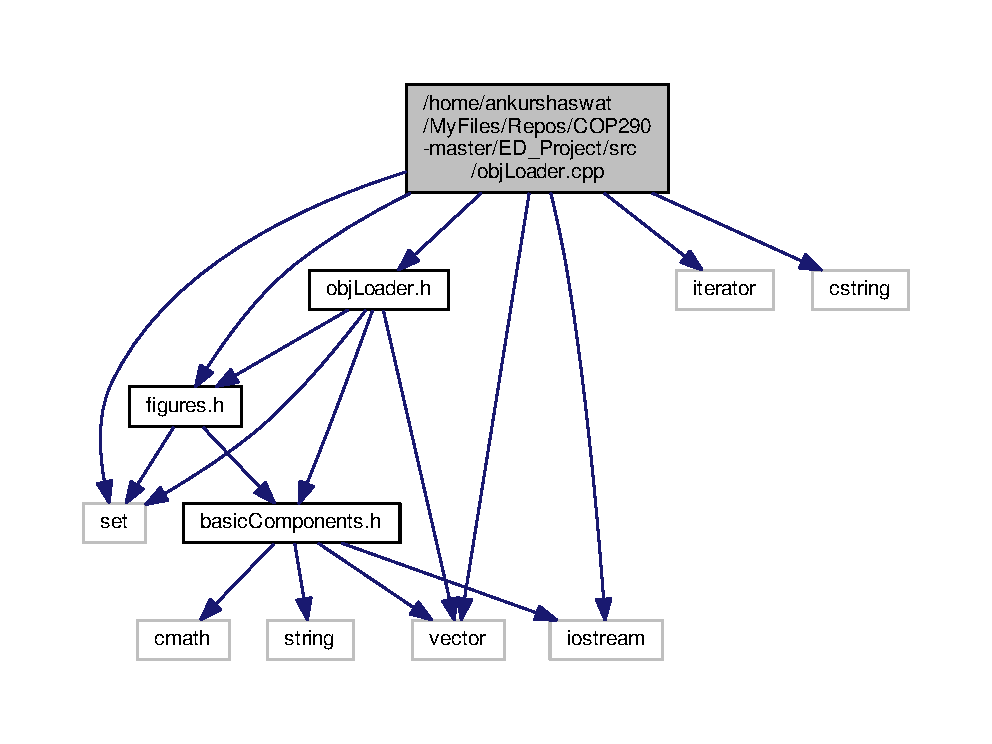
\includegraphics[width=350pt]{objLoader_8cpp__incl}
\end{center}
\end{figure}
\subsection*{Functions}
\begin{DoxyCompactItemize}
\item 
\hyperlink{classFig3D}{Fig3D} \hyperlink{objLoader_8cpp_aceb7a3048c7f82ebf68f0256aedbe70f}{load\+O\+BJ} (const char $\ast$path)
\begin{DoxyCompactList}\small\item\em Function to load O\+BJ file and save its contents into a 3d figure object. \end{DoxyCompactList}\item 
bool \hyperlink{objLoader_8cpp_a1d2e4768c65bd1c911d9810c0d72e227}{get\+\_\+edges3D} (std\+::vector$<$ \hyperlink{structVertice}{Vertice} $>$ \&vertices3D, std\+::vector$<$ std\+::vector$<$ unsigned int $>$ $>$ \&faces\+\_\+vertices, std\+::set$<$ \hyperlink{structEdge}{Edge} $>$ \&edge\+Set)
\end{DoxyCompactItemize}


\subsection{Function Documentation}
\mbox{\Hypertarget{objLoader_8cpp_a1d2e4768c65bd1c911d9810c0d72e227}\label{objLoader_8cpp_a1d2e4768c65bd1c911d9810c0d72e227}} 
\index{obj\+Loader.\+cpp@{obj\+Loader.\+cpp}!get\+\_\+edges3D@{get\+\_\+edges3D}}
\index{get\+\_\+edges3D@{get\+\_\+edges3D}!obj\+Loader.\+cpp@{obj\+Loader.\+cpp}}
\subsubsection{\texorpdfstring{get\+\_\+edges3\+D()}{get\_edges3D()}}
{\footnotesize\ttfamily bool get\+\_\+edges3D (\begin{DoxyParamCaption}\item[{std\+::vector$<$ \hyperlink{structVertice}{Vertice} $>$ \&}]{vertices3D,  }\item[{std\+::vector$<$ std\+::vector$<$ unsigned int $>$ $>$ \&}]{faces\+\_\+vertices,  }\item[{std\+::set$<$ \hyperlink{structEdge}{Edge} $>$ \&}]{edge\+Set }\end{DoxyParamCaption})}

\mbox{\Hypertarget{objLoader_8cpp_aceb7a3048c7f82ebf68f0256aedbe70f}\label{objLoader_8cpp_aceb7a3048c7f82ebf68f0256aedbe70f}} 
\index{obj\+Loader.\+cpp@{obj\+Loader.\+cpp}!load\+O\+BJ@{load\+O\+BJ}}
\index{load\+O\+BJ@{load\+O\+BJ}!obj\+Loader.\+cpp@{obj\+Loader.\+cpp}}
\subsubsection{\texorpdfstring{load\+O\+B\+J()}{loadOBJ()}}
{\footnotesize\ttfamily \hyperlink{classFig3D}{Fig3D} load\+O\+BJ (\begin{DoxyParamCaption}\item[{const char $\ast$}]{path }\end{DoxyParamCaption})}



Function to load O\+BJ file and save its contents into a 3d figure object. 


\hypertarget{program_8cpp}{}\section{/home/ankurshaswat/\+My\+Files/\+Repos/\+C\+O\+P290/\+Project1/\+Code/src/program.cpp File Reference}
\label{program_8cpp}\index{/home/ankurshaswat/\+My\+Files/\+Repos/\+C\+O\+P290/\+Project1/\+Code/src/program.\+cpp@{/home/ankurshaswat/\+My\+Files/\+Repos/\+C\+O\+P290/\+Project1/\+Code/src/program.\+cpp}}


Main file documentation.  


{\ttfamily \#include $<$iostream$>$}\newline
Include dependency graph for program.\+cpp\+:\nopagebreak
\begin{figure}[H]
\begin{center}
\leavevmode
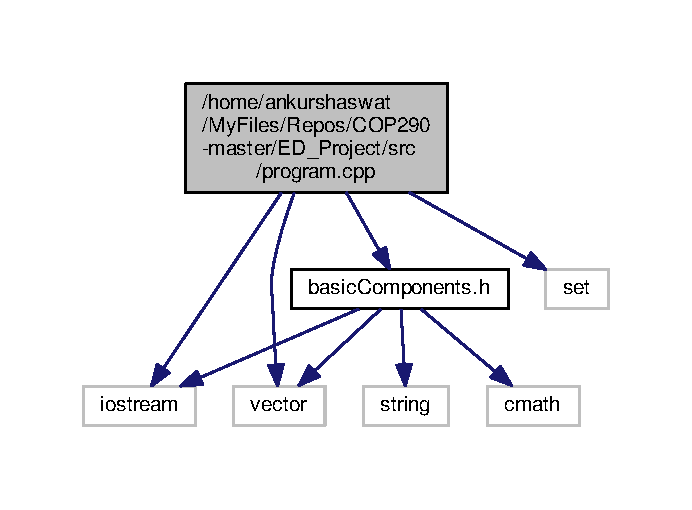
\includegraphics[width=235pt]{program_8cpp__incl}
\end{center}
\end{figure}
\subsection*{Functions}
\begin{DoxyCompactItemize}
\item 
int \hyperlink{program_8cpp_ae66f6b31b5ad750f1fe042a706a4e3d4}{main} ()
\end{DoxyCompactItemize}


\subsection{Detailed Description}
Main file documentation. 

\begin{DoxyAuthor}{Author}
Lastname\+:\+Firstname\+:\+A00123456\+:cscxxxxx 
\end{DoxyAuthor}
\begin{DoxyVersion}{Version}
Revision 1.\+0
\end{DoxyVersion}
Main File \begin{DoxyDate}{Date}
Monday, March 5, 2018 
\end{DoxyDate}


\subsection{Function Documentation}
\mbox{\Hypertarget{program_8cpp_ae66f6b31b5ad750f1fe042a706a4e3d4}\label{program_8cpp_ae66f6b31b5ad750f1fe042a706a4e3d4}} 
\index{program.\+cpp@{program.\+cpp}!main@{main}}
\index{main@{main}!program.\+cpp@{program.\+cpp}}
\subsubsection{\texorpdfstring{main()}{main()}}
{\footnotesize\ttfamily int main (\begin{DoxyParamCaption}{ }\end{DoxyParamCaption})}


\hypertarget{reconstMethods_8cpp}{}\section{/home/ankurshaswat/\+My\+Files/\+Repos/\+C\+O\+P290/working\+\_\+3d\+\_\+to\+\_\+2d/src/reconst\+Methods.cpp File Reference}
\label{reconstMethods_8cpp}\index{/home/ankurshaswat/\+My\+Files/\+Repos/\+C\+O\+P290/working\+\_\+3d\+\_\+to\+\_\+2d/src/reconst\+Methods.\+cpp@{/home/ankurshaswat/\+My\+Files/\+Repos/\+C\+O\+P290/working\+\_\+3d\+\_\+to\+\_\+2d/src/reconst\+Methods.\+cpp}}
{\ttfamily \#include \char`\"{}basic\+Components.\+h\char`\"{}}\newline
{\ttfamily \#include \char`\"{}complex\+Components.\+h\char`\"{}}\newline
{\ttfamily \#include \char`\"{}figures.\+h\char`\"{}}\newline
{\ttfamily \#include \char`\"{}structs.\+h\char`\"{}}\newline
{\ttfamily \#include \char`\"{}reconst\+Methods.\+h\char`\"{}}\newline
{\ttfamily \#include \char`\"{}helperfunctions.\+h\char`\"{}}\newline
{\ttfamily \#include $<$map$>$}\newline
{\ttfamily \#include $<$iostream$>$}\newline
{\ttfamily \#include $<$algorithm$>$}\newline
Include dependency graph for reconst\+Methods.\+cpp\+:
\nopagebreak
\begin{figure}[H]
\begin{center}
\leavevmode
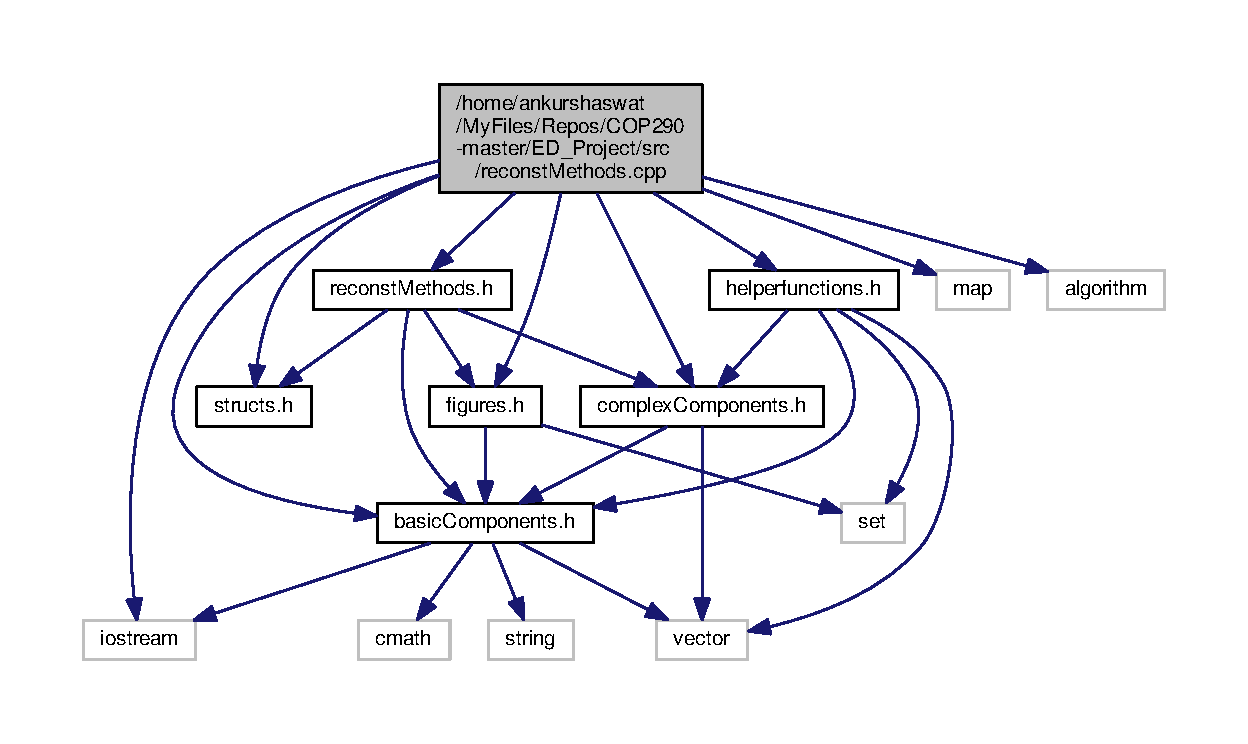
\includegraphics[width=350pt]{reconstMethods_8cpp__incl}
\end{center}
\end{figure}
\subsection*{Functions}
\begin{DoxyCompactItemize}
\item 
std\+::vector$<$ std\+::vector$<$ \hyperlink{structEdge}{Edge} $>$ $>$ \hyperlink{reconstMethods_8cpp_a5b106c1c411ab1e9cbb880661e8702fc}{read\+File} (const char $\ast$path)
\begin{DoxyCompactList}\small\item\em Function to read txt file contatining labelled data of xy , yz and xz views and returns the result as a vector of vector of edges. \end{DoxyCompactList}\item 
\hyperlink{classWireFrame}{Wire\+Frame} \hyperlink{reconstMethods_8cpp_a110e71b7da4f490cc73c09b654d2db99}{const\+Uniq3d\+Edges} (vector$<$ vector$<$ \hyperlink{structEdge}{Edge} $>$ $>$ edge\+Set)
\begin{DoxyCompactList}\small\item\em Function to construct 3d edges from 2d edges by checking the possibility of the edges being projections of each other. \end{DoxyCompactList}\item 
vector$<$ vector$<$ int $>$ $>$ \hyperlink{reconstMethods_8cpp_ad748b0dac80de637f972c4676f8ccdaa}{coplanar\+Edges} (vector$<$ \hyperlink{structEdge}{Edge} $>$ \&edges)
\item 
vector$<$ vector$<$ int $>$ $>$ \hyperlink{reconstMethods_8cpp_aed7e2db16ce5e7210f9f80b20a8af52f}{get\+Edge\+Loops} (vector$<$ \hyperlink{structEdge}{Edge} $>$ \&edges, vector$<$ int $>$ coplanar\+Indices)
\item 
\hyperlink{classFig3D}{Fig3D} \hyperlink{reconstMethods_8cpp_a323870048d29be8ede27a7020e767c79}{wireframe\+To3D} (\hyperlink{classWireFrame}{Wire\+Frame} a)
\begin{DoxyCompactList}\small\item\em Takes a wireframe object and converts it into a 3d object by creating faces by forming edge loops. \end{DoxyCompactList}\end{DoxyCompactItemize}


\subsection{Function Documentation}
\mbox{\Hypertarget{reconstMethods_8cpp_a110e71b7da4f490cc73c09b654d2db99}\label{reconstMethods_8cpp_a110e71b7da4f490cc73c09b654d2db99}} 
\index{reconst\+Methods.\+cpp@{reconst\+Methods.\+cpp}!const\+Uniq3d\+Edges@{const\+Uniq3d\+Edges}}
\index{const\+Uniq3d\+Edges@{const\+Uniq3d\+Edges}!reconst\+Methods.\+cpp@{reconst\+Methods.\+cpp}}
\subsubsection{\texorpdfstring{const\+Uniq3d\+Edges()}{constUniq3dEdges()}}
{\footnotesize\ttfamily \hyperlink{classWireFrame}{Wire\+Frame} const\+Uniq3d\+Edges (\begin{DoxyParamCaption}\item[{vector$<$ vector$<$ \hyperlink{structEdge}{Edge} $>$ $>$}]{edge\+Set }\end{DoxyParamCaption})}



Function to construct 3d edges from 2d edges by checking the possibility of the edges being projections of each other. 

Defines methods required for 3D reconstruction process \mbox{\Hypertarget{reconstMethods_8cpp_ad748b0dac80de637f972c4676f8ccdaa}\label{reconstMethods_8cpp_ad748b0dac80de637f972c4676f8ccdaa}} 
\index{reconst\+Methods.\+cpp@{reconst\+Methods.\+cpp}!coplanar\+Edges@{coplanar\+Edges}}
\index{coplanar\+Edges@{coplanar\+Edges}!reconst\+Methods.\+cpp@{reconst\+Methods.\+cpp}}
\subsubsection{\texorpdfstring{coplanar\+Edges()}{coplanarEdges()}}
{\footnotesize\ttfamily vector$<$ vector$<$int$>$ $>$ coplanar\+Edges (\begin{DoxyParamCaption}\item[{vector$<$ \hyperlink{structEdge}{Edge} $>$ \&}]{edges }\end{DoxyParamCaption})}

Returns coplanar sets of edges of size$>$=3 (each coplanar set is represented as a list of edge indices) \mbox{\Hypertarget{reconstMethods_8cpp_aed7e2db16ce5e7210f9f80b20a8af52f}\label{reconstMethods_8cpp_aed7e2db16ce5e7210f9f80b20a8af52f}} 
\index{reconst\+Methods.\+cpp@{reconst\+Methods.\+cpp}!get\+Edge\+Loops@{get\+Edge\+Loops}}
\index{get\+Edge\+Loops@{get\+Edge\+Loops}!reconst\+Methods.\+cpp@{reconst\+Methods.\+cpp}}
\subsubsection{\texorpdfstring{get\+Edge\+Loops()}{getEdgeLoops()}}
{\footnotesize\ttfamily vector$<$ vector$<$int$>$ $>$ get\+Edge\+Loops (\begin{DoxyParamCaption}\item[{vector$<$ \hyperlink{structEdge}{Edge} $>$ \&}]{edges,  }\item[{vector$<$ int $>$}]{coplanar\+Indices }\end{DoxyParamCaption})}

takes input a set of coplanar edges (as edges + indices) and returns a list of edge loops(candidate faces) formed using these edges (each edge\+Loop is represented by a list of indices) \mbox{\Hypertarget{reconstMethods_8cpp_a5b106c1c411ab1e9cbb880661e8702fc}\label{reconstMethods_8cpp_a5b106c1c411ab1e9cbb880661e8702fc}} 
\index{reconst\+Methods.\+cpp@{reconst\+Methods.\+cpp}!read\+File@{read\+File}}
\index{read\+File@{read\+File}!reconst\+Methods.\+cpp@{reconst\+Methods.\+cpp}}
\subsubsection{\texorpdfstring{read\+File()}{readFile()}}
{\footnotesize\ttfamily std\+::vector$<$std\+::vector$<$\hyperlink{structEdge}{Edge}$>$ $>$ read\+File (\begin{DoxyParamCaption}\item[{const char $\ast$}]{path }\end{DoxyParamCaption})}



Function to read txt file contatining labelled data of xy , yz and xz views and returns the result as a vector of vector of edges. 

\mbox{\Hypertarget{reconstMethods_8cpp_a323870048d29be8ede27a7020e767c79}\label{reconstMethods_8cpp_a323870048d29be8ede27a7020e767c79}} 
\index{reconst\+Methods.\+cpp@{reconst\+Methods.\+cpp}!wireframe\+To3D@{wireframe\+To3D}}
\index{wireframe\+To3D@{wireframe\+To3D}!reconst\+Methods.\+cpp@{reconst\+Methods.\+cpp}}
\subsubsection{\texorpdfstring{wireframe\+To3\+D()}{wireframeTo3D()}}
{\footnotesize\ttfamily \hyperlink{classFig3D}{Fig3D} wireframe\+To3D (\begin{DoxyParamCaption}\item[{\hyperlink{classWireFrame}{Wire\+Frame}}]{a }\end{DoxyParamCaption})}



Takes a wireframe object and converts it into a 3d object by creating faces by forming edge loops. 


\hypertarget{renderMethods_8cpp}{}\section{/home/ankurshaswat/\+My\+Files/\+Repos/\+C\+O\+P290-\/master/\+E\+D\+\_\+\+Project/src/render\+Methods.cpp File Reference}
\label{renderMethods_8cpp}\index{/home/ankurshaswat/\+My\+Files/\+Repos/\+C\+O\+P290-\/master/\+E\+D\+\_\+\+Project/src/render\+Methods.\+cpp@{/home/ankurshaswat/\+My\+Files/\+Repos/\+C\+O\+P290-\/master/\+E\+D\+\_\+\+Project/src/render\+Methods.\+cpp}}
{\ttfamily \#include \char`\"{}basic\+Components.\+h\char`\"{}}\newline
{\ttfamily \#include \char`\"{}obj\+Loader.\+h\char`\"{}}\newline
{\ttfamily \#include \char`\"{}figures.\+h\char`\"{}}\newline
{\ttfamily \#include $<$Qt\+Ui\+Tools$>$}\newline
{\ttfamily \#include $<$iostream$>$}\newline
{\ttfamily \#include $<$vector$>$}\newline
{\ttfamily \#include $<$set$>$}\newline
{\ttfamily \#include $<$cmath$>$}\newline
Include dependency graph for render\+Methods.\+cpp\+:
\nopagebreak
\begin{figure}[H]
\begin{center}
\leavevmode
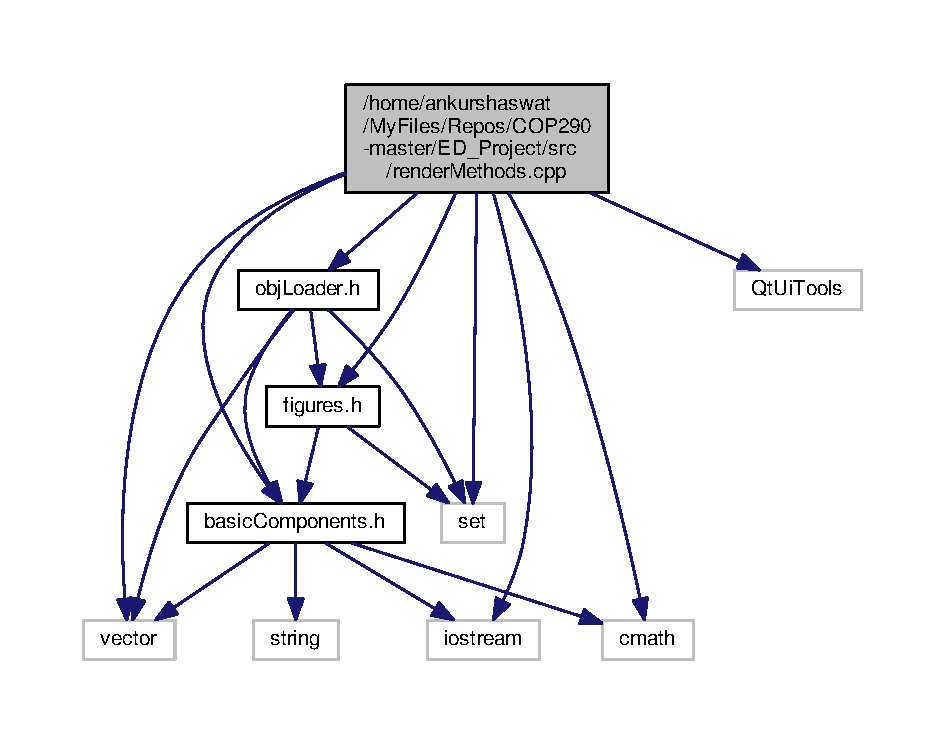
\includegraphics[width=350pt]{renderMethods_8cpp__incl}
\end{center}
\end{figure}
\subsection*{Functions}
\begin{DoxyCompactItemize}
\item 
void \hyperlink{renderMethods_8cpp_a140a5ac6c0e620e7c489498d171be70d}{render2D} (\hyperlink{classFig3D}{Fig3D} \&object3D, Q\+Painter \&painter, int plane, double scale\+\_\+factor)
\item 
void \hyperlink{renderMethods_8cpp_a75faaca4675cd8cd28ae49e79c140c42}{render\+Axes} (\hyperlink{classFig3D}{Fig3D} \&object3D, Q\+Painter \&painter, int plane, double scale\+\_\+factor)
\begin{DoxyCompactList}\small\item\em Function to display axes on the labels for reference. \end{DoxyCompactList}\end{DoxyCompactItemize}


\subsection{Function Documentation}
\mbox{\Hypertarget{renderMethods_8cpp_a140a5ac6c0e620e7c489498d171be70d}\label{renderMethods_8cpp_a140a5ac6c0e620e7c489498d171be70d}} 
\index{render\+Methods.\+cpp@{render\+Methods.\+cpp}!render2D@{render2D}}
\index{render2D@{render2D}!render\+Methods.\+cpp@{render\+Methods.\+cpp}}
\subsubsection{\texorpdfstring{render2\+D()}{render2D()}}
{\footnotesize\ttfamily void render2D (\begin{DoxyParamCaption}\item[{\hyperlink{classFig3D}{Fig3D} \&}]{object3D,  }\item[{Q\+Painter \&}]{painter,  }\item[{int}]{plane,  }\item[{double}]{scale\+\_\+factor }\end{DoxyParamCaption})}

Takes input 3D object , Q\+Painter object, othographic plane (XY /\+Y\+Z/ X\+Z/isometric) and draws the corresponding 2D view on the Q\+Painter object \mbox{\Hypertarget{renderMethods_8cpp_a75faaca4675cd8cd28ae49e79c140c42}\label{renderMethods_8cpp_a75faaca4675cd8cd28ae49e79c140c42}} 
\index{render\+Methods.\+cpp@{render\+Methods.\+cpp}!render\+Axes@{render\+Axes}}
\index{render\+Axes@{render\+Axes}!render\+Methods.\+cpp@{render\+Methods.\+cpp}}
\subsubsection{\texorpdfstring{render\+Axes()}{renderAxes()}}
{\footnotesize\ttfamily void render\+Axes (\begin{DoxyParamCaption}\item[{\hyperlink{classFig3D}{Fig3D} \&}]{object3D,  }\item[{Q\+Painter \&}]{painter,  }\item[{int}]{plane,  }\item[{double}]{scale\+\_\+factor }\end{DoxyParamCaption})}



Function to display axes on the labels for reference. 


%--- End generated contents ---

% Index
\backmatter
\newpage
\phantomsection
\clearemptydoublepage
\addcontentsline{toc}{chapter}{Index}
\printindex

\end{document}
